\documentclass[11pt,a4paper]{article}

% ---------- Packages ----------
\usepackage[margin=1in]{geometry}
\usepackage{amsmath,amssymb}
\usepackage{graphicx}
\usepackage{booktabs}
\usepackage{longtable}
\usepackage{array}
\usepackage{enumitem}
\usepackage[colorlinks=true,linkcolor=blue,citecolor=blue,urlcolor=blue]{hyperref}
\usepackage{titlesec}
\usepackage{xcolor}
\usepackage{tcolorbox}
\tcbuselibrary{skins,breakable}
\usepackage{fancyhdr}
\usepackage{parskip}
\usepackage{tabularx}
\usepackage{tikz}
\usepackage{pgfplots}
\pgfplotsset{compat=1.17}
\usetikzlibrary{arrows.meta,positioning,calc,decorations.markings}

% ---------- Figure box (caption + centering wrapper for tikz/pgfplots figures) ----------
\newtcolorbox{figbox}[1][]{colback=white,colframe=gray!60!black,fonttitle=\bfseries,title=Figure,#1,breakable,center title}

% ---------- Colored boxes for structure ----------
\newtcolorbox{keybox}[1][]{colback=blue!5!white,colframe=blue!40!black,fonttitle=\bfseries,title=Key Idea,#1,breakable}
\newtcolorbox{papbox}[1][]{colback=green!5!white,colframe=green!30!black,fonttitle=\bfseries,title=Paper Summary,#1,breakable}
\newtcolorbox{exambox}[1][]{colback=yellow!10!white,colframe=orange!60!black,fonttitle=\bfseries,title=Likely Exam Point,#1,breakable}

\titleformat{\section}{\normalfont\Large\bfseries\color{blue!40!black}}{\thesection}{1em}{}
\titleformat{\subsection}{\normalfont\large\bfseries}{\thesubsection}{1em}{}

\pagestyle{fancy}
\fancyhf{}
\fancyhead[L]{BI2113 -- Eco-Evo Consolidated Notes}
\fancyhead[R]{\thepage}
\renewcommand{\headrulewidth}{0.4pt}

\title{\textbf{BI2113: Ecology \& Evolution \\ \large Consolidated Course Notes -- Slides + Mandatory/Paper Material}}
\author{Compiled study notes}
\date{Last updated: \today}

\begin{document}
\maketitle

\section*{How to use this document}
This document consolidates all seven topic modules of the course into one self-contained reading. For each topic it covers: (1) the core concepts as presented on the lecture slides (these are, per the instructor's own classification, always examinable), and (2) concise summaries of the procedure/method and conclusions of every research-paper-type reference that the slides cite or attach, since these carry real explanatory weight even when not formally ``on the syllabus.'' Pure textbook chapters attached purely as background (e.g. whole chapters of Molles' or Rockwood's ecology textbooks) are deliberately \emph{not} reproduced in depth -- they exist to elaborate, not to test -- but wherever a concept from a slide needs a textbook-level definition to make sense, that definition is given briefly at 12th-grade-plus baseline. Comparison tables and diagrams are used wherever they make a relationship easier to hold in your head.

\tableofcontents
\newpage

% =====================================================================
\section{Introduction to Biology: Philosophy, Framework, and the Wildebeest Case Study}
% =====================================================================

\subsection{Why does Biology feel so different from Physics?}
The module opens with three ``burning questions'' that most students have at some point: why is biology so memorization-heavy, why is it so description-heavy, and why does it lack a small set of elegant equations from which everything else follows (unlike, say, classical mechanics)? The answer offered is essentially a matter of \textbf{philosophy of biology}: ecology and evolutionary biology sit in a middle ground between fully a-historical, law-governed sciences like physics and fully historical, idiosyncratic disciplines like paleontology. Because living systems carry history (contingent past events shape their present state) and are built from enormously many interacting parts, they resist the kind of universal, exceptionless laws that physics enjoys. This is why the field leans on \textbf{description} and \textbf{statistical, conditional relationships} rather than deterministic equations.

\begin{keybox}
Biology (esp. ecology/evolution) occupies a middle ground: not as law-like as physics, not as purely narrative as paleontology. Its subject matter is historical, contingent, and multi-scale, so mathematical formalization is harder and results are usually statistical/conditional rather than universal.
\end{keybox}

\subsection{The Framework of Biology: levels of organization}
Biological systems are organized into a hierarchy of scales, and the course (BI2113) situates itself within this hierarchy. Two versions of the hierarchy are useful to keep in mind, one running over very long (evolutionary) timescales and one over shorter (ecological) timescales.

\begin{center}
\begin{tabularx}{\textwidth}{@{}l X X@{}}
\toprule
\textbf{Level} & \textbf{Longer/Evolutionary-timescale view} & \textbf{Shorter/Ecological-timescale view} \\
\midrule
Biosphere & \multicolumn{2}{c}{Sum of all ecosystems on Earth} \\
Biome & \multicolumn{2}{c}{Large-scale regions defined by climate/vegetation} \\
Ecosystem & \multicolumn{2}{c}{Community + abiotic environment (``changing'')} \\
Community & \multicolumn{2}{c}{All populations of different species co-occurring} \\
Population & Changed trait values $\to$ \emph{microevolution} & Population-level dynamics (birth/death/growth) \\
Individual & Re-arrangement of genes, reduction division $\to$ \emph{speciation} & Single organism's physiology/behaviour \\
Organ system / Organ / Tissue / Cell & Gamete, fertilization $\to$ \emph{macroevolution} & Sub-organismal structure \\
Biomolecules & \multicolumn{2}{c}{DNA, proteins, etc.} \\
\bottomrule
\end{tabularx}
\end{center}

\textbf{BI2113 sits at the Population $\to$ Community $\to$ Ecosystem band}, i.e., it is primarily about ecology (population dynamics, species interactions) with a bridge into microevolution (changed trait values in a population).

\subsection{Peculiarities/features of biological systems to keep watching for}
\begin{itemize}[leftmargin=1.5em]
\item \textbf{Diversity and interconnectedness} -- both within one level (e.g., many species in a community) and across levels (e.g., a gene change affecting community structure).
\item \textbf{Stochasticity} -- biological systems are inherently ``chancy''; outcomes are probabilistic, not deterministic.
\item \textbf{Historicity} -- present states depend on the particular historical path taken, not just current conditions.
\item \textbf{Emergence} -- reductionism (explaining the whole purely from its parts) often fails; higher-level patterns can't always be predicted just by looking at lower-level components.
\end{itemize}

\begin{exambox}
If asked ``why is biology hard to formalize mathematically,'' the expected answer structure is: (i) historicity/contingency, (ii) stochasticity, (iii) emergence defeating simple reductionism, (iv) resulting reliance on statistical/conditional relationships instead of universal laws.
\end{exambox}

\subsection{The course's approach given this trade-off}
Because of the fundamental \textbf{breadth vs.\ depth trade-off}, BI2113 explicitly chooses \textbf{breadth}. Its four-pronged approach:
\begin{enumerate}[leftmargin=1.5em]
\item Oversimplified mathematical modelling (simple models with caveats, not fully realistic ones).
\item Focus on concepts over exhaustive detail.
\item Historical narrative (how ideas/knowledge developed).
\item Examining the pedagogy itself (thinking about how the subject is taught/learned).
\end{enumerate}

\subsection{Reading-material classification used throughout the course}
This classification recurs in every module, so it is worth internalizing once:
\begin{center}
\begin{tabularx}{\textwidth}{@{}l X X@{}}
\toprule
\textbf{Category} & \textbf{What it is} & \textbf{Exam relevance} \\
\midrule
Mandatory reading & Entry-level book chapters; the lecture slides themselves are automatically in this category & Fully examinable -- this is the syllabus \\
Detailed / Recommended reading & Slightly more detailed book chapters/papers/extracts that elaborate on class topics, same conceptual level but more information & Explicitly \emph{not} examinable \\
Papers & Research papers/monograph chapters on advanced aspects & Not examinable directly, but meant to build a feel for how scientific research is actually conducted \\
\bottomrule
\end{tabularx}
\end{center}

\subsection{Case study: the Serengeti Wildebeest Migration}
The wildebeest (\emph{Connochaetes taurinus}) migration is used as the running example to illustrate ``how'' and ``why'' questions in biology.

\subsubsection*{The ``How'' question: mechanism of the $\sim$1500 km/year migration}
\begin{itemize}[leftmargin=1.5em]
\item \textbf{Muscle efficiency}: wildebeest muscles are exceptionally efficient locomotor engines -- about \textbf{62.6\% efficiency}, compared to \textbf{41.8\% in cows} and \textbf{34\% in mice} (Curtin et al. 2018, \emph{Nature}). This remarkable efficiency is part of what makes such long-distance travel energetically feasible.
\item \textbf{Reproductive adaptations}: (i) calving is highly \emph{synchronous}, which creates a temporary glut of prey that ``swamps'' predators (predator satiation) so that, proportionally, fewer calves are taken; (ii) wildebeest calves are \emph{precocious} -- able to stand and run within minutes of birth, which is essential for a population that must keep moving.
\end{itemize}

\subsubsection*{The ``Why'' question: what benefit does migration confer?}
This requires looking at the Serengeti-Mara landscape itself. Two headline consequences of the migration on the wider ecosystem, both given as concrete examples in the slides:
\begin{enumerate}[leftmargin=1.5em]
\item \textbf{Mass drowning events}: Large numbers of wildebeest drown annually while crossing the Mara River. Rather than being simply a tragic loss, this turns out to be ecologically important: Subalusky et al. (2017, \emph{PNAS}) showed these mass drownings significantly influence nutrient cycling and storage in the river -- essentially, wildebeest carcasses are a substantial, recurring nutrient subsidy to the river ecosystem.
\item \textbf{Fire}: the migration interacts with fire regimes in the ecosystem (grazing pressure alters fuel loads/vegetation structure across the landscape).
\end{enumerate}

\begin{papbox}[title={Paper Summary: Holdo, Holt \& Fryxell (2009), \textit{Am. Nat.} -- ``Opposing Rainfall and Plant Nutritional Gradients Best Explain the Wildebeest Migration in the Serengeti''}]
\textbf{Question:} What proximate factors actually drive wildebeest onto the plains at the start of the wet season, given that rainfall (and hence total forage) is actually \emph{higher} in the woodlands year-round?

\textbf{Procedure:} Built a rainfall-driven simulation model of grass dynamics + wildebeest movement. Tested 14 candidate models of adaptive movement (differing in what cue movement responds to: grass biomass, green-grass intake rate, plant nitrogen/protein content, tree-cover suppression of grass, etc.) against 3 years of observed monthly wildebeest distribution data, using information-theoretic model comparison at two spatial scales (5 km and 25 km resolution).

\textbf{Key conclusions:}
\begin{itemize}[leftmargin=1.3em,nosep]
\item The best-fitting model was the one combining \emph{green grass intake rate} + \emph{plant nitrogen (protein) concentration} + \emph{tree-cover suppression of grass} -- i.e., digestive constraints and protein requirements, not simply ``more grass,'' drive the migration.
\item Crucially, the plains (rainfall-poor) have volcanic, nutrient-rich soils, while the woodlands (rainfall-rich) sit on sandier, less fertile soils. This creates an \textbf{opposing gradient}: rainfall increases from southeast to northwest, while soil/plant nitrogen decreases in the same direction. Wildebeest exploit the high-protein plains specifically when the rains make them accessible.
\item Migration only emerges in the model when wildebeest can track resources over large spatial scales ($\sim$180--100 km neighborhood); purely local resource-tracking fails to reproduce migration.
\item This model outperformed a prior evolutionary-programming model (Boone et al. 2006) that used a rainfall/NDVI ratio, fitting observed distributions substantially better (27.4\% vs.\ 13.4\% agreement at 5 km resolution).
\end{itemize}
\textit{Instructor's note: don't get bogged down in the model mechanics -- the intro and discussion carry the exam-relevant takeaway, which is the opposing-gradients idea.}
\end{papbox}

\begin{papbox}[title={Paper Summary: Hopcraft et al. (2015), in \textit{Serengeti IV} -- ``Why Are Wildebeest the Most Abundant Herbivore in the Serengeti Ecosystem?''}]
\textbf{Question:} Wildebeest outnumber every other herbivore combined in the Serengeti (6$\times$ more numerous than the next-most-abundant species, zebra). Why?

\textbf{Procedure/Approach:} A structured, three-part comparative argument (not a single experiment) that successively compares wildebeest against (a) their closest relatives (topi, hartebeest), (b) their own resident vs.\ migratory subpopulations, and (c) another migratory species (zebra).

\textbf{Key conclusions (built up step by step):}
\begin{enumerate}[leftmargin=1.3em,nosep]
\item \emph{Biology alone is insufficient.} Wildebeest have a flat, wide dental arcade suited to rapidly cropping short, mat-forming, nutritious grasses (unlike topi/hartebeest, adapted to picking leaves off taller, structurally complex grasses), and highly synchronous, predator-swamping calving. These traits give some advantage but cannot alone explain the scale of dominance (similar advantages exist in some other species without similar abundance).
\item \emph{Resident wildebeest are far less abundant than migrants} -- residents are restricted to the few patches where fine-scale grass heterogeneity and $>$900 mm annual rainfall with permanent water co-occur; this shows suitable habitat + predation constrain non-migrants.
\item \emph{Migration alone is not sufficient either} -- zebra also migrate in the Serengeti, yet remain $\sim$6$\times$ less abundant than wildebeest. The likely reason is that zebra populations are regulated more by predation (top-down), while wildebeest, thanks to superior digestive efficiency on high-quality grass, are comparatively less food/predation limited.
\item \emph{Overall answer}: superabundance is the product of a tight match between (i) wildebeest's specific digestive/reproductive biology, (ii) their migratory capacity, and (iii) the Serengeti's unique countergradient of rainfall and soil fertility that produces a huge (3,500+ km$^2$), spatially accessible zone of high-quality grass. General lesson: migratory superabundance requires refuge areas, ephemeral-but-high-quality resources, and connectivity between patches -- when these three line up for a species (as they do for wildebeest here), that species can dominate.
\end{enumerate}
\end{papbox}

\begin{exambox}
Likely conceptual question format: ``Explain why the wildebeest is the dominant herbivore in the Serengeti using both a biological and an environmental argument.'' Answer should combine: digestive/reproductive traits (Hopcraft et al.) $+$ the opposing rainfall/nutrient gradient enabling long-range resource tracking (Holdo et al.) $+$ the general recipe (refuge + ephemeral high-quality resource + connectivity).
\end{exambox}

\subsection{Course logistics/tips (from the slides)}
\begin{itemize}[leftmargin=1.5em]
\item Memorize the experimental/case-study examples (e.g., wildebeest numbers above) -- these anchor exam answers.
\item Think critically and challenge claims wherever possible.
\item Reading beyond the minimum is encouraged (though only the ``mandatory'' tier is strictly examinable).
\item Solve numerical problems only \emph{after} the underlying concept is understood, not by rote formula plugging.
\end{itemize}

\newpage

% =====================================================================
\section{Structured Population Models: From Cohort Life Tables to Age/Stage-Structured Dynamics}
% =====================================================================

\subsection{Setting the stage: what is population ecology?}
Population ecology is introduced as a subset of the broader question ``why study populations at all?'' Human demography (the study of human populations) is presented as a special case of the general field of \textbf{population ecology}. A \textbf{population} is defined simply as \emph{a group of similar individuals, inhabiting a defined space at a given time}.

\begin{keybox}
Reasons to study (non-human) populations: conservation of endangered species; management of economically important species (agriculture, fisheries); management of harmful species (pests, invasives); populations are the fundamental unit of evolution. What population ecologists actually study, in three buckets: \textbf{Distribution} (spatial pattern), \textbf{Demography} (age structure, survivorship, birth rate), \textbf{Dynamics} (how numbers change in time and space). \textbf{Population dynamics} = the study of how and why population numbers change in time and space.
\end{keybox}

\subsection{Cohort life tables and survivorship curves: \textit{Phlox drummondii}}
The motivating question: if you wanted to document how the numbers in a population change over time, starting from the simplest possible case (a single cohort, no new births added), how would you do it? The slides walk through the classic cohort life-table analysis of the annual plant \emph{Phlox drummondii} (data: Leverich \& Levin, 1979), starting from 996 individuals.

\begin{center}
\begin{tabular}{@{}ccccc@{}}
\toprule
Class $x$ & Age (days) & $l_x$ (survival proportion) & $m_x$ (avg.\ seeds/indiv.) & $l_x m_x$ \\
\midrule
1 & 0--299 & 1.0000 & 0.0000 & 0.0000 \\
2 & 299--306 & 0.1586 & 0.3352 & 0.0532 \\
3 & 306--313 & 0.1546 & 0.7963 & 0.1231 \\
4 & 313--320 & 0.1516 & 2.3995 & 0.3638 \\
5 & 320--327 & 0.1476 & 3.1094 & 0.4589 \\
6 & 327--334 & 0.1365 & 2.5411 & 0.3469 \\
7 & 334--341 & 0.1054 & 3.1589 & 0.3330 \\
8 & 341--348 & 0.0743 & 8.6625 & 0.6436 \\
9 & 348--355 & 0.0221 & 4.3072 & 0.0952 \\
10 & 355--362 & 0.0000 & 0.0000 & 0.0000 \\
\bottomrule
\end{tabular}
\end{center}

\begin{keybox}
$R_0$ = \textbf{net per-capita reproductive rate} = the average number of offspring left per individual over its lifetime = $\sum_x l_x m_x$ (sum of the last column above). This single number summarizes whether a cohort is, on average, replacing itself.
\end{keybox}

From data like this, \textbf{survivorship curves} (log(number surviving) vs.\ age) are drawn, and three idealized types are distinguished:
\begin{itemize}[leftmargin=1.5em]
\item \textbf{Type I}: mortality rates are low until late in life (survivorship stays high, then drops sharply near the end of the lifespan) -- typical of species with strong parental care/few offspring, e.g.\ large mammals, humans in developed settings.
\item \textbf{Type II}: a constant \emph{proportion} of individuals die throughout the life cycle (straight diagonal line on the log-survivorship plot) -- e.g.\ many birds, some reptiles.
\item \textbf{Type III}: juvenile mortality is very high; individuals that survive past that initial bottleneck have comparatively high survivorship afterwards -- typical of species with many offspring and little parental care, e.g.\ most plants (including \textit{Phlox}), fish, marine invertebrates.
\end{itemize}

\begin{exambox}
\textbf{Why is the survivorship-curve $y$-axis plotted on a log scale, not linear?} Because what matters biologically is the \emph{per-capita} (proportional) mortality rate, not the raw number of deaths. On a linear scale, a constant proportional death rate (Type II) looks like it accelerates over time (more individuals die in absolute terms early on, simply because there were more individuals alive then), which is visually misleading. On a log scale, a constant proportional mortality rate shows up as a straight line, letting you correctly compare mortality \emph{rates} across different time periods or different absolute population sizes. (Concretely: if 60\% of individuals die between age 1--2 \emph{and} 60\% die between age 2--3, the per-capita mortality rate is identical in both intervals even though the absolute numbers of deaths differ -- only the log scale makes this visually obvious.) Also remember: these three types are \emph{idealized}; real populations show mixtures/approximations of them, not clean textbook curves.
\end{exambox}

\begin{figbox}[title={The three idealized survivorship curve types}]
\centering
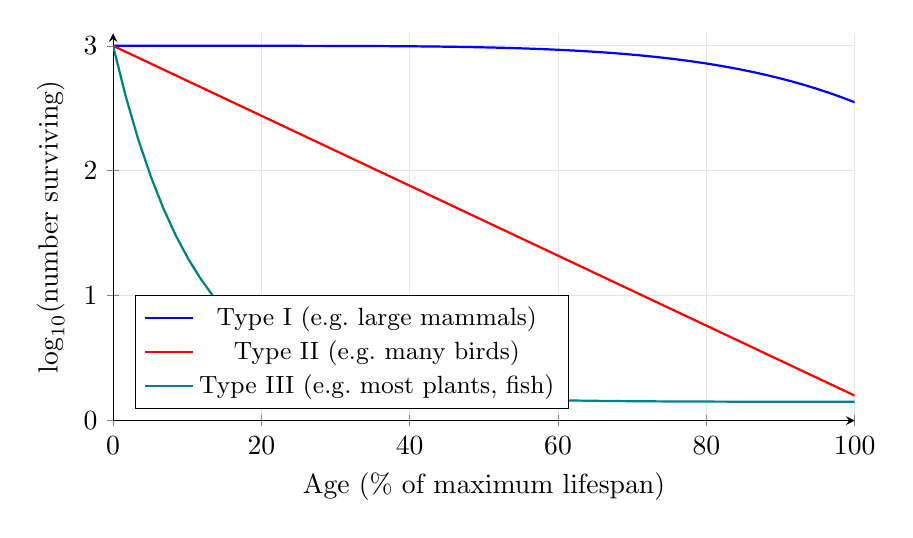
\begin{tikzpicture}
\begin{axis}[
  width=11cm, height=6.5cm,
  xlabel={Age (\% of maximum lifespan)},
  ylabel={$\log_{10}$(number surviving)},
  xmin=0, xmax=100, ymin=0, ymax=3.1,
  xtick={0,20,40,60,80,100},
  ytick={0,1,2,3},
  legend pos=south west,
  legend style={font=\small},
  axis lines=left,
  enlargelimits=false,
  grid=major, grid style={gray!20}
]
% Type I: stays high, drops sharply late
\addplot[thick, blue, domain=0:100, samples=60] {3 - 0.0000018*x^5.2/100000};
\addlegendentry{Type I (e.g.\ large mammals)}
% Type II: straight diagonal line (constant proportional mortality)
\addplot[thick, red, domain=0:100, samples=2] {3 - 0.028*x};
\addlegendentry{Type II (e.g.\ many birds)}
% Type III: crashes early, then flattens
\addplot[thick, teal, domain=0:100, samples=60] {0.15 + 2.85*exp(-0.09*x)};
\addlegendentry{Type III (e.g.\ most plants, fish)}
\end{axis}
\end{tikzpicture}

\vspace{2mm}
\footnotesize\emph{Schematic, not fitted to data.} Type I: mortality concentrated late in life (curve stays flat, then drops). Type II: constant per-capita mortality at every age (straight line on this log-linear plot). Type III: heavy early/juvenile mortality (steep initial drop), then a long flat tail of good survivorship for those that make it past the bottleneck.
\end{figbox}

\subsection{Age-structured dynamics: the Leslie Matrix}
The cohort life-table approach above has a major simplification baked in: no new offspring are added, so you're only ever watching one cohort age and die out. The natural next step (``remove some constraints: let there be kids'') is \textbf{age-structured dynamics}, formalized via the \textbf{Leslie matrix}.

A toy example used in the slides: four age classes, with survival probabilities $P_x$ (probability of surviving from class $x$ to class $x+1$) and fecundities $F_x$ (offspring contributed by class $x$):

\begin{center}
\begin{tabular}{@{}cccc@{}}
\toprule
Age class $x$ & $P_x$ & $F_x$ \\
\midrule
1 & 0.5 & 0 \\
2 & 0.2 & 2 \\
3 & 0.1 & 1 \\
4 & 0 & 1 \\
\bottomrule
\end{tabular}
\end{center}

Starting from 200 individuals all in age class 0 and simulating forward 200 time steps produces several striking, general patterns:
\begin{itemize}[leftmargin=1.5em]
\item After initial oscillations, \textbf{total population size grows monotonically and exponentially}.
\item The \emph{relative proportions} of the different age classes settle down to a constant ratio -- this is the \textbf{stable age distribution (SAD)}: the proportion of the population in each age class, once transients have died out. In the worked example, the SAD converges to roughly 63.5\% class 0, 30.2\% class 1, 5.7\% class 2, 0.5\% class 3.
\item Once the SAD is reached, the ratio $N_{t+1}/N_t$ converges to a single constant, $\lambda$ (here $\lambda \approx 1.05082$), which then fully describes the population's long-run growth rate.
\end{itemize}

\begin{keybox}
\textbf{The mathematical structure behind this (for the mathematically inclined; conceptually optional but useful):} $\lambda$ is the \textbf{dominant eigenvalue} of the Leslie matrix, and the SAD is the corresponding (right) \textbf{eigenvector}. Because a Leslie matrix is non-negative, the \textbf{Perron--Frobenius theorem} guarantees at least one real eigenvalue exists; if there are several, the largest in magnitude is the ``dominant'' one, and its eigenvector gives the SAD. This general behaviour (convergence to exponential growth at rate $\lambda$, with a stable age distribution) holds for \emph{any} biologically realistic Leslie matrix, not just this toy example. (Source for the underlying math: Caswell 1997 -- see Section~\ref{sec:caswell-summary} below.)
\end{keybox}

\begin{exambox}
Conceptual point likely to be tested: \emph{why} does the population eventually grow exponentially at a fixed rate $\lambda$ with a fixed age structure, even though it started at an artificial all-one-age-class initial condition? Answer: any non-negative population vector, repeatedly multiplied by the same projection matrix, converges onto the dominant eigenvector direction (the SAD) regardless of starting condition -- this is a general property of such matrices (Perron--Frobenius), not a coincidence of the particular numbers chosen.
\end{exambox}

\subsection{Applying stage-structured models: conservation of the loggerhead sea turtle}
\label{sec:turtle-case-study}
The Leslie/age-structured framework above assumes you can cleanly assign individuals to \emph{chronological age} classes. For many organisms (including sea turtles), age is hard to measure directly, but \emph{life-history stage} (egg/hatchling, small juvenile, large juvenile, subadult, adult) is much easier to observe and is demographically more meaningful anyway. This motivates \textbf{stage-structured} matrix models, illustrated via the conservation of the loggerhead sea turtle (\emph{Caretta caretta}), originally developed by Crouse et al. (1987) and refined by Crowder et al. (1994).

In a stage-structured matrix, each stage class has two associated probabilities per time step:
\begin{itemize}[leftmargin=1.5em]
\item $P_i$ = probability of \textbf{surviving and remaining} in the same stage class,
\item $G_i$ = probability of \textbf{surviving and growing} into the next stage class.
\end{itemize}
so the projection matrix takes the banded form
\[
A = \begin{pmatrix}
P_1 & F_2 & F_3 & F_4 & F_5 \\
G_1 & P_2 & 0 & 0 & 0 \\
0 & G_2 & P_3 & 0 & 0 \\
0 & 0 & G_3 & P_4 & 0 \\
0 & 0 & 0 & G_4 & P_5
\end{pmatrix},
\]
where fecundity $F_i$ only enters from stages capable of reproducing (adults, and in some formulations, subadults).

\begin{figbox}[title={Life-cycle graph for the five-stage loggerhead turtle model}]
\centering
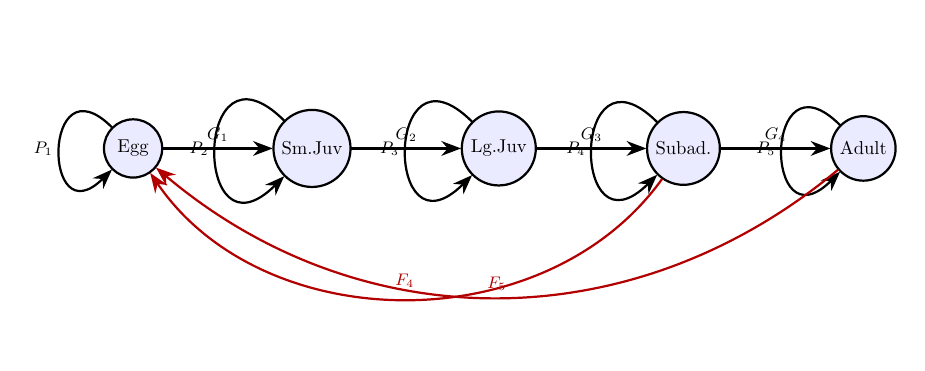
\begin{tikzpicture}[scale=0.82, every node/.style={scale=0.82}, transform shape,
  node distance=1.7cm,
  stage/.style={circle, draw, thick, minimum size=1.1cm, fill=blue!8},
  >={Stealth[length=2.5mm]}
]
\node[stage] (s1) {Egg};
\node[stage, right=of s1] (s2) {Sm.Juv};
\node[stage, right=of s2] (s3) {Lg.Juv};
\node[stage, right=of s3] (s4) {Subad.};
\node[stage, right=of s4] (s5) {Adult};

% growth arrows G_i
\draw[->, thick] (s1) -- (s2) node[midway, above] {\small $G_1$};
\draw[->, thick] (s2) -- (s3) node[midway, above] {\small $G_2$};
\draw[->, thick] (s3) -- (s4) node[midway, above] {\small $G_3$};
\draw[->, thick] (s4) -- (s5) node[midway, above] {\small $G_4$};

% self-loops P_i (stay in stage)
\foreach \n/\lab in {s1/P_1, s2/P_2, s3/P_3, s4/P_4, s5/P_5}{
  \draw[->, thick] (\n) to[out=135,in=225,looseness=6] node[left]{\small $\lab$} (\n);
}

% fecundity arrows F_i back to stage 1 (from subadult and adult)
\draw[->, thick, red!70!black] (s5) to[bend left=40] node[above]{\small $F_5$} (s1);
\draw[->, thick, red!70!black] (s4) to[bend left=55] node[above=2pt]{\small $F_4$} (s1);
\end{tikzpicture}

\vspace{2mm}
\footnotesize Black arrows: survival transitions ($P_i$ = stay in stage, $G_i$ = grow to next stage). Red arrows: fecundity ($F_i$) -- new eggs contributed by reproductive stages, closing the life cycle. This graph is exactly what the projection matrix $A$ on the left encodes numerically: reading down a column of $A$ gives the outgoing arrows from that stage's node.
\end{figbox}

\begin{exambox}
\textbf{Key motivating question, asked directly on the slides:} given the observed pattern of survivorship/mortality across stages, \emph{which} stage should conservation efforts target -- and \emph{how much} improvement is actually needed there (occasional intervention, or all-the-time)? This ``where should we intervene'' framing, backed by a sensitivity/elasticity analysis of the matrix, is the core logical structure of the whole case study and a natural essay-question shape.
\end{exambox}

\begin{papbox}[title={Paper Summary: Crowder, Crouse, Heppell \& Martin (1994), \textit{Ecol.\ Appl.} -- ``Predicting the Impact of Turtle Excluder Devices on Loggerhead Sea Turtle Populations''}]
\textbf{Question:} All five US sea-turtle species are endangered/threatened, and shrimp trawling (with $>$40{,}000 estimated sea-turtle deaths/year) is the single largest human-caused source of mortality. Given limited conservation resources, \emph{which life stage} should interventions target, and what population-level recovery can be expected from turtle excluder devices (TEDs -- escape hatches fitted to trawl nets)?

\textbf{Procedure:} Simplified Crouse et al.'s (1987) seven-stage loggerhead matrix model to a five-stage model (egg/hatchling, small juvenile, large juvenile, subadult, adult), by merging three adult substages that shared the same survivorship. Performed a full \textbf{sensitivity/elasticity analysis} of the projection matrix (elasticity = proportional sensitivity of $\lambda$ to a parameter), separately for survivorship-within-stage, growth-to-next-stage, and stage duration. Then ran forward simulations of the model under different management scenarios: (i) no TEDs (status quo decline), (ii) ``seasonal offshore'' TED regulation (as actually mandated 1990--1992), and (iii) expanded year-round TED regulation.

\textbf{Key conclusions:}
\begin{itemize}[leftmargin=1.3em,nosep]
\item \textbf{Population growth rate ($\lambda$) is far more sensitive to survivorship-within-a-stage than to growth-rate-between-stages or to fecundity.} Among stages, \textbf{large juvenile survival} has by far the largest effect on $\lambda$, followed by small juvenile survival.
\item This matches independent field data: large juveniles are the single most common size class among sea turtles found stranded dead on beaches, and 70--80\% of strandings are attributed to trawl-fishery interactions.
\item \textbf{A 10\% reduction in mortality in any one stage is not enough} -- the population still declines. A \textbf{50\% reduction in large-juvenile mortality} is enough to flip the population from declining to recovering; a 50\% reduction in any \emph{other} stage's mortality only slows the decline. A 90\% mortality reduction in any stage \emph{except} eggs/hatchlings would allow growth.
\item Critically, \textbf{even perfect (100\%) egg/hatchling survival alone cannot make the population grow} -- egg-stage conservation (the traditional focus of turtle conservation: nest protection, hatcheries) is therefore \emph{not} where effort should concentrate, however intuitive it may seem.
\item Simulated recovery under 1990--1992-style ``seasonal offshore'' TED use is slow: $\gtrsim$70 years needed for an order-of-magnitude population increase. Good compliance with \textbf{year-round} TED requirements in all waters could nearly \textbf{double} that rate of increase.
\item A subtlety for beach-survey interpretation: because of shifting age/stage structure as the population responds to TEDs, the \emph{number of nesting females} is predicted to show a transient increase, then a plateau or slight dip around 10--15 years post-regulation, before rising again -- a non-monotonic trajectory that could otherwise be misread as the policy ``not working.''
\item The authors explicitly caution that quantitative projections are uncertain (limited demographic data, several modelling assumptions) and should not be extended uncritically to other sea-turtle species with different life histories.
\end{itemize}
\end{papbox}

\begin{exambox}
Likely conceptual question: ``Why does the loggerhead model recommend protecting large juveniles rather than eggs, even though eggs have the lowest survivorship?'' Expected answer: population growth rate is most \emph{elastic} to survivorship in stages that (a) already contribute many surviving individuals forward and (b) have a long stage duration, so gains compound; the egg stage has enormous natural mortality that is largely compensated for elsewhere in the life cycle, so even eliminating it entirely cannot overcome mortality bottlenecks later in life. This is a general lesson in matrix population models, not specific to turtles: \emph{the numerically ``worst'' stage is not necessarily the most effective stage to intervene on} -- elasticity, not raw mortality, tells you where to act.
\end{exambox}

The applied policy consequence, per the slides: fish trawling (and shrimp trawling especially, with an average bycatch of \textbf{5.7 kg of bycatch per kg of shrimp caught}) was identified as the dominant source of large-juvenile/subadult mortality. Simulations showed that \emph{occasional} TED use would need $\sim$70 years for a substantial population effect, so all-time (not just seasonal) TED use was recommended; India's own government legislated mandatory TED use in shrimp trawling in 1996.

\begin{papbox}[title={Paper Summary: Caswell (1997), \textit{Matrix Methods for Population Analysis} (Ch.\ 2 in Tuljapurkar \& Caswell, \textit{Structured-Population Models in Marine, Terrestrial and Freshwater Systems})}]
\label{sec:caswell-summary}
This is the mathematical-methods reference underlying both the age-structured (Leslie) and stage-structured matrix machinery used throughout this topic; it is a methods chapter rather than an empirical study, so the ``exam-relevant'' takeaway is really just knowing what it establishes, not its own findings. It formalizes how to build a matrix population model in general: choosing \emph{i-state variables} (age, size, stage, location -- whatever determines an individual's response to its environment), discretizing them into stage classes, encoding the life cycle as a \emph{life-cycle graph}, and assembling the projection matrix $\mathbf{A}$ such that $\mathbf{n}(t+1) = \mathbf{A}\,\mathbf{n}(t)$. It develops (via the Perron--Frobenius theorem, already used above) why such matrices generically produce a single dominant growth rate $\lambda$ and an associated stable stage distribution, and introduces \textbf{sensitivity and elasticity analysis} -- the technique Crowder et al.\ (1994) used to identify large-juvenile survival as the key lever -- as a general tool for asking ``how much does $\lambda$ change if I perturb this one matrix entry?''
\end{papbox}

\subsection{A comparison: age-structured vs.\ stage-structured models}
\begin{center}
\begin{tabularx}{\textwidth}{@{}l X X@{}}
\toprule
& \textbf{Age-structured (classic Leslie matrix)} & \textbf{Stage-structured} \\
\midrule
Classes represent & Chronological age (discrete units, e.g.\ years) & Life-history stage (egg, juvenile, adult, \ldots), which may span variable/unknown durations \\
Transition structure & Individuals in class $x$ either die or advance exactly one class per step & Individuals may survive \emph{and stay} in the same stage ($P_i$) or survive \emph{and advance} ($G_i$) -- self-loops allowed \\
Best suited to & Organisms where age is reliably known/measured & Organisms where stage/size is easier to observe than true age, or where demographic rates depend more on stage than age (e.g.\ sea turtles, many plants) \\
Long-run behaviour & Converges to exponential growth at rate $\lambda$ with a stable \emph{age} distribution & Converges to exponential growth at rate $\lambda$ with a stable \emph{stage} distribution -- same underlying Perron--Frobenius logic \\
\bottomrule
\end{tabularx}
\end{center}

\subsection{Coda: back to humans -- age pyramids}
The slides briefly return to human demography: an \textbf{age pyramid} (population count by age band, split by sex) is essentially a snapshot of a population's age structure, and its shape encodes $\lambda$ directly -- the \textbf{greater $\lambda$ is, the broader the base} of the pyramid (many young relative to old, i.e.\ a growing population), while a \textbf{narrow base signals a declining population}. This is the same SAD logic from the Leslie-matrix toy example above, just applied to real human population data instead of a simulation.

\begin{figbox}[title={Age-pyramid shapes and what they say about $\lambda$}]
\centering
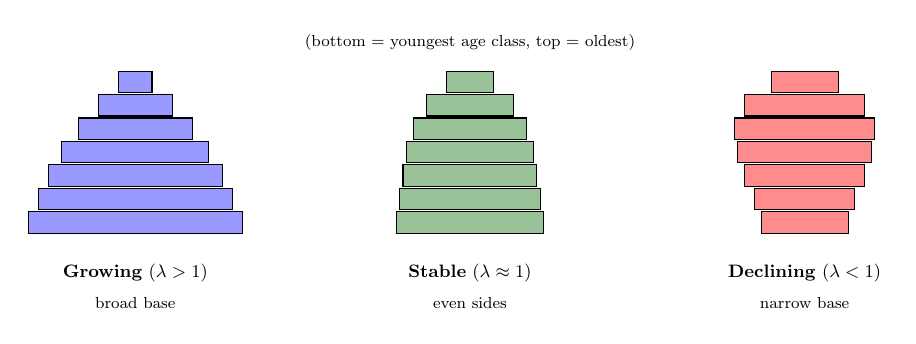
\begin{tikzpicture}[scale=0.85, every node/.style={scale=0.85}, transform shape]
% Growing population (broad base) - lambda > 1
\begin{scope}[xshift=0cm]
\foreach \i/\w in {0/3.2,1/2.9,2/2.6,3/2.2,4/1.7,5/1.1,6/0.5}{
  \draw[fill=blue!40] (-\w/2,\i*0.35) rectangle (\w/2,\i*0.35+0.32);
}
\node at (0,-0.6) {\small \textbf{Growing} ($\lambda>1$)};
\node at (0,-1.05) {\footnotesize broad base};
\end{scope}
% Stable population (rectangle-ish)
\begin{scope}[xshift=5cm]
\foreach \i/\w in {0/2.2,1/2.1,2/2.0,3/1.9,4/1.7,5/1.3,6/0.7}{
  \draw[fill=green!40!black!40] (-\w/2,\i*0.35) rectangle (\w/2,\i*0.35+0.32);
}
\node at (0,-0.6) {\small \textbf{Stable} ($\lambda\approx1$)};
\node at (0,-1.05) {\footnotesize even sides};
\end{scope}
% Declining population (narrow base)
\begin{scope}[xshift=10cm]
\foreach \i/\w in {0/1.3,1/1.5,2/1.8,3/2.0,4/2.1,5/1.8,6/1.0}{
  \draw[fill=red!45] (-\w/2,\i*0.35) rectangle (\w/2,\i*0.35+0.32);
}
\node at (0,-0.6) {\small \textbf{Declining} ($\lambda<1$)};
\node at (0,-1.05) {\footnotesize narrow base};
\end{scope}
\node at (5,2.85) {\footnotesize (bottom = youngest age class, top = oldest)};
\end{tikzpicture}

\vspace{1mm}
\footnotesize Schematic. A broad base relative to the top means many young individuals relative to old -- the same signature as $\lambda>1$ (growing) in the Leslie-matrix SAD. A narrow base signals $\lambda<1$ (declining); an even-width column signals $\lambda\approx1$ (stable, replacement-level).
\end{figbox}

\subsection{Pedagogical note (from the slides)}
The instructor flags the deliberate structure of the module as a teaching device worth noticing explicitly: (1) start with an over-simplified framework (the single-cohort life table) and extract some insight; (2) relax one constraint at a time (add offspring $\to$ age-structured dynamics; replace age with stage $\to$ stage-structured dynamics) to get more realistic insights; (3) the next module will approach the same underlying problem (population growth) from a completely different angle.

\newpage

% =====================================================================
\section{Population Dynamics: Simple Models, Limit Cycles and Chaos}
% =====================================================================

\subsection{Motivation: predicting population numbers is an old human problem}
The module opens with a historical anecdote to make the point that "how many will there be next year?" is not a modern question: the earliest known written record of locusts is inscribed on an ox bone in Oracle Script (Jiaguwen, the earliest Chinese script), roughly 3500 years ago, asking \emph{"Will locusts appear in the field; will it not rain?"} A modern echo of the same problem is a 1910-year-long (2 CE to 1911 CE) reconstructed locust-abundance time series (Tian et al., \emph{PNAS} 2011; note the $y$-axis there is a log-transformed abundance \emph{index}, not raw counts). The point of the anecdote: population numbers have always mattered practically (pests, food security), and the challenge has always been the same -- nature is complex, so what mathematical handle can we get on it?

The module's stated contents, which structure the rest of this section: \textbf{exponential growth} $\to$ \textbf{logistic growth} $\to$ \textbf{limit cycles and chaos} $\to$ \textbf{amelioration (taming) of chaos}.

\subsection{Models and the modelling relationship}
Before diving into equations, the slides pause on \emph{what a mathematical model actually is}, using Robert Rosen's abstract "modelling relationship" (Fig.\ 1 of Simeonov 2010, \emph{Prog.\ Biophys.\ Mol.\ Biol.}): a natural system $A$ evolves to a new state $A'$ through real-world \emph{causal entailment}; a modeller \emph{encodes} $A$ into a formal system $B$ (equations/symbols), the formal system is manipulated by \emph{inference} to derive $B'$, and $B'$ is then \emph{decoded} back to make a prediction about $A'$. A good model is one where decoding the formally-inferred $B'$ actually agrees with the real, causally-entailed $A'$.

\begin{keybox}
Modelling relationship (Rosen): Real system $A \xrightarrow{\text{causality}} A'$; Formal system $B \xrightarrow{\text{inference}} B'$; the model is validated when \textbf{encoding} $A\to B$ and \textbf{decoding} $B'\to A'$ make the two paths agree. Every equation used in this section (and the rest of the course) is implicitly playing the role of $B$.
\end{keybox}

As a piece of historical narrative (per the course's stated "historical narrative" teaching prong), the slides credit \textbf{Leonardo Pisano (Fibonacci, 1170--1250)} as the earliest modeller in ecology -- his famous rabbit-breeding problem is, in effect, the first discrete population-growth model on record.

\subsection{Exponential growth: ``the first law of population dynamics''}
The simplest possible population model tracks a single quantity, population size $N$, through birth ($b$), death ($d$), immigration ($i$) and emigration ($e$):
\[
N_{t+1} = N_t + N_t\,(b - d + i - e).
\]
If the per-capita rates $(b-d+i-e)$ are combined into a single constant net multiplication factor per generation, this telescopes to
\[
N_t = \lambda^t N_0 .
\]
The slides explicitly call this \textbf{"the first law of population dynamics"} and pause on \emph{why} it deserves the word "law":
\begin{keybox}
It is called a \emph{law} for the same reason Newton's first law of motion is a law: it describes the behaviour of a population in the total \emph{absence} of any external (density-dependent, environmental, interspecific) influence -- the ecological equivalent of "a body in motion stays in motion." The subject then develops, just as classical mechanics does, by systematically studying \emph{departures} from this idealized assumption (density dependence, stochasticity, age/stage structure, interactions, \ldots) -- which is exactly the programme the rest of this module, and the rest of the course, follows.
\end{keybox}

The continuous-time analogue replaces the discrete recursion with a differential equation for the per-capita growth rate:
\[
\frac{1}{N}\frac{dN}{dt} = r \qquad\Longrightarrow\qquad N = N_0 e^{rt},
\]
and for a sufficiently small time step the discrete and continuous parametrizations are related by $\lambda = e^{r}$ (so $r>0 \Leftrightarrow \lambda>1$: growth; $r<0 \Leftrightarrow \lambda<1$: decline; $r=0 \Leftrightarrow \lambda=1$: stationary).

\begin{exambox}
\textbf{Worked numerical problems (exponential growth), mined from the course's practice-problem set -- a very likely style of numerical question:}
\begin{enumerate}[leftmargin=1.3em,nosep]
\item \emph{If a population is expected to double in 50 years, find $r$.} Doubling time $t_{\text{double}} = \ln(2)/r \Rightarrow r = \ln(2)/t_{\text{double}} = \ln(2)/50 \approx 0.0139$ per individual per year.
\item \emph{Given $N_0 = 5.4$ billion (1993) and the $r$ above, project $N$ in 2000 ($t=7$ yr).} $N_t = N_0 e^{rt} = 5.4\times10^9 \cdot e^{(0.0139)(7)} \approx 5.95$ billion.
\item \emph{A population growing 12\% per year ($\lambda = 1.12$): find the doubling time.} $r = \ln(\lambda) = \ln(1.12) \approx 0.113$; $t_{\text{double}} = \ln(2)/r \approx 6.1$ years.
\item \emph{$N_0=3000$; over one month, 400 births and 150 deaths are recorded; project $N$ after 6 months.} Birth rate $=400/3000=0.1333$, death rate $=150/3000=0.0500$ per individual per month, so $r = 0.0833$/month. $N_6 = 3000\,e^{(0.0833)(6)} \approx 4945$ individuals.
\item \emph{An algal population grows from $10^5$ to $5\times10^5$ cells in 10 days: find $r$.} $r = \big[\ln(5\times10^5) - \ln(10^5)\big]/10 \approx 0.16$ per cell per day.
\item \emph{Using the $r$ from the previous question, project the algal population 10 more days on.} $N_{20} = N_{10}\,e^{r\cdot 10} = 5\times10^5\, e^{1.6} \approx 2.47$ million cells.
\end{enumerate}
\textit{General method for all of these: identify which two of $\{N_0, N_t, t, r\}$ are known/asked, and use $N_t = N_0 e^{rt}$ (or its log-linearized form, $\ln N_t - \ln N_0 = rt$) plus $t_{\text{double}} = \ln(2)/r$ where doubling is mentioned.}
\end{exambox}

Simulating the exponential model (e.g.\ in \emph{Populus}) simply produces an ever-steepening (or ever-flattening, or flat) curve depending on the sign of $r$ -- and the slides immediately ask the natural next question: \emph{does this agree with real observations, and if not, why not?} The answer, unsurprisingly, is no real population grows exponentially forever -- motivating the next refinement.

\subsection{Refining the model: density dependence and the continuous logistic (Verhulst--Pearl) model}
The fix is to let the per-capita growth rate itself decline as $N$ grows (resources become limiting), giving the \textbf{continuous logistic model} (also called the \textbf{Verhulst--Pearl model}):
\[
\frac{1}{N}\frac{dN}{dt} = r\Big(1 - \frac{N}{K}\Big),
\]
where $K$ is the \textbf{carrying capacity} -- the population size at which growth stops ($dN/dt = 0$ when $N=K$, other than the trivial $N=0$). The quantity $r(1-N/K)$ is the \textbf{realized growth rate}, i.e.\ the actual per-capita rate once density dependence is accounted for (as opposed to the \emph{intrinsic} rate $r$, which is the rate only at very low, resource-unlimited density).

\begin{keybox}
\textbf{Realized vs.\ intrinsic growth rate:} $r$ (intrinsic) is a fixed parameter of the organism/environment combination -- the growth rate in the absence of density effects. The \emph{realized} rate $r' = r(1-N/K)$ is what the population actually experiences at a given $N$; it declines linearly from $r$ (at $N=0$) to $0$ (at $N=K$) in the classic logistic formulation.
\end{keybox}

This is verified against two very different empirical datasets on the slides, deliberately paired to show the same equation applying across vastly different organisms:
\begin{itemize}[leftmargin=1.5em]
\item \textbf{Pearl \& Reed (1920)} -- human population growth in the USA fit a logistic-type sigmoid curve.
\item \textbf{Yoshinaga et al.\ (2001)} -- population dynamics of the marine rotifer \emph{Brachionus plicatilis} in laboratory culture.
\end{itemize}

\begin{figbox}[title={Exponential vs.\ logistic population growth}]
\centering
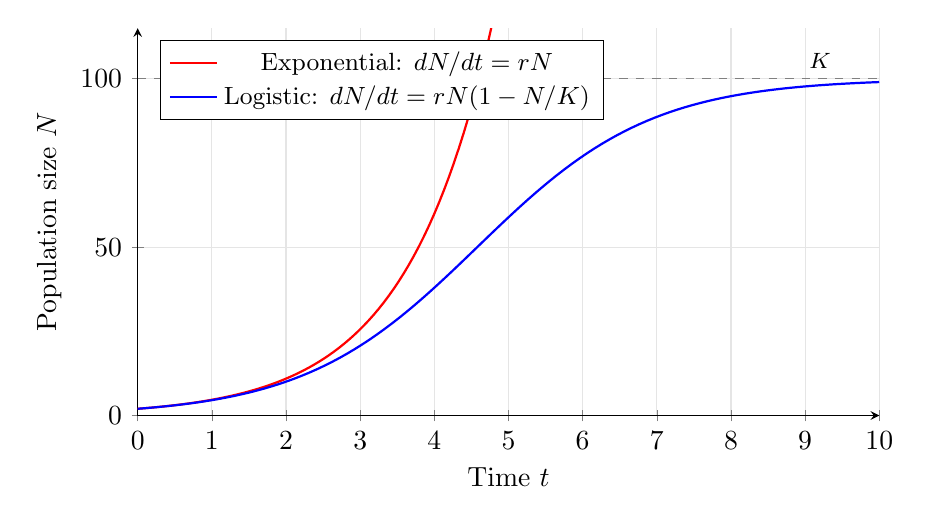
\begin{tikzpicture}
\begin{axis}[
  width=11cm, height=6.5cm,
  xlabel={Time $t$}, ylabel={Population size $N$},
  xmin=0, xmax=10, ymin=0, ymax=115,
  legend pos=north west, legend style={font=\small},
  axis lines=left, enlargelimits=false,
  grid=major, grid style={gray!20}
]
\addplot[thick, red, domain=0:5.35, samples=80] {2*exp(0.85*x)};
\addlegendentry{Exponential: $dN/dt = rN$}
\addplot[thick, blue, domain=0:10, samples=100] {100/(1+((100-2)/2)*exp(-0.85*x))};
\addlegendentry{Logistic: $dN/dt = rN(1-N/K)$}
\draw[dashed, gray] (axis cs:0,100) -- (axis cs:10,100) node[pos=0.92, above, black]{\footnotesize $K$};
\end{axis}
\end{tikzpicture}

\vspace{1mm}
\footnotesize The exponential curve (red) has no ceiling and accelerates indefinitely ($r=0.85$, truncated at $N=100$ purely so both curves share axes). The logistic curve (blue, same $r$, $K=100$) starts near-exponential while $N\ll K$, then decelerates as $N\to K$ due to the $(1-N/K)$ self-limitation term, and asymptotes at the carrying capacity.
\end{figbox}

\subsection{Problems with the logistic model, and the discrete Ricker model}
A key empirical problem flagged on the slides: when you actually plot the \emph{realized growth rate} against $N_t$ for real data, it is often \textbf{not} the clean, linearly-decreasing function that the logistic model assumes -- real "growth rate vs.\ density" curves are frequently humped or otherwise nonlinear. This motivates moving to discrete-time models with a more flexible (nonlinear, humped) density-dependence term. The key example used throughout the rest of the module is the \textbf{Ricker model}:
\[
n_{t+1} = n_t \exp\!\Big(r\big(1 - \tfrac{n_t}{k}\big)\Big),
\]
where, critically:
\begin{itemize}[leftmargin=1.5em]
\item $r$ (intrinsic growth rate) \textbf{determines the qualitative nature} of the dynamics (stable point vs.\ cycles vs.\ chaos);
\item $k$ (carrying capacity) only rescales population size and \textbf{does not affect the qualitative dynamics}.
\end{itemize}

\begin{exambox}
A very testable distinction: in the Ricker (and related) models, \emph{only the growth-rate parameter, not the carrying capacity, controls whether the population is stable, cyclic, or chaotic.} Carrying capacity is a "where," not a "what kind of," parameter.
\end{exambox}

\begin{figbox}[title={The Ricker model $N_{t+1}=N_t\,e^{\,r(1-N_t/K)}$: damped, cyclic, and chaotic regimes}]
\centering
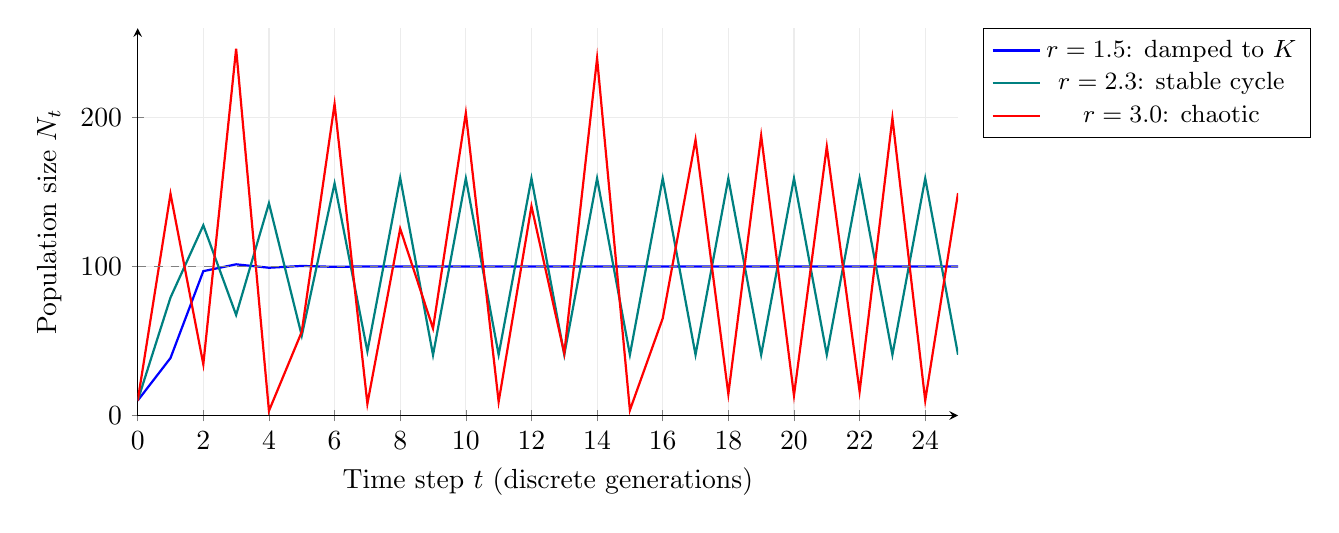
\begin{tikzpicture}
\begin{axis}[
  width=12cm, height=6.5cm,
  xlabel={Time step $t$ (discrete generations)}, ylabel={Population size $N_t$},
  xmin=0, xmax=25, ymin=0, ymax=260,
  legend pos=outer north east, legend style={font=\small},
  axis lines=left, enlargelimits=false,
  grid=major, grid style={gray!15}
]
\addplot[thick, blue, mark=none] coordinates {(0,10.0)(1,38.6)(2,96.9)(3,101.5)(4,99.2)(5,100.4)(6,99.8)(7,100.1)(8,100.0)(9,100.0)(10,100.0)(11,100.0)(12,100.0)(13,100.0)(14,100.0)(15,100.0)(16,100.0)(17,100.0)(18,100.0)(19,100.0)(20,100.0)(21,100.0)(22,100.0)(23,100.0)(24,100.0)(25,100.0)};
\addlegendentry{$r=1.5$: damped to $K$}
\addplot[thick, teal, mark=none] coordinates {(0,10.0)(1,79.2)(2,127.7)(3,67.5)(4,142.5)(5,53.6)(6,155.8)(7,43.1)(8,159.5)(9,40.6)(10,159.2)(11,40.8)(12,159.2)(13,40.8)(14,159.2)(15,40.8)(16,159.2)(17,40.8)(18,159.2)(19,40.8)(20,159.2)(21,40.8)(22,159.2)(23,40.8)(24,159.2)(25,40.8)};
\addlegendentry{$r=2.3$: stable cycle}
\addplot[thick, red, mark=none] coordinates {(0,10.0)(1,148.8)(2,34.4)(3,246.2)(4,3.1)(5,56.2)(6,209.1)(7,7.9)(8,125.4)(9,58.5)(10,203.0)(11,9.2)(12,140.5)(13,41.7)(14,239.8)(15,3.6)(16,65.2)(17,185.1)(18,14.4)(19,187.9)(20,13.5)(21,180.5)(22,16.1)(23,199.6)(24,10.1)(25,149.3)};
\addlegendentry{$r=3.0$: chaotic}
\draw[dashed, gray] (axis cs:0,100) -- (axis cs:25,100);
\end{axis}
\end{tikzpicture}

\vspace{1mm}
\footnotesize Real computed Ricker trajectories, same $K=100$ and $N_0=10$ throughout, only $r$ (intrinsic growth rate) differing. Exactly like the continuous logistic's discrete cousin: low $r$ settles smoothly onto $K$ (dashed line); moderate $r$ overshoots and undershoots $K$ in a stable oscillation; high $r$ produces fully chaotic, aperiodic fluctuations -- illustrating, in a single discrete-time model, the same qualitative route to complexity as the bifurcation diagram above.
\end{figbox}

\subsection{Behaviour of the Ricker map across increasing $r$: the road to chaos}
Iterating the Ricker map at increasing values of $r$ produces a well-known qualitative sequence, illustrated on the slides via time-series plots and summarized in a \textbf{bifurcation diagram} (population values plotted against $r$):

\begin{center}
\begin{tabularx}{\textwidth}{@{}l l X@{}}
\toprule
\textbf{Growth-rate regime} & \textbf{Example $r$} & \textbf{Qualitative long-run behaviour} \\
\midrule
Low & $r=1.3$ & \textbf{Stable point} -- the time series settles to one constant value. \\
Moderate & $r=2.3$ & \textbf{2-point limit cycle} -- population alternates between two fixed values every generation. \\
Higher & $r=2.5$ & \textbf{4-point limit cycle} -- a further period-doubling, alternating among 4 values. \\
High & $r=3.3$ & \textbf{Chaos} -- aperiodic, seemingly random fluctuations from a fully deterministic equation. \\
\bottomrule
\end{tabularx}
\end{center}

\begin{keybox}
\textbf{Reading a bifurcation diagram:} for a given value of $r$ (read along the $x$-axis), the number of distinct population values the system visits in the long run (read as the number of points plotted vertically above that $r$) \emph{is} the periodicity at that $r$ -- one point = stable equilibrium, two points = period-2 cycle, and so on, with the point-cloud eventually smearing into a continuum once chaos sets in. This period-doubling cascade (1 $\to$ 2 $\to$ 4 $\to$ 8 $\to \cdots \to$ chaos) as a single parameter is tuned is the central, generic phenomenon behind everything in this section (see the May 1976 paper summary below for the underlying mathematics).
\end{keybox}

\begin{figbox}[title={Bifurcation diagram: the period-doubling route to chaos (logistic map $x_{n+1}=r\,x_n(1-x_n)$)}]
\centering
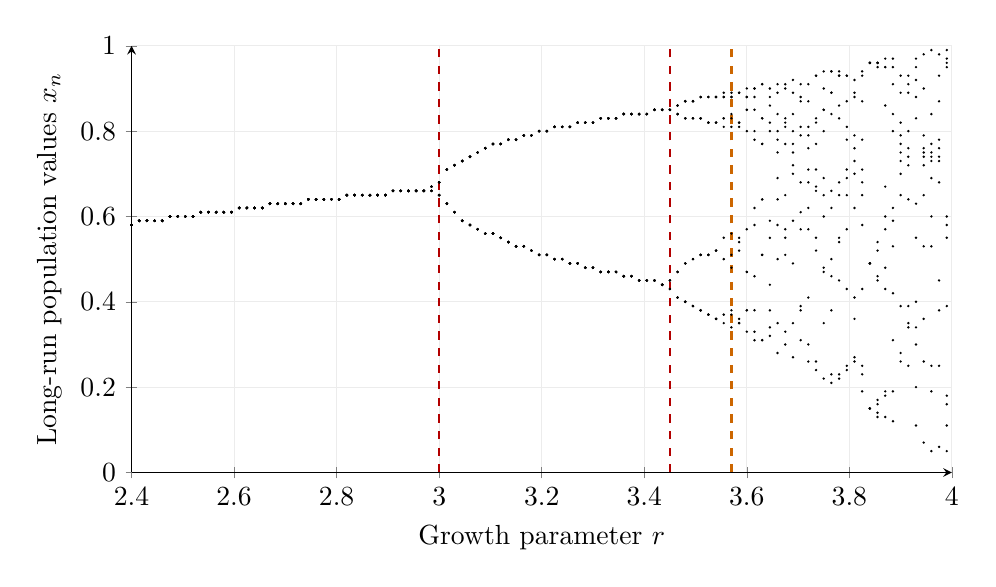
\begin{tikzpicture}
\begin{axis}[
  width=12cm, height=7cm,
  xlabel={Growth parameter $r$}, ylabel={Long-run population values $x_n$},
  xmin=2.4, xmax=4.0, ymin=0, ymax=1,
  axis lines=left, enlargelimits=false,
  grid=major, grid style={gray!15}
]
\addplot[only marks, mark=*, mark size=0.2pt, black] coordinates {
(2.400,0.58)(2.400,0.58)(2.400,0.58)(2.400,0.58)(2.400,0.58)(2.400,0.58)(2.400,0.58)(2.400,0.58)(2.400,0.58)(2.400,0.58)(2.400,0.58)(2.400,0.58)(2.415,0.59)(2.415,0.59)(2.415,0.59)(2.415,0.59)(2.415,0.59)(2.415,0.59)(2.415,0.59)(2.415,0.59)(2.415,0.59)(2.415,0.59)(2.415,0.59)(2.415,0.59)(2.430,0.59)(2.430,0.59)(2.430,0.59)(2.430,0.59)(2.430,0.59)(2.430,0.59)(2.430,0.59)(2.430,0.59)(2.430,0.59)(2.430,0.59)(2.430,0.59)(2.430,0.59)(2.445,0.59)(2.445,0.59)(2.445,0.59)(2.445,0.59)(2.445,0.59)(2.445,0.59)(2.445,0.59)(2.445,0.59)(2.445,0.59)(2.445,0.59)(2.445,0.59)(2.445,0.59)(2.460,0.59)(2.460,0.59)(2.460,0.59)(2.460,0.59)(2.460,0.59)(2.460,0.59)(2.460,0.59)(2.460,0.59)(2.460,0.59)(2.460,0.59)(2.460,0.59)(2.460,0.59)(2.475,0.60)(2.475,0.60)(2.475,0.60)(2.475,0.60)(2.475,0.60)(2.475,0.60)(2.475,0.60)(2.475,0.60)(2.475,0.60)(2.475,0.60)(2.475,0.60)(2.475,0.60)(2.490,0.60)(2.490,0.60)(2.490,0.60)(2.490,0.60)(2.490,0.60)(2.490,0.60)(2.490,0.60)(2.490,0.60)(2.490,0.60)(2.490,0.60)(2.490,0.60)(2.490,0.60)(2.505,0.60)(2.505,0.60)(2.505,0.60)(2.505,0.60)(2.505,0.60)(2.505,0.60)(2.505,0.60)(2.505,0.60)(2.505,0.60)(2.505,0.60)(2.505,0.60)(2.505,0.60)(2.520,0.60)(2.520,0.60)(2.520,0.60)(2.520,0.60)(2.520,0.60)(2.520,0.60)(2.520,0.60)(2.520,0.60)(2.520,0.60)(2.520,0.60)(2.520,0.60)(2.520,0.60)(2.535,0.61)(2.535,0.61)(2.535,0.61)(2.535,0.61)(2.535,0.61)(2.535,0.61)(2.535,0.61)(2.535,0.61)(2.535,0.61)(2.535,0.61)(2.535,0.61)(2.535,0.61)(2.550,0.61)(2.550,0.61)(2.550,0.61)(2.550,0.61)(2.550,0.61)(2.550,0.61)(2.550,0.61)(2.550,0.61)(2.550,0.61)(2.550,0.61)(2.550,0.61)(2.550,0.61)(2.565,0.61)(2.565,0.61)(2.565,0.61)(2.565,0.61)(2.565,0.61)(2.565,0.61)(2.565,0.61)(2.565,0.61)(2.565,0.61)(2.565,0.61)(2.565,0.61)(2.565,0.61)(2.580,0.61)(2.580,0.61)(2.580,0.61)(2.580,0.61)(2.580,0.61)(2.580,0.61)(2.580,0.61)(2.580,0.61)(2.580,0.61)(2.580,0.61)(2.580,0.61)(2.580,0.61)(2.595,0.61)(2.595,0.61)(2.595,0.61)(2.595,0.61)(2.595,0.61)(2.595,0.61)(2.595,0.61)(2.595,0.61)(2.595,0.61)(2.595,0.61)(2.595,0.61)(2.595,0.61)(2.610,0.62)(2.610,0.62)(2.610,0.62)(2.610,0.62)(2.610,0.62)(2.610,0.62)(2.610,0.62)(2.610,0.62)(2.610,0.62)(2.610,0.62)(2.610,0.62)(2.610,0.62)(2.625,0.62)(2.625,0.62)(2.625,0.62)(2.625,0.62)(2.625,0.62)(2.625,0.62)(2.625,0.62)(2.625,0.62)(2.625,0.62)(2.625,0.62)(2.625,0.62)(2.625,0.62)(2.640,0.62)(2.640,0.62)(2.640,0.62)(2.640,0.62)(2.640,0.62)(2.640,0.62)(2.640,0.62)(2.640,0.62)(2.640,0.62)(2.640,0.62)(2.640,0.62)(2.640,0.62)(2.655,0.62)(2.655,0.62)(2.655,0.62)(2.655,0.62)(2.655,0.62)(2.655,0.62)(2.655,0.62)(2.655,0.62)(2.655,0.62)(2.655,0.62)(2.655,0.62)(2.655,0.62)(2.670,0.63)(2.670,0.63)(2.670,0.63)(2.670,0.63)(2.670,0.63)(2.670,0.63)(2.670,0.63)(2.670,0.63)(2.670,0.63)(2.670,0.63)(2.670,0.63)(2.670,0.63)(2.685,0.63)(2.685,0.63)(2.685,0.63)(2.685,0.63)(2.685,0.63)(2.685,0.63)(2.685,0.63)(2.685,0.63)(2.685,0.63)(2.685,0.63)(2.685,0.63)(2.685,0.63)(2.700,0.63)(2.700,0.63)(2.700,0.63)(2.700,0.63)(2.700,0.63)(2.700,0.63)(2.700,0.63)(2.700,0.63)(2.700,0.63)(2.700,0.63)(2.700,0.63)(2.700,0.63)(2.715,0.63)(2.715,0.63)(2.715,0.63)(2.715,0.63)(2.715,0.63)(2.715,0.63)(2.715,0.63)(2.715,0.63)(2.715,0.63)(2.715,0.63)(2.715,0.63)(2.715,0.63)(2.730,0.63)(2.730,0.63)(2.730,0.63)(2.730,0.63)(2.730,0.63)(2.730,0.63)(2.730,0.63)(2.730,0.63)(2.730,0.63)(2.730,0.63)(2.730,0.63)(2.730,0.63)(2.745,0.64)(2.745,0.64)(2.745,0.64)(2.745,0.64)(2.745,0.64)(2.745,0.64)(2.745,0.64)(2.745,0.64)(2.745,0.64)(2.745,0.64)(2.745,0.64)(2.745,0.64)(2.760,0.64)(2.760,0.64)(2.760,0.64)(2.760,0.64)(2.760,0.64)(2.760,0.64)(2.760,0.64)(2.760,0.64)(2.760,0.64)(2.760,0.64)(2.760,0.64)(2.760,0.64)(2.775,0.64)(2.775,0.64)(2.775,0.64)(2.775,0.64)(2.775,0.64)(2.775,0.64)(2.775,0.64)(2.775,0.64)(2.775,0.64)(2.775,0.64)(2.775,0.64)(2.775,0.64)(2.790,0.64)(2.790,0.64)(2.790,0.64)(2.790,0.64)(2.790,0.64)(2.790,0.64)(2.790,0.64)(2.790,0.64)(2.790,0.64)(2.790,0.64)(2.790,0.64)(2.790,0.64)(2.805,0.64)(2.805,0.64)(2.805,0.64)(2.805,0.64)(2.805,0.64)(2.805,0.64)(2.805,0.64)(2.805,0.64)(2.805,0.64)(2.805,0.64)(2.805,0.64)(2.805,0.64)(2.820,0.65)(2.820,0.65)(2.820,0.65)(2.820,0.65)(2.820,0.65)(2.820,0.65)(2.820,0.65)(2.820,0.65)(2.820,0.65)(2.820,0.65)(2.820,0.65)(2.820,0.65)(2.835,0.65)(2.835,0.65)(2.835,0.65)(2.835,0.65)(2.835,0.65)(2.835,0.65)(2.835,0.65)(2.835,0.65)(2.835,0.65)(2.835,0.65)(2.835,0.65)(2.835,0.65)(2.850,0.65)(2.850,0.65)(2.850,0.65)(2.850,0.65)(2.850,0.65)(2.850,0.65)(2.850,0.65)(2.850,0.65)(2.850,0.65)(2.850,0.65)(2.850,0.65)(2.850,0.65)(2.865,0.65)(2.865,0.65)(2.865,0.65)(2.865,0.65)(2.865,0.65)(2.865,0.65)(2.865,0.65)(2.865,0.65)(2.865,0.65)(2.865,0.65)(2.865,0.65)(2.865,0.65)(2.880,0.65)(2.880,0.65)(2.880,0.65)(2.880,0.65)(2.880,0.65)(2.880,0.65)(2.880,0.65)(2.880,0.65)(2.880,0.65)(2.880,0.65)(2.880,0.65)(2.880,0.65)(2.895,0.65)(2.895,0.65)(2.895,0.65)(2.895,0.65)(2.895,0.65)(2.895,0.65)(2.895,0.65)(2.895,0.65)(2.895,0.65)(2.895,0.65)(2.895,0.65)(2.895,0.65)(2.910,0.66)(2.910,0.66)(2.910,0.66)(2.910,0.66)(2.910,0.66)(2.910,0.66)(2.910,0.66)(2.910,0.66)(2.910,0.66)(2.910,0.66)(2.910,0.66)(2.910,0.66)(2.925,0.66)(2.925,0.66)(2.925,0.66)(2.925,0.66)(2.925,0.66)(2.925,0.66)(2.925,0.66)(2.925,0.66)(2.925,0.66)(2.925,0.66)(2.925,0.66)(2.925,0.66)(2.940,0.66)(2.940,0.66)(2.940,0.66)(2.940,0.66)(2.940,0.66)(2.940,0.66)(2.940,0.66)(2.940,0.66)(2.940,0.66)(2.940,0.66)(2.940,0.66)(2.940,0.66)(2.955,0.66)(2.955,0.66)(2.955,0.66)(2.955,0.66)(2.955,0.66)(2.955,0.66)(2.955,0.66)(2.955,0.66)(2.955,0.66)(2.955,0.66)(2.955,0.66)(2.955,0.66)(2.970,0.66)(2.970,0.66)(2.970,0.66)(2.970,0.66)(2.970,0.66)(2.970,0.66)(2.970,0.66)(2.970,0.66)(2.970,0.66)(2.970,0.66)(2.970,0.66)(2.970,0.66)(2.985,0.67)(2.985,0.66)(2.985,0.67)(2.985,0.66)(2.985,0.67)(2.985,0.66)(2.985,0.67)(2.985,0.66)(2.985,0.67)(2.985,0.66)(2.985,0.67)(2.985,0.66)(3.000,0.68)(3.000,0.65)(3.000,0.68)(3.000,0.65)(3.000,0.68)(3.000,0.65)(3.000,0.68)(3.000,0.65)(3.000,0.68)(3.000,0.65)(3.000,0.68)(3.000,0.65)(3.015,0.71)(3.015,0.63)(3.015,0.71)(3.015,0.63)(3.015,0.71)(3.015,0.63)(3.015,0.71)(3.015,0.63)(3.015,0.71)(3.015,0.63)(3.015,0.71)(3.015,0.63)(3.030,0.72)(3.030,0.61)(3.030,0.72)(3.030,0.61)(3.030,0.72)(3.030,0.61)(3.030,0.72)(3.030,0.61)(3.030,0.72)(3.030,0.61)(3.030,0.72)(3.030,0.61)(3.045,0.73)(3.045,0.59)(3.045,0.73)(3.045,0.59)(3.045,0.73)(3.045,0.59)(3.045,0.73)(3.045,0.59)(3.045,0.73)(3.045,0.59)(3.045,0.73)(3.045,0.59)(3.060,0.74)(3.060,0.58)(3.060,0.74)(3.060,0.58)(3.060,0.74)(3.060,0.58)(3.060,0.74)(3.060,0.58)(3.060,0.74)(3.060,0.58)(3.060,0.74)(3.060,0.58)(3.075,0.75)(3.075,0.57)(3.075,0.75)(3.075,0.57)(3.075,0.75)(3.075,0.57)(3.075,0.75)(3.075,0.57)(3.075,0.75)(3.075,0.57)(3.075,0.75)(3.075,0.57)(3.090,0.76)(3.090,0.56)(3.090,0.76)(3.090,0.56)(3.090,0.76)(3.090,0.56)(3.090,0.76)(3.090,0.56)(3.090,0.76)(3.090,0.56)(3.090,0.76)(3.090,0.56)(3.105,0.77)(3.105,0.56)(3.105,0.77)(3.105,0.56)(3.105,0.77)(3.105,0.56)(3.105,0.77)(3.105,0.56)(3.105,0.77)(3.105,0.56)(3.105,0.77)(3.105,0.56)(3.120,0.77)(3.120,0.55)(3.120,0.77)(3.120,0.55)(3.120,0.77)(3.120,0.55)(3.120,0.77)(3.120,0.55)(3.120,0.77)(3.120,0.55)(3.120,0.77)(3.120,0.55)(3.135,0.78)(3.135,0.54)(3.135,0.78)(3.135,0.54)(3.135,0.78)(3.135,0.54)(3.135,0.78)(3.135,0.54)(3.135,0.78)(3.135,0.54)(3.135,0.78)(3.135,0.54)(3.150,0.78)(3.150,0.53)(3.150,0.78)(3.150,0.53)(3.150,0.78)(3.150,0.53)(3.150,0.78)(3.150,0.53)(3.150,0.78)(3.150,0.53)(3.150,0.78)(3.150,0.53)(3.165,0.79)(3.165,0.53)(3.165,0.79)(3.165,0.53)(3.165,0.79)(3.165,0.53)(3.165,0.79)(3.165,0.53)(3.165,0.79)(3.165,0.53)(3.165,0.79)(3.165,0.53)(3.180,0.79)(3.180,0.52)(3.180,0.79)(3.180,0.52)(3.180,0.79)(3.180,0.52)(3.180,0.79)(3.180,0.52)(3.180,0.79)(3.180,0.52)(3.180,0.79)(3.180,0.52)(3.195,0.80)(3.195,0.51)(3.195,0.80)(3.195,0.51)(3.195,0.80)(3.195,0.51)(3.195,0.80)(3.195,0.51)(3.195,0.80)(3.195,0.51)(3.195,0.80)(3.195,0.51)(3.210,0.80)(3.210,0.51)(3.210,0.80)(3.210,0.51)(3.210,0.80)(3.210,0.51)(3.210,0.80)(3.210,0.51)(3.210,0.80)(3.210,0.51)(3.210,0.80)(3.210,0.51)(3.225,0.81)(3.225,0.50)(3.225,0.81)(3.225,0.50)(3.225,0.81)(3.225,0.50)(3.225,0.81)(3.225,0.50)(3.225,0.81)(3.225,0.50)(3.225,0.81)(3.225,0.50)(3.240,0.81)(3.240,0.50)(3.240,0.81)(3.240,0.50)(3.240,0.81)(3.240,0.50)(3.240,0.81)(3.240,0.50)(3.240,0.81)(3.240,0.50)(3.240,0.81)(3.240,0.50)(3.255,0.81)(3.255,0.49)(3.255,0.81)(3.255,0.49)(3.255,0.81)(3.255,0.49)(3.255,0.81)(3.255,0.49)(3.255,0.81)(3.255,0.49)(3.255,0.81)(3.255,0.49)(3.270,0.82)(3.270,0.49)(3.270,0.82)(3.270,0.49)(3.270,0.82)(3.270,0.49)(3.270,0.82)(3.270,0.49)(3.270,0.82)(3.270,0.49)(3.270,0.82)(3.270,0.49)(3.285,0.82)(3.285,0.48)(3.285,0.82)(3.285,0.48)(3.285,0.82)(3.285,0.48)(3.285,0.82)(3.285,0.48)(3.285,0.82)(3.285,0.48)(3.285,0.82)(3.285,0.48)(3.300,0.82)(3.300,0.48)(3.300,0.82)(3.300,0.48)(3.300,0.82)(3.300,0.48)(3.300,0.82)(3.300,0.48)(3.300,0.82)(3.300,0.48)(3.300,0.82)(3.300,0.48)(3.315,0.83)(3.315,0.47)(3.315,0.83)(3.315,0.47)(3.315,0.83)(3.315,0.47)(3.315,0.83)(3.315,0.47)(3.315,0.83)(3.315,0.47)(3.315,0.83)(3.315,0.47)(3.330,0.83)(3.330,0.47)(3.330,0.83)(3.330,0.47)(3.330,0.83)(3.330,0.47)(3.330,0.83)(3.330,0.47)(3.330,0.83)(3.330,0.47)(3.330,0.83)(3.330,0.47)(3.345,0.83)(3.345,0.47)(3.345,0.83)(3.345,0.47)(3.345,0.83)(3.345,0.47)(3.345,0.83)(3.345,0.47)(3.345,0.83)(3.345,0.47)(3.345,0.83)(3.345,0.47)(3.360,0.84)(3.360,0.46)(3.360,0.84)(3.360,0.46)(3.360,0.84)(3.360,0.46)(3.360,0.84)(3.360,0.46)(3.360,0.84)(3.360,0.46)(3.360,0.84)(3.360,0.46)(3.375,0.84)(3.375,0.46)(3.375,0.84)(3.375,0.46)(3.375,0.84)(3.375,0.46)(3.375,0.84)(3.375,0.46)(3.375,0.84)(3.375,0.46)(3.375,0.84)(3.375,0.46)(3.390,0.84)(3.390,0.45)(3.390,0.84)(3.390,0.45)(3.390,0.84)(3.390,0.45)(3.390,0.84)(3.390,0.45)(3.390,0.84)(3.390,0.45)(3.390,0.84)(3.390,0.45)(3.405,0.84)(3.405,0.45)(3.405,0.84)(3.405,0.45)(3.405,0.84)(3.405,0.45)(3.405,0.84)(3.405,0.45)(3.405,0.84)(3.405,0.45)(3.405,0.84)(3.405,0.45)(3.420,0.85)(3.420,0.45)(3.420,0.85)(3.420,0.45)(3.420,0.85)(3.420,0.45)(3.420,0.85)(3.420,0.45)(3.420,0.85)(3.420,0.45)(3.420,0.85)(3.420,0.45)(3.435,0.85)(3.435,0.44)(3.435,0.85)(3.435,0.44)(3.435,0.85)(3.435,0.44)(3.435,0.85)(3.435,0.44)(3.435,0.85)(3.435,0.44)(3.435,0.85)(3.435,0.44)(3.450,0.85)(3.450,0.43)(3.450,0.85)(3.450,0.45)(3.450,0.85)(3.450,0.43)(3.450,0.85)(3.450,0.45)(3.450,0.85)(3.450,0.43)(3.450,0.85)(3.450,0.45)(3.465,0.86)(3.465,0.41)(3.465,0.84)(3.465,0.47)(3.465,0.86)(3.465,0.41)(3.465,0.84)(3.465,0.47)(3.465,0.86)(3.465,0.41)(3.465,0.84)(3.465,0.47)(3.480,0.87)(3.480,0.40)(3.480,0.83)(3.480,0.49)(3.480,0.87)(3.480,0.40)(3.480,0.83)(3.480,0.49)(3.480,0.87)(3.480,0.40)(3.480,0.83)(3.480,0.49)(3.495,0.87)(3.495,0.39)(3.495,0.83)(3.495,0.50)(3.495,0.87)(3.495,0.39)(3.495,0.83)(3.495,0.50)(3.495,0.87)(3.495,0.39)(3.495,0.83)(3.495,0.50)(3.510,0.88)(3.510,0.38)(3.510,0.83)(3.510,0.51)(3.510,0.88)(3.510,0.38)(3.510,0.83)(3.510,0.51)(3.510,0.88)(3.510,0.38)(3.510,0.83)(3.510,0.51)(3.525,0.88)(3.525,0.37)(3.525,0.82)(3.525,0.51)(3.525,0.88)(3.525,0.37)(3.525,0.82)(3.525,0.51)(3.525,0.88)(3.525,0.37)(3.525,0.82)(3.525,0.51)(3.540,0.88)(3.540,0.36)(3.540,0.82)(3.540,0.52)(3.540,0.88)(3.540,0.36)(3.540,0.82)(3.540,0.52)(3.540,0.88)(3.540,0.36)(3.540,0.82)(3.540,0.52)(3.555,0.88)(3.555,0.37)(3.555,0.83)(3.555,0.50)(3.555,0.89)(3.555,0.35)(3.555,0.81)(3.555,0.55)(3.555,0.88)(3.555,0.37)(3.555,0.83)(3.555,0.50)(3.570,0.88)(3.570,0.37)(3.570,0.83)(3.570,0.51)(3.570,0.89)(3.570,0.34)(3.570,0.81)(3.570,0.56)(3.570,0.88)(3.570,0.38)(3.570,0.84)(3.570,0.48)(3.585,0.89)(3.585,0.35)(3.585,0.82)(3.585,0.54)(3.585,0.89)(3.585,0.35)(3.585,0.81)(3.585,0.55)(3.585,0.89)(3.585,0.36)(3.585,0.82)(3.585,0.52)(3.600,0.88)(3.600,0.38)(3.600,0.85)(3.600,0.47)(3.600,0.90)(3.600,0.33)(3.600,0.80)(3.600,0.57)(3.600,0.88)(3.600,0.38)(3.600,0.85)(3.600,0.47)(3.615,0.90)(3.615,0.31)(3.615,0.78)(3.615,0.62)(3.615,0.85)(3.615,0.46)(3.615,0.90)(3.615,0.33)(3.615,0.80)(3.615,0.58)(3.615,0.88)(3.615,0.38)(3.630,0.91)(3.630,0.31)(3.630,0.77)(3.630,0.64)(3.630,0.83)(3.630,0.51)(3.630,0.91)(3.630,0.31)(3.630,0.77)(3.630,0.64)(3.630,0.83)(3.630,0.51)(3.645,0.90)(3.645,0.32)(3.645,0.80)(3.645,0.59)(3.645,0.88)(3.645,0.38)(3.645,0.86)(3.645,0.44)(3.645,0.90)(3.645,0.34)(3.645,0.82)(3.645,0.55)(3.660,0.80)(3.660,0.58)(3.660,0.89)(3.660,0.35)(3.660,0.84)(3.660,0.50)(3.660,0.91)(3.660,0.28)(3.660,0.75)(3.660,0.69)(3.660,0.78)(3.660,0.64)(3.675,0.81)(3.675,0.57)(3.675,0.90)(3.675,0.33)(3.675,0.82)(3.675,0.55)(3.675,0.91)(3.675,0.30)(3.675,0.77)(3.675,0.65)(3.675,0.83)(3.675,0.51)(3.690,0.80)(3.690,0.59)(3.690,0.89)(3.690,0.35)(3.690,0.84)(3.690,0.49)(3.690,0.92)(3.690,0.27)(3.690,0.72)(3.690,0.75)(3.690,0.70)(3.690,0.77)(3.705,0.68)(3.705,0.81)(3.705,0.57)(3.705,0.91)(3.705,0.31)(3.705,0.79)(3.705,0.61)(3.705,0.88)(3.705,0.39)(3.705,0.88)(3.705,0.38)(3.705,0.87)(3.720,0.26)(3.720,0.71)(3.720,0.76)(3.720,0.68)(3.720,0.81)(3.720,0.57)(3.720,0.91)(3.720,0.30)(3.720,0.79)(3.720,0.62)(3.720,0.87)(3.720,0.41)(3.735,0.82)(3.735,0.55)(3.735,0.93)(3.735,0.26)(3.735,0.71)(3.735,0.77)(3.735,0.66)(3.735,0.83)(3.735,0.52)(3.735,0.93)(3.735,0.24)(3.735,0.67)(3.750,0.69)(3.750,0.80)(3.750,0.60)(3.750,0.90)(3.750,0.35)(3.750,0.85)(3.750,0.48)(3.750,0.94)(3.750,0.22)(3.750,0.65)(3.750,0.85)(3.750,0.47)(3.765,0.46)(3.765,0.94)(3.765,0.23)(3.765,0.66)(3.765,0.84)(3.765,0.50)(3.765,0.94)(3.765,0.21)(3.765,0.62)(3.765,0.89)(3.765,0.38)(3.765,0.89)(3.780,0.55)(3.780,0.93)(3.780,0.23)(3.780,0.68)(3.780,0.83)(3.780,0.54)(3.780,0.94)(3.780,0.22)(3.780,0.65)(3.780,0.86)(3.780,0.45)(3.780,0.93)(3.795,0.57)(3.795,0.93)(3.795,0.25)(3.795,0.71)(3.795,0.78)(3.795,0.65)(3.795,0.87)(3.795,0.43)(3.795,0.93)(3.795,0.24)(3.795,0.69)(3.795,0.81)(3.810,0.26)(3.810,0.73)(3.810,0.76)(3.810,0.70)(3.810,0.79)(3.810,0.62)(3.810,0.89)(3.810,0.36)(3.810,0.88)(3.810,0.41)(3.810,0.92)(3.810,0.27)(3.825,0.19)(3.825,0.58)(3.825,0.93)(3.825,0.25)(3.825,0.71)(3.825,0.78)(3.825,0.65)(3.825,0.87)(3.825,0.43)(3.825,0.94)(3.825,0.23)(3.825,0.68)(3.840,0.96)(3.840,0.15)(3.840,0.49)(3.840,0.96)(3.840,0.15)(3.840,0.49)(3.840,0.96)(3.840,0.15)(3.840,0.49)(3.840,0.96)(3.840,0.15)(3.840,0.49)(3.855,0.96)(3.855,0.13)(3.855,0.45)(3.855,0.95)(3.855,0.17)(3.855,0.54)(3.855,0.96)(3.855,0.16)(3.855,0.52)(3.855,0.96)(3.855,0.14)(3.855,0.46)(3.870,0.67)(3.870,0.86)(3.870,0.48)(3.870,0.97)(3.870,0.13)(3.870,0.43)(3.870,0.95)(3.870,0.18)(3.870,0.57)(3.870,0.95)(3.870,0.19)(3.870,0.60)(3.885,0.80)(3.885,0.62)(3.885,0.91)(3.885,0.31)(3.885,0.84)(3.885,0.53)(3.885,0.97)(3.885,0.12)(3.885,0.42)(3.885,0.95)(3.885,0.19)(3.885,0.59)(3.900,0.28)(3.900,0.79)(3.900,0.65)(3.900,0.89)(3.900,0.39)(3.900,0.93)(3.900,0.26)(3.900,0.75)(3.900,0.73)(3.900,0.77)(3.900,0.70)(3.900,0.82)(3.915,0.35)(3.915,0.89)(3.915,0.39)(3.915,0.93)(3.915,0.25)(3.915,0.74)(3.915,0.76)(3.915,0.72)(3.915,0.80)(3.915,0.64)(3.915,0.91)(3.915,0.34)(3.930,0.34)(3.930,0.88)(3.930,0.40)(3.930,0.95)(3.930,0.20)(3.930,0.63)(3.930,0.92)(3.930,0.30)(3.930,0.83)(3.930,0.55)(3.930,0.97)(3.930,0.11)(3.945,0.53)(3.945,0.98)(3.945,0.07)(3.945,0.26)(3.945,0.75)(3.945,0.74)(3.945,0.76)(3.945,0.72)(3.945,0.79)(3.945,0.65)(3.945,0.90)(3.945,0.36)(3.960,0.25)(3.960,0.74)(3.960,0.75)(3.960,0.73)(3.960,0.77)(3.960,0.69)(3.960,0.84)(3.960,0.53)(3.960,0.99)(3.960,0.05)(3.960,0.19)(3.960,0.60)(3.975,0.38)(3.975,0.93)(3.975,0.25)(3.975,0.74)(3.975,0.76)(3.975,0.73)(3.975,0.78)(3.975,0.68)(3.975,0.87)(3.975,0.45)(3.975,0.98)(3.975,0.06)(3.990,0.60)(3.990,0.96)(3.990,0.16)(3.990,0.55)(3.990,0.99)(3.990,0.05)(3.990,0.18)(3.990,0.58)(3.990,0.97)(3.990,0.11)(3.990,0.39)(3.990,0.95)
};
\draw[dashed, red!70!black, thick] (axis cs:3.0,0) -- (axis cs:3.0,1) node[above]{\footnotesize $r{=}3.0$};
\draw[dashed, red!70!black, thick] (axis cs:3.45,0) -- (axis cs:3.45,1) node[above]{\footnotesize $r{=}3.45$};
\draw[dashed, orange!80!black, thick] (axis cs:3.57,0) -- (axis cs:3.57,1) node[above]{\footnotesize $r{\approx}3.57$};
\end{axis}
\end{tikzpicture}

\vspace{1mm}
\footnotesize Real computed bifurcation diagram (300 discarded transient iterations, then 12 plotted iterates per $r$ value). Below $r=3.0$: a single stable equilibrium. At $r=3.0$: first period-doubling bifurcation (equilibrium splits into a stable 2-cycle). At $r=3.45$: splits again into a 4-cycle. The period-doubling accelerates (period 8, 16, 32, \ldots) and accumulates at the Feigenbaum point $r\approx3.57$, beyond which the dynamics become chaotic (aperiodic, sensitive to initial conditions) -- visible here as the dense scattered band -- interspersed with narrow ``periodic windows'' (e.g.\ the clear period-3 window visible just above $r\approx3.83$).
\end{figbox}

\subsubsection*{Fractals: self-similarity in the bifurcation diagram}
Zooming into any one of the periodic "windows" within the chaotic region of a bifurcation diagram reveals a smaller copy of the same overall branching structure -- \textbf{self-similarity at multiple scales}, i.e.\ a \textbf{fractal}. (The slides note that the classic bifurcation-diagram image usually shown is generated from the closely related \emph{logistic} map $x_{t+1}=ax_t(1-x_t)$ rather than the Ricker map used elsewhere in this module, but the fractal principle is identical for both.)

\textit{Aside (non-technical, "fun" reading per the slides' own reading list, not examinable):} the reading list for this module includes an extract from Michael Crichton's \emph{Jurassic Park}, in which the character Ian Malcolm gives a pop-science explanation of \textbf{sensitive dependence on initial conditions (SDIC)} and fractals as hallmarks of chaotic systems -- useful as an intuition-builder (arbitrarily close starting points can diverge into totally different long-run trajectories) but not itself examinable content.

\subsection{Checking this against the real world: the Hassell model and a puzzling empirical result}
The natural next question: do real biological populations actually show this full range of behaviour -- stable points, limit cycles, chaos -- as theory predicts? The slides introduce the \textbf{Hassell model} (Hassell 1975, \emph{J.\ Anim.\ Ecol.} 44:283--295) as a flexible model fitted to real data:
\[
N_{t+1} = \lambda N_t (1+aN_t)^{-\beta},
\]
where $\lambda$ is the growth-rate parameter and $a,\beta$ jointly tune the density-dependent feedback (allowing both over- and under-compensating density dependence, unlike the single-shape Ricker curve).

\begin{papbox}[title={Paper Summary: Hassell, Lawton \& May (1976), \textit{J.\ Anim.\ Ecol.} 45:471--486 -- fitting the Hassell model to real insect populations}]
\textbf{Question:} Given that simple nonlinear population models can \emph{in principle} produce anything from stable points to chaos, what do \emph{real} insect populations actually do, empirically?

\textbf{Procedure:} Fitted the Hassell model (above) to time-series data from 24 natural insect populations, estimating $\lambda$ and $\beta$ for each and locating each population on the model's theoretical stability map ($\lambda$ vs.\ $\beta$).

\textbf{Key conclusion:} \textbf{22 of 24} populations exhibited \textbf{monotonic damping} -- the simplest, most boring possible stable dynamics -- with essentially none showing evidence of limit cycles or chaos. Headline takeaway as stated on the slides: \emph{"most natural populations exhibit relatively simple dynamics."}
\end{papbox}

This sets up the module's central puzzle, posed explicitly on the slides:
\begin{exambox}
\textbf{The paradox:} Simple mathematical models of population dynamics predict that populations \emph{could}, in principle, exhibit stable points, limit cycles, \emph{or} chaos (May 1976 -- see full paper summary below). This spurred many empirical hunts for chaos in real populations. Yet, except for one or two cases, \textbf{no real population has ever been convincingly shown to be chaotic} -- and Hassell et al.\ (1976) found overwhelmingly simple (monotonic damping) dynamics in real data. \textbf{So what's going on?} (This question is answered in two stages below: the "lattice effect," and Turchin \& Taylor's critique of Hassell et al.'s methodology.)
\end{exambox}

\begin{papbox}[title={Paper Summary: May (1976), \textit{Nature} 261:459--467 -- ``Simple Mathematical Models with Very Complicated Dynamics''}]
\textbf{What kind of paper this is:} a mathematical review/synthesis (not an empirical study), described on the course's own reading list as "the paper that (along with its 1974 sibling) ushered in the era of non-linear dynamics." There is therefore no single "procedure + conclusions" in the empirical sense; the paper's contribution is a unified mathematical account plus a call to apply it.

\textbf{Core content:} Considers the single first-order nonlinear difference equation $X_{t+1}=F(X_t)$ for a population with a "humped" density-dependence function $F$ (e.g.\ the logistic difference equation $X_{t+1}=aX_t(1-X_t)$, or the Ricker-type $X_{t+1}=X_t\exp[r(1-X_t)]$). May shows, graphically and algebraically, that as the steepness of the hump (tuned by a single parameter, e.g.\ $a$ or $r$) is increased:
\begin{itemize}[leftmargin=1.3em,nosep]
\item the single stable fixed point loses stability and \textbf{bifurcates} into a stable 2-point cycle, which itself later bifurcates into a 4-point cycle, then 8, 16, \ldots, $2^n$ -- an infinite \textbf{period-doubling cascade} that converges (for the logistic map, at parameter value $a_c\approx3.5700$);
\item beyond this accumulation point lies a \textbf{chaotic regime}: an infinite number of different periodic cycles coexist along with uncountably many genuinely \textbf{aperiodic} trajectories that never repeat, however long they are run (a phenomenon Li \& Yorke termed "chaos," and famously showed is guaranteed once a 3-point cycle appears -- "period three implies chaos");
\item in the chaotic regime, \textbf{arbitrarily close initial conditions eventually produce widely diverging trajectories} -- the same "butterfly effect" popularized (per Lorenz) in meteorology -- so that even a perfectly deterministic, perfectly parametrized model can be practically unpredictable in the long run;
\item the bifurcation structure is qualitatively \textbf{generic} to essentially any smooth, single-humped $F(X)$, not an artefact of the particular equation chosen.
\end{itemize}
\textbf{The empirical/applications section (directly relevant to the Hassell et al.\ puzzle above):} May shows a stability map (his Fig.\ 6, $\lambda$ vs.\ a density-dependence exponent $\beta$, using the very same Hassell-type model) plotting parameter estimates for 24 field-collected insect populations \emph{and} 4 laboratory populations. \textbf{Field populations cluster overwhelmingly in the stable-point region; laboratory populations show much more oscillatory/chaotic behaviour} -- tentatively attributed to the removal, in a lab setting, of natural mortality factors that would otherwise damp the dynamics. May explicitly flags this as tentative (small sample, technical difficulties in fitting single-species equations to what are really multi-species natural systems).
\end{papbox}

\subsection{Making the models more realistic: taming (or explaining away) chaos}
Given the paradox above, the module ends with \emph{two} distinct explanations for why real populations look far simpler than the theory allows -- one biological/structural, one methodological.

\subsubsection*{1. The lattice effect: organisms come in whole numbers}
Henson et al.\ (\emph{Science}, 19 October 2001) point out that population models like the ones above treat $N$ as a continuous real number, but real organisms are indivisible, integer-valued counts. Comparing an "unintegerized" (continuous) version of a chaotic model against an "integerized" (rounded-to-whole-numbers) version of the \emph{same} model: \textbf{chaos gives way to limit cycles or outright extinction} once integer constraints are imposed.

\begin{keybox}
\textbf{Why does integerisation kill chaos?} Deterministic chaos, by definition, requires trajectories that \emph{never} exactly repeat. But once population size is forced to be an integer \emph{and} the model structure imposes some finite upper bound on population size, the set of states the system can ever occupy is \textbf{finite}. A deterministic map acting on a finite state space must, sooner or later, revisit a state it has already visited -- and from that point on the trajectory is exactly periodic. So genuine (infinite-precision) chaos is structurally impossible once you integerise; you get periodicity (possibly with a very long period) instead. \textbf{Caveat:} this "lattice effect" only rules out truly \emph{deterministic} chaos -- it does not rule out long-period limit cycles, which can still look messy/quasi-random over any observable timescale.
\end{keybox}

\subsubsection*{2. Model complexity: are we just using models that are too simple to \emph{see} the chaos that is there?}
The second explanation directly re-examines Hassell et al.'s (1976) methodology, and is developed at length in the paired paper below.

\begin{papbox}[title={Paper Summary: Turchin \& Taylor (1992), \textit{Ecology} 73(1):289--305 -- ``Complex Dynamics in Ecological Time Series''}]
\textbf{Question:} Was Hassell et al.'s (1976) conclusion -- that real insect populations are overwhelmingly simple/stable -- actually correct, or was it an artefact of using an overly simple model to fit the data?

\textbf{Procedure:} Developed a \textbf{response-surface methodology (RSM)}: instead of assuming a fixed single-lag functional form, they fit the yearly per-capita population change $r_t$ as a flexible function of \emph{two} lagged population densities ($N_{t-1}$ and $N_{t-2}$, i.e.\ allowing \textbf{delayed density dependence}), including quadratic terms and a Box--Cox transformation for extra flexibility. This response-surface model was fit to \textbf{14 insect} and \textbf{22 vertebrate} long-term population time series, each classified by its reconstructed dynamical regime; classifications were cross-checked against each series' empirical \textbf{autocorrelation function (ACF)}, since periodic dynamics leave a distinctive ACF signature.

\textbf{Key conclusions:}
\begin{itemize}[leftmargin=1.3em,nosep]
\item Results were starkly different from Hassell et al.\ (1976): of the 14 insect populations, only \textbf{3} were classified as simple exponentially-stable, while the rest showed \textbf{damped oscillations (6), a limit cycle (1), quasiperiodic oscillations (2), or chaos (1)} -- i.e.\ the \emph{opposite} headline conclusion from Hassell et al.
\item The vertebrate datasets showed a similarly broad spectrum (though no confirmed chaos among the 22 vertebrate series).
\item Crucially, when Turchin \& Taylor deliberately \textbf{re-fit their own data using a simplified, single-lag model} (structurally similar to Hassell et al.'s), they recovered results very close to Hassell et al.'s original stable-dominated picture -- directly demonstrating that the earlier simple, stable conclusion was an artefact of insufficient model flexibility (missing time-lags and missing nonlinear/quadratic terms), not a true reflection of the underlying dynamics.
\item Headline conclusion, quoted directly on the course slides: \textbf{"Use of overly simple models for reconstructing endogenous dynamics from data may be biased in favor of finding stability."}
\item The paper's own visual analogy for why this happens: a genuinely complex, high-dimensional dynamical object can have a deceptively simple-looking \emph{low}-dimensional projection or shadow -- so inferring simple low-dimensional behaviour from data does not safely rule out a more complex underlying reality. (The slides flag this explicitly as "just an analogy," and separately note that this general lesson -- simple appearances can hide complex reality -- holds well beyond population dynamics.)
\end{itemize}
\end{papbox}

\begin{exambox}
\textbf{Likely essay-style question:} "Reconcile the apparently contradictory conclusions of Hassell et al.\ (1976) and Turchin \& Taylor (1992) about how common complex (cyclic/chaotic) dynamics are in nature." Expected answer structure: (i) both studies used real field/lab data, so the contradiction isn't about the data itself; (ii) Hassell et al.\ used a single-lag, comparatively inflexible functional form, which is mathematically biased toward finding stability, especially when the true system has delayed density dependence (very plausible biologically, e.g.\ via predator-prey or resource-consumer lags); (iii) Turchin \& Taylor's more flexible, multi-lag model recovers substantially more complex dynamics from much of the \emph{same kind} of data, and explicitly reproduce Hassell-et-al.-like results when they artificially strip their own model down to one lag -- directly showing the discrepancy is methodological, not biological. Combine this with the lattice-effect argument (organisms are discrete, imposing an upper bound on the achievable state space) as a \emph{second}, independent reason real long-term chaos is hard to observe even where the underlying continuous dynamics might in principle be chaotic.
\end{exambox}

\subsection{Summary comparison: the models of this section}
\begin{center}
\begin{tabularx}{\textwidth}{@{}l X X X@{}}
\toprule
\textbf{Model} & \textbf{Form} & \textbf{Density dependence} & \textbf{Possible long-run behaviour} \\
\midrule
Exponential & $N_t=N_0\lambda^t$ (or $N_0e^{rt}$) & None -- the "first law," baseline case & Unbounded growth/decline/stasis only \\
Continuous logistic (Verhulst--Pearl) & $\frac{1}{N}\frac{dN}{dt}=r(1-N/K)$ & Linear decline of realized growth rate with $N$ & Smooth approach to $K$ (no cycles -- it's continuous-time) \\
Ricker (discrete) & $n_{t+1}=n_t e^{\,r(1-n_t/k)}$ & Nonlinear/humped; strength tuned by $r$ alone & Stable pt.\ $\to$ 2-pt.\ $\to$ 4-pt.\ cycle $\to$ chaos as $r$ increases \\
Hassell & $N_{t+1}=\lambda N_t(1+aN_t)^{-\beta}$ & Flexible over-/under-compensation via $a,\beta$ & Same qualitative spectrum as Ricker; fitted directly to 24 field populations by Hassell et al.\ (1976) \\
\bottomrule
\end{tabularx}
\end{center}

\newpage

% =====================================================================
\section{Competition: Exclusion, Coexistence, and the Special Case of Invasive Species}
% =====================================================================

\subsection{Defining competition}
Competition is defined on the slides as \textbf{"any use or defense of a resource by one individual that reduces the availability of that resource to other individuals."} In words: two individuals (or populations) use, or seek to use, the same limited resource, to the detriment of one or both. Two kinds are distinguished by \emph{who} is competing:

\begin{center}
\begin{tabularx}{\textwidth}{@{}l X@{}}
\toprule
\textbf{Type} & \textbf{Definition / example} \\
\midrule
Intraspecific competition & Between members of the \emph{same} species. Already covered implicitly earlier in the course via density-dependent reduction in population growth rate (logistic-type models); another major example is competition for mates. \\
Interspecific competition & Between members of \emph{different} species, for the same limiting resource. Features: it is a \textbf{nontrophic} interaction (neither species eats the other -- this distinguishes it from predation), and it reduces the population growth rate or equilibrium population size of at least one, often both, of the populations. If two species genuinely do not affect each other, there is, by definition, no competition between them. \\
\bottomrule
\end{tabularx}
\end{center}

\begin{exambox}
A quick way to distinguish competition from predation on an exam: competition is \emph{nontrophic} (no one is eaten), whereas predation is trophic. Both can reduce a population's growth rate, so "reduces growth rate of the other species" alone is not sufficient to identify competition -- the absence of consumption is the key extra criterion.
\end{exambox}

\subsection{Early experimental and theoretical results on interspecific competition}
\subsubsection*{Gause's principle of competitive exclusion}
Gause's classic experiments (using \emph{Paramecium} species, discussed further below) established the \textbf{competitive exclusion principle}: \textbf{no two species with exactly the same niche can co-exist} -- one will always eventually exclude the other.

\subsubsection*{Tilman's resource-competition experiments and the R* rule}
Tilman et al. (1981) extended this experimentally using algal species competing for a single limiting nutrient, confirming that \textbf{two species cannot coexist indefinitely on a single limiting resource}. This was formalized as the \textbf{R* rule} (Tilman, 1982) for exploitative competition (competition mediated purely through consumption of a shared resource, not direct interference):

\begin{keybox}
\textbf{R* rule:} When two or more species are limited by the same single resource, the species that can maintain a \emph{positive} per-capita growth rate at the \emph{lowest} resource level ($R^{*}$) will competitively exclude all other species -- because it can keep growing (or at least not decline) even after it has drawn the shared resource down to a level at which its competitors can no longer sustain themselves.
\end{keybox}

\begin{figbox}[title={Tilman's $R^*$ rule for exploitative competition}]
\centering
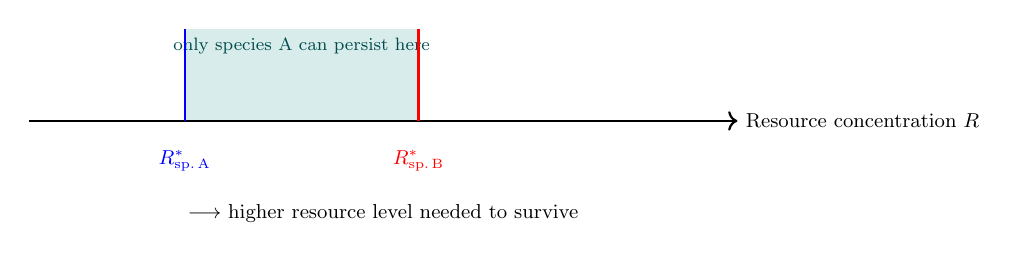
\begin{tikzpicture}[scale=0.9, every node/.style={scale=0.9}, transform shape]
\fill[teal!15] (2.2,0) rectangle (5.5,1.3);
\node[teal!60!black] at (3.85,1.05) {\footnotesize only species A can persist here};
\draw[->, thick] (0,0) -- (10,0) node[right]{\small Resource concentration $R$};
\draw[thick, blue] (2.2,0) -- (2.2,1.3);
\node[blue, below] at (2.2,-0.3) {\small $R^*_{\text{sp.\,A}}$};
\draw[thick, red] (5.5,0) -- (5.5,1.3);
\node[red, below] at (5.5,-0.3) {\small $R^*_{\text{sp.\,B}}$};
\node at (5.0,-1.3) {\small $\longrightarrow$ higher resource level needed to survive};
\end{tikzpicture}

\vspace{4mm}
\footnotesize $R^*$ = the resource concentration at which a species' population growth exactly balances its mortality (its own break-even resource level). Whichever species can drive the shared limiting resource down furthest -- i.e.\ has the \textbf{lower} $R^*$ -- can persist on the scraps the other species cannot survive on, and competitively excludes it at equilibrium (species A wins here, since $R^*_A<R^*_B$: A can keep growing all the way down to the shaded zone, where B's minimum requirement is already unmet). This single-number rule generalizes the graphical isocline logic in the figure above to resource-mediated (exploitative) competition for one limiting resource.
\end{figbox}

\subsection{The Lotka--Volterra competition model}
The mathematical formalization of two-species competition extends the logistic growth equation (Topic 3) by adding a term for the competitive effect of the other species:
\[
\frac{dN_1}{dt} = \frac{r_1 N_1 (K_1 - N_1 - \alpha_{12}N_2)}{K_1}, \qquad
\frac{dN_2}{dt} = \frac{r_2 N_2 (K_2 - N_2 - \alpha_{21}N_1)}{K_2},
\]
where $\alpha_{12}$ is the \textbf{competition coefficient} -- it converts individuals of species 2 into "resource-equivalent" units of species 1, i.e.\ it denotes the effect on species 1's growth rate of adding one individual of species 2 (and symmetrically for $\alpha_{21}$).

\begin{keybox}
\textbf{Reading the competition coefficients:} $\alpha_{12} > 1$ means each individual of species 2 suppresses species 1's growth \emph{more} than an additional individual of species 1 itself would (interspecific competition stronger than intraspecific); $\alpha_{12} < 1$ means the reverse. This asymmetry between $\alpha_{12}$ and $\alpha_{21}$ is what produces the varied outcomes below, rather than a single universal result.
\end{keybox}

\subsubsection*{Graphical analysis: zero-growth isoclines}
Setting $dN_1/dt = 0$ and $dN_2/dt = 0$ gives each species' \textbf{zero-growth isocline} -- the line in $(N_1,N_2)$ space along which that species' population is momentarily stationary. Plotting both isoclines on the same axes and examining where/how they cross yields four qualitatively distinct outcomes:

\begin{center}
\begin{tabularx}{\textwidth}{@{}l X@{}}
\toprule
\textbf{Outcome} & \textbf{Geometric condition (isoclines don't cross, or cross how)} \\
\midrule
Species 1 always wins & Species 1's isocline lies entirely outside species 2's -- species 1 can tolerate more of species 2 than species 2 can tolerate of species 1 across the whole range. \\
Species 2 always wins & Symmetric case with the isoclines' roles reversed. \\
Stable (coexistence) equilibrium & Isoclines cross, and each species inhibits itself more than it inhibits the other ($\alpha_{12}, \alpha_{21}$ both comparatively weak) -- the crossing point is a stable node the system converges to regardless of starting densities. \\
Unstable equilibrium (founder control) & Isoclines cross the opposite way -- each species inhibits the \emph{other} more than itself ($\alpha_{12},\alpha_{21}$ both comparatively strong) -- whichever species starts with the numerical advantage wins; the crossing point is unstable, and the outcome depends on initial conditions. \\
\bottomrule
\end{tabularx}
\end{center}

\begin{figbox}[title={Lotka--Volterra competition: zero-growth isoclines and the four qualitative outcomes}]
\centering
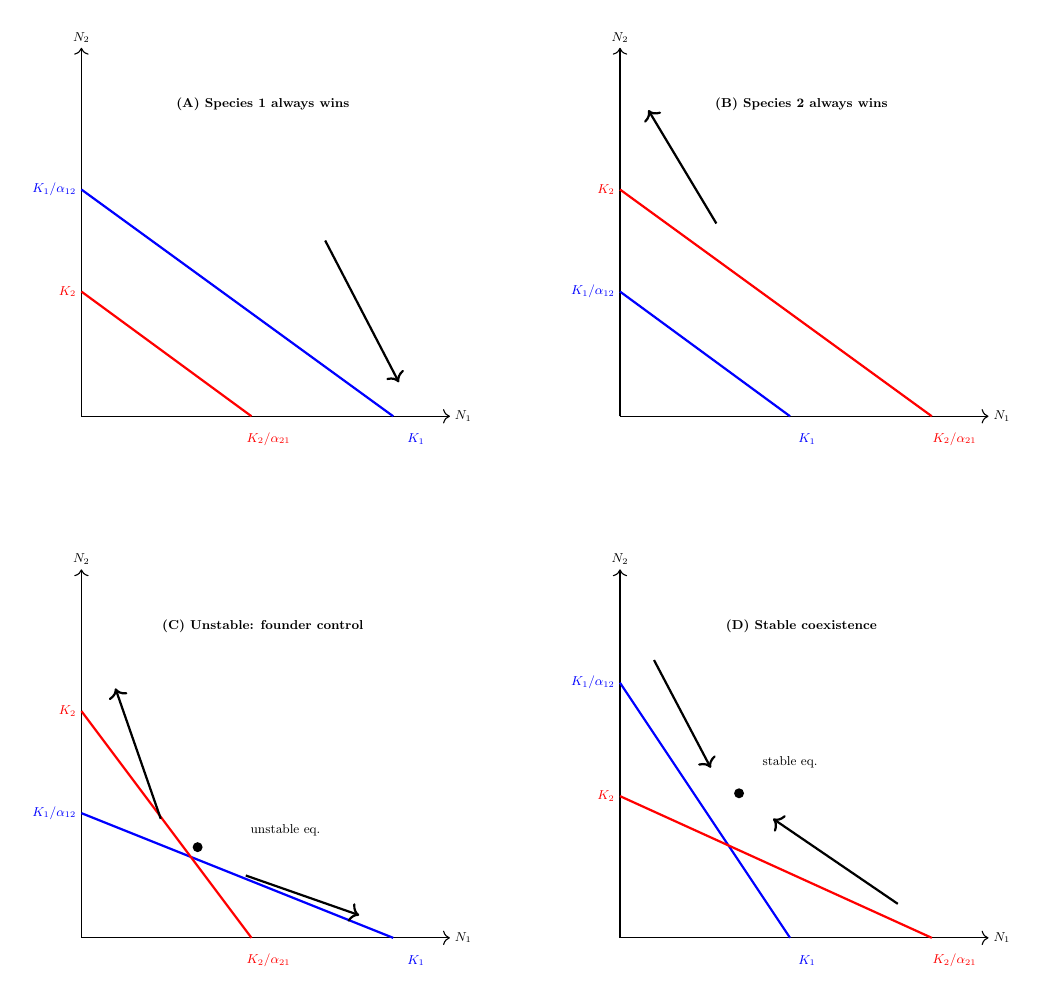
\begin{tikzpicture}[scale=0.72, every node/.style={scale=0.72}, transform shape]
\begin{scope}[xshift=0cm, yshift=9.2cm]
\draw[->] (0,0) -- (6.5,0) node[right]{\small $N_1$};
\draw[->] (0,0) -- (0,6.5) node[above]{\small $N_2$};
\draw[thick, blue] (5.5,0) -- (0,4) node[left]{\small $K_1/\alpha_{12}$};
\node[blue] at (5.9,-0.4) {\small $K_1$};
\draw[thick, red] (3,0) -- (0,2.2) node[left]{\small $K_2$};
\node[red] at (3.3,-0.4) {\small $K_2/\alpha_{21}$};
\draw[->, thick, black] (4.3,3.1) -- (5.6,0.6);
\node at (3.2,5.5) {\small \textbf{(A) Species 1 always wins}};
\end{scope}
\begin{scope}[xshift=9.5cm, yshift=9.2cm]
\draw[->] (0,0) -- (6.5,0) node[right]{\small $N_1$};
\draw[->] (0,0) -- (0,6.5) node[above]{\small $N_2$};
\draw[thick, blue] (3,0) -- (0,2.2) node[left]{\small $K_1/\alpha_{12}$};
\node[blue] at (3.3,-0.4) {\small $K_1$};
\draw[thick, red] (5.5,0) -- (0,4) node[left]{\small $K_2$};
\node[red] at (5.9,-0.4) {\small $K_2/\alpha_{21}$};
\draw[->, thick, black] (1.7,3.4) -- (0.5,5.4);
\node at (3.2,5.5) {\small \textbf{(B) Species 2 always wins}};
\end{scope}
\begin{scope}[xshift=0cm, yshift=0cm]
\draw[->] (0,0) -- (6.5,0) node[right]{\small $N_1$};
\draw[->] (0,0) -- (0,6.5) node[above]{\small $N_2$};
\draw[thick, blue] (5.5,0) -- (0,2.2) node[left]{\small $K_1/\alpha_{12}$};
\node[blue] at (5.9,-0.4) {\small $K_1$};
\draw[thick, red] (3,0) -- (0,4) node[left]{\small $K_2$};
\node[red] at (3.3,-0.4) {\small $K_2/\alpha_{21}$};
\fill (2.05,1.6) circle (2.5pt);
\node at (3.6,1.9) {\small unstable eq.};
\draw[->, thick, black] (1.4,2.1) -- (0.6,4.4);
\draw[->, thick, black] (2.9,1.1) -- (4.9,0.4);
\node at (3.2,5.5) {\small \textbf{(C) Unstable: founder control}};
\end{scope}
\begin{scope}[xshift=9.5cm, yshift=0cm]
\draw[->] (0,0) -- (6.5,0) node[right]{\small $N_1$};
\draw[->] (0,0) -- (0,6.5) node[above]{\small $N_2$};
\draw[thick, blue] (3,0) -- (0,4.5) node[left]{\small $K_1/\alpha_{12}$};
\node[blue] at (3.3,-0.4) {\small $K_1$};
\draw[thick, red] (5.5,0) -- (0,2.5) node[left]{\small $K_2$};
\node[red] at (5.9,-0.4) {\small $K_2/\alpha_{21}$};
\fill (2.1,2.55) circle (2.5pt);
\node at (3.0,3.1) {\small stable eq.};
\draw[->, thick, black] (0.6,4.9) -- (1.6,3.0);
\draw[->, thick, black] (4.9,0.6) -- (2.7,2.1);
\node at (3.2,5.5) {\small \textbf{(D) Stable coexistence}};
\end{scope}
\end{tikzpicture}

\vspace{1mm}
\footnotesize Blue line = species 1's zero-growth isocline ($dN_1/dt=0$); red line = species 2's isocline ($dN_2/dt=0$). Whichever species' isocline lies entirely \emph{outside} the other's (panels A, B) always wins -- it can still grow even at the point where the loser's growth has already stopped. When the isoclines cross (panels C, D), the outcome depends on whether each species inhibits the \emph{other} more or less than it inhibits \emph{itself}: if each species' own carrying-capacity intercept is \emph{inside} the other's line (each is a weaker self-limiter than competitor) $\to$ unstable equilibrium, whoever has the early numerical edge excludes the other (panel C, ``founder control''/priority effect). If each species' own intercept is \emph{outside} the other's line (each limits itself more than it limits its rival) $\to$ stable coexistence at the interior crossing point (panel D).
\end{figbox}

\begin{exambox}
\textbf{Main message from the L--V competition model (stated explicitly on the slides):} in \textbf{3 out of 4} of the qualitative parameter combinations, the model predicts that one species will drive the other to extinction -- broadly consistent with at least some experimental results (e.g.\ Gause, Tilman). Only the specific case of mutual weak interspecific competition (each species limiting itself more than it limits its rival) permits stable coexistence. The instructor's own framing of "what about real life?" -- answer: "it is complicated" -- is a deliberate segue into the rest of the topic (invasive species as a stark real-world confirmation of competitive exclusion, versus widespread real-world coexistence explained via niche partitioning).
\end{exambox}

\subsection{The case of the super-competitors: invasive species}
Invasive species are presented as a vivid, real-world confirmation of the competitive-exclusion logic above: a species introduced into a new range often out-competes native species for shared resources, sometimes catastrophically. The slides use a local case study: the \textbf{2018 and 2019 Kerala floods}, after which large invasive fish -- \emph{Arapaima} (up to $\sim$200 kg) and alligator gar (up to $\sim$137 kg) -- began appearing in Kerala's rivers, most likely escapees from the aquarium/ornamental-fish trade that the floodwaters released into the wild. A 2021 survey of 44 rivers and 53 reservoirs in Kerala found the state's waters host \textbf{28 alien fish species and 4 alien aquatic weed/macrophyte species}, of which \textbf{7 fish species have already established self-sustaining natural populations}; the two dominant pathways of introduction identified were the \textbf{aquarium trade} and \textbf{aquaculture}.

\begin{papbox}[title={Slide case-study citation: Raj et al. (2021), \textit{Aquatic Ecosystem Health \& Management} 24(2), 64--75 -- ``Distribution of alien invasive species in aquatic ecosystems of the southern Western Ghats, India''}]
Cited directly on the slides as the source of the Kerala survey statistics above (28 alien fish species, 4 alien macrophytes, 7 established fish species across 44 rivers/53 reservoirs surveyed). Treat this as a data citation to remember (the numbers themselves are the exam-relevant content) rather than a paper requiring a full procedure/conclusion writeup.
\end{papbox}

\subsubsection*{The human angle: living with (and using) invasive species}
Beyond eradication, the slides highlight community-level responses that turn an invasive species into an economic resource -- most notably \textbf{water hyacinth} (an aggressively invasive floating aquatic weed) being converted into a livelihood material in India: e.g.\ the Kottapuram Integrated Development Society (KIDS) in Kerala trains women in Paravur to make crafts from water hyacinth fiber; the Assam State Rural Livelihoods Mission produces mats/baskets/handicrafts from it; and in West Bengal it is woven into Shantipur cotton sarees (in a 30:70 hyacinth:cotton blend). Two further case studies are flagged on the slides as \emph{self-study} (not covered in class detail, so not elaborated here): \textbf{Asian carp} in North American waterways, and \textbf{\emph{Caulerpa taxifolia}} (an invasive marine alga).

\subsection{The other paper: Sakai et al. (2001) on the population biology of invasive species}
This is the sole \emph{Paper}-tier reference on the topic's reading-material slide (alongside Molles Ch.\ 13 as textbook-level Mandatory reading, which is skipped here per the project's standing rule since the lecture slides above are already self-contained on the core competition concepts). It is a broad synthesis/review article, not a single experiment, so the summary below is organized by theme rather than by a single procedure.

\begin{papbox}[title={Paper Summary: Sakai, Allendorf, Holt et al. (2001), \textit{Annu. Rev. Ecol. Syst.} 32:305--332 -- ``The Population Biology of Invasive Species''}]
\textbf{Scope:} A review arguing that \textbf{population biology} (ecology $+$ genetics $+$ evolution together) is the right lens for understanding \emph{why} some introduced species become invasive and others do not, and for guiding management. The invasion process is framed as a sequence of stages, each raising its own population-biology questions: (a) \textbf{introduction} into a new habitat, (b) \textbf{initial colonization and establishment}, and (c) \textbf{subsequent dispersal/range expansion}.

\textbf{Key themes and conclusions:}
\begin{itemize}[leftmargin=1.3em,nosep]
\item \emph{Life-history predictors are useful but imperfect.} Baker's classic "ideal weed" traits (sexual + asexual reproduction, rapid growth to maturity, high phenotypic plasticity, tolerance of environmental heterogeneity) and cross-taxa patterns (r-selected life histories: short generation time, high fecundity, high growth rate; strong dispersal ability) correlate with invasiveness, but many successful invaders lack most of these traits -- generalizations break down and taxon-/habitat-specific analysis is often needed.
\item \emph{Genetic bottlenecks vs.\ multiple introductions.} A single small founding population typically loses genetic diversity (bottleneck via drift), which can cause inbreeding depression and limits future adaptive potential. \textbf{Multiple, repeated introductions} (often from different source populations) can counteract this by restoring genetic variation -- consistent with the empirical pattern that repeated introductions are strongly associated with eventual invasion success (e.g.\ European starling, house sparrow in North America).
\item \emph{Lag times} between initial colonization and rapid spread are common, and may reflect ordinary exponential-growth lag dynamics \emph{and/or} the time required for adaptive evolution to overcome initial genetic/ecological constraints -- the paper stresses these are not mutually exclusive and disentangling them is an open research question.
\item \emph{Range expansion involves a genetic tension:} high dispersal brings gene flow that supplies genetic variation at the invasion front, but the same gene flow (especially from a large central population) can swamp locally advantageous alleles and thereby \emph{limit} adaptation and further spread (Kirkpatrick \& Barton 1997 models).
\item \emph{Invasibility of communities is an emergent, context-dependent property} -- it depends jointly on the invader's traits, the resident species' traits (competitive ability, disturbance resistance), and community-level factors (disturbance regime, diversity/functional redundancy, trophic structure). Empirical support for "diverse communities resist invasion better" is mixed. Reduced top-down/enemy pressure in the new range (missing predators, pathogens, competitors) is repeatedly cited as an ecological reason invasive species can flourish -- directly connecting to the "why so few negative interactions constrain the invader" logic behind the L--V/R* results above.
\item \emph{Species interactions can themselves evolve rapidly} in response to an invasion, in either direction: an evolved response in a native species can either strengthen community resistance to further invasion, or (via disruption of existing interaction networks) make the community \emph{more} susceptible -- e.g.\ evolved antipredator behavior in invertebrates following introduction of brown trout in a New Zealand river altered algal biomass community-wide.
\item \textbf{Overall conclusion:} because ecological and evolutionary/genetic processes interact throughout every stage of invasion, effective prediction and management of invasive species requires combining tools from both traditions (molecular genetic markers, quantitative genetics, and population/range-expansion models together), not ecology or genetics alone.
\end{itemize}
\end{papbox}

\begin{exambox}
Likely conceptual link to draw explicitly: the L--V/R* theoretical prediction that \textbf{competitive exclusion is common} is empirically borne out in a striking way by invasive species (a "natural experiment" where a highly competitive newcomer is suddenly added to a community) -- Sakai et al.'s review is essentially cataloguing \emph{why} some species turn out to be that superior competitor (life history $+$ reduced natural enemies $+$ genetic factors) and what determines whether the invaded community can resist them.
\end{exambox}

\subsection{The case of the competition-avoiders: how coexistence actually happens}
Despite the exclusion result above, many species with apparently similar niches \emph{do} coexist in nature. Resolving this requires first defining the \textbf{ecological niche} precisely.

\subsubsection*{What is a niche?}
The niche is introduced as an \textbf{$n$-dimensional hypervolume}: each relevant environmental or resource axis (temperature, salinity, food type, pH, etc.) is one dimension, and a species' niche is the region of that multidimensional space within which it can persist. The slides illustrate this concretely with 1-D (temperature range for net photosynthesis in alpine plants), 2-D (temperature $\times$ salinity tolerance for sand-shrimp egg-bearing females), and 3-D (temperature $\times$ pH $\times$ food availability for an aquatic organism) examples.

Two complementary formal definitions of niche are given, associated with different historical traditions in ecology:
\begin{center}
\begin{tabularx}{\textwidth}{@{}l X@{}}
\toprule
\textbf{Definition} & \textbf{Content} \\
\midrule
Population-persistence niche (Hutchinson) & "A quantitative description of the range of environmental conditions that allow a population to persist" -- where \emph{persist} means having a positive growth rate. This is the classic $n$-dimensional-hypervolume formulation. \\
Resource-utilization niche (McArthur \& Levins) & Focuses not on tolerance limits but on \emph{what a population actually does} -- specifically, how it uses resources along axes such as habitat (micro-/macrohabitat), food type (size, hardness), and time (daily/seasonal activity pattern). \\
\bottomrule
\end{tabularx}
\end{center}

\begin{exambox}
The slides quote N.G. Hairston Jr.\ (1995): "Ecology's love-hate relationship with the niche concept has been long and not especially pretty" -- a useful line to remember if asked to comment critically on the niche concept's history; it signals that the niche is a genuinely useful but historically contested and imprecisely-agreed-upon idea, not a single settled definition.
\end{exambox}

\subsubsection*{Coexistence via niche partitioning}
The general resolution: species can coexist \textbf{if their niches are sufficiently separated/partitioned} along one or more axes, so that they are no longer competing for exactly the same limiting resource. The slides distinguish several concrete mechanisms of \textbf{resource partitioning}, each illustrated with a classic example:

\begin{center}
\begin{tabularx}{\textwidth}{@{}l X@{}}
\toprule
\textbf{Mechanism} & \textbf{Classic example (from slides)} \\
\midrule
Spatial partitioning & \emph{Gause's Paramecium experiment}: \textit{P.\ caudatum} and \textit{P.\ bursaria} coexist in the same culture vessel because the former feeds in the top layers and the latter in the bottom layers -- vertical spatial separation within an apparently uniform habitat. \emph{Connell's barnacles} (\textit{Chthamalus} vs.\ \textit{Balanus} on a rocky shore) show a sharp vertical zonation on intertidal rocks: this is the classic case where the two species' \emph{fundamental} niches (what each could tolerate physiologically) overlap broadly, but their \emph{realized} niches (what they actually occupy once competition is allowed to play out) are separated -- \textit{Balanus} competitively excludes \textit{Chthamalus} from the lower, wetter zone it could otherwise also tolerate, while \textit{Chthamalus} persists in the upper zone because it can tolerate desiccation stress that excludes \textit{Balanus} there. (This fundamental-vs-realized-niche distinction is the standard textbook lesson drawn from Connell's experiment and is worth stating explicitly even though the slide itself poses it only as an open question.) \\
Temporal partitioning & \emph{Spiny mice in Israeli deserts}: the common spiny mouse (\textit{Acomys cahirinus}, normally nocturnal) and the golden spiny mouse (\textit{A.\ russatus}, normally diurnal) coexist despite overlapping habitat, food preference, and breeding season -- separated instead by activity time. When the common (nocturnal) species was experimentally removed, the golden species shifted to become nocturnal itself, directly demonstrating that the diurnal habit was an evolved/plastic response to \emph{avoid} competition with the numerically dominant nocturnal species, not a fixed trait (Shkolnik 1971; Kronfeld-Schor \& Dayan 1999). \\
Morphological partitioning & \textbf{Character displacement}: closely related species show \emph{greater} difference in a character (e.g.\ beak size, body size) where they occur \emph{together} (sympatry) than where they occur separately (allopatry) -- interpreted as evolutionary divergence driven by selection to reduce resource-use overlap where competition would otherwise be strongest. \\
Conditional niche differentiation & \emph{Thomas Park's \textit{Tribolium} flour-beetle experiments} (1954, 1962): pitting \textit{T.\ confusum} against \textit{T.\ castaneum} across a grid of temperature and humidity conditions showed that \emph{which} species wins depends on the physical conditions (e.g.\ one species dominates at $34^{\circ}$C/70\% RH, the other at $24^{\circ}$C/30\% RH) -- i.e.\ the outcome of competition is conditional on the abiotic environment, not fixed by the species pair alone. \\
\bottomrule
\end{tabularx}
\end{center}

\begin{exambox}
Two closely related, high-value exam takeaways from Park's flour-beetle work, stated directly on the slides: (i) \textbf{physical conditions can be critical in determining the outcome of competition} -- the "winner" is not an intrinsic property of a species but depends on the environment; (ii) \textbf{a higher equilibrium population size (carrying capacity) alone does not guarantee winning the competition} -- a species that would reach higher numbers in isolation can still lose to a competitor under given conditions. Both points are useful correctives to a naive reading of the Lotka--Volterra model as though $K$ alone determined competitive outcomes.
\end{exambox}

\subsection{Summary: reconciling exclusion and coexistence}
\begin{keybox}
The apparent tension between this topic's two halves -- competitive exclusion/invasive-species dominance on one hand, and widespread real-world coexistence on the other -- resolves once niche overlap is made the key variable. The Lotka--Volterra model and the R* rule describe what happens when species compete for the \emph{same} resource with no partitioning (exclusion, or founder-control instability, in most parameter regimes). Wherever real coexistence is observed, closer inspection generally reveals some axis of niche separation (spatial, temporal, morphological, or conditional) that effectively reduces $\alpha_{12}$ and/or $\alpha_{21}$ enough to fall into the stable-coexistence region of parameter space. Invasive species are the sharp counter-case: a species introduced with no evolved niche-partitioning relationship with the resident community, and often with none of its natural enemies present either, behaves close to the "no partitioning" theoretical limit -- hence the frequent, dramatic exclusion effects documented in the invasive-species literature.
\end{keybox}

\newpage

% =====================================================================
\section{Predation: Population Dynamics, Lab Tests of Lotka--Volterra, and Anti-Predator Strategies}

\subsection{What is predation, and why study it?}
\textbf{Predation} = the process by which an organism eats all or part of another organism. Reasons to study it: \textbf{economic} (pest management, resource/fisheries management), \textbf{ecological} (community organization, conservation biology), and \textbf{evolutionary} (predation is a major selective force shaping prey -- and predator -- traits).

\begin{keybox}[title=Five types of predation]
\begin{itemize}[leftmargin=*]
\item \textbf{Herbivory}: animals eat plants, sometimes only partially (the plant need not die).
\item \textbf{Carnivory}: an animal (or, less commonly, a plant, e.g.\ carnivorous plants) eats another animal.
\item \textbf{Parasitoidism}: eggs are laid on or near a host, and the offspring later kill the host as they develop (classic in many wasps).
\item \textbf{Parasitism}: living on or inside a host and depending on it for nutrition \emph{without} consuming/killing it outright.
\item \textbf{Cannibalism}: predator and prey belong to the \emph{same} species.
\end{itemize}
\end{keybox}

\subsection{Population cycles: the empirical starting point}
\textbf{Elton (1924)} analyzed long-run fur-return records from the \textbf{Hudson's Bay Company} and found \textbf{regular oscillations} in prey and predator densities over time (the canonical snowshoe hare--lynx-type cycle). This raises the motivating question the rest of the topic is built around: are these oscillations driven by \textbf{intrinsic} factors (i.e.\ an inherent property of predator-prey population dynamics itself) or by \textbf{extrinsic} factors (external drivers like climate or food-plant cycles)? The Lotka--Volterra predator-prey model is the classic attempt to test whether oscillations can arise from intrinsic dynamics \emph{alone}.

\subsection{The Lotka--Volterra predator-prey model}
Let $H$ = prey (``host''/victim) density and $P$ = predator density.

\textbf{Prey equation:}
\[
\frac{dH}{dt} = rH - pHP
\]
where $r$ = intrinsic prey growth rate and $p$ = predation rate coefficient (per-capita attack efficiency). In the absence of predators ($P=0$) prey grow exponentially at rate $r$; each predator-prey encounter (rate $\propto HP$) removes prey at rate $p$. At equilibrium ($dH/dt = 0$, $H\neq0$): $P^{*} = r/p$.

\textbf{Predator equation:}
\[
\frac{dP}{dt} = apHP - mP
\]
where $a$ = conversion efficiency (fraction of consumed prey converted into new predators) and $m$ = predator mortality rate. Predators grow only by consuming prey (rate $\propto apHP$) and otherwise die off exponentially at rate $m$. At equilibrium ($dP/dt=0$, $P\neq0$): $H^{*} = m/(ap)$.

\begin{keybox}[title=Combined behaviour]
The coupled system \textbf{only admits oscillatory (cyclic) behaviour} -- trajectories in the $H$--$P$ phase plane form closed orbits around the equilibrium point $(H^{*},P^{*}) = (m/ap,\, r/p)$, the orbit's shape/amplitude set entirely by the starting condition (neutrally stable cycles, not a stable limit cycle -- there is no single ``attracting'' cycle size). This was demonstrated on the slides via a \textbf{Populus simulation}. Qualitatively: as prey increase $\to$ predators have more food $\to$ predators increase $\to$ predators overconsume prey $\to$ prey crash $\to$ predators then starve and crash $\to$ prey recover $\to$ cycle repeats.
\end{keybox}

\begin{figbox}[title={Lotka--Volterra predator--prey dynamics: time series and phase portrait}]
\centering
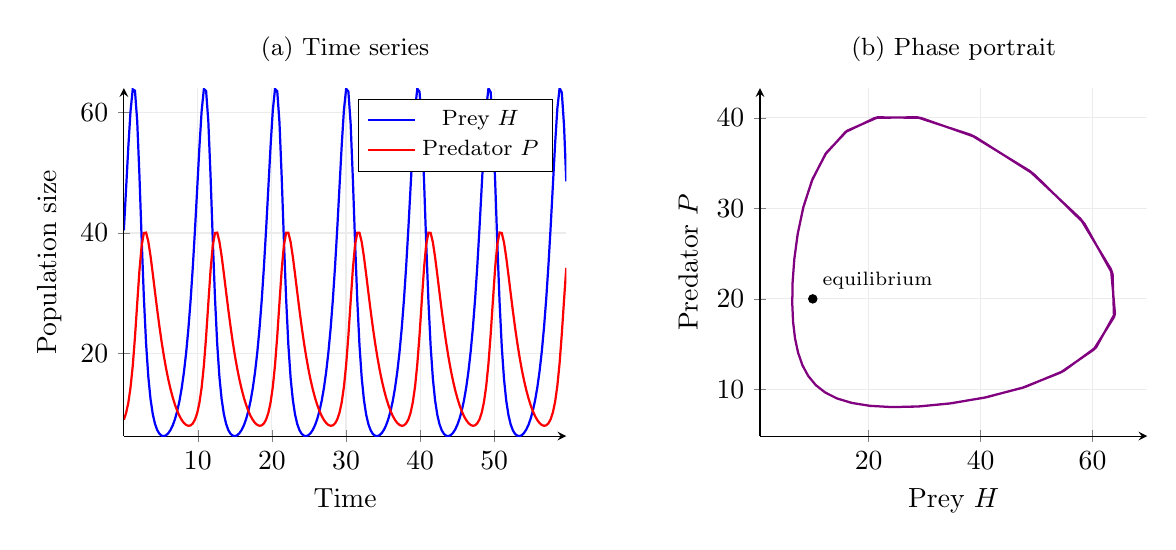
\begin{tikzpicture}
\begin{axis}[
  width=7.2cm, height=6cm,
  xlabel={Time}, ylabel={Population size},
  axis lines=left, enlargelimits=false,
  legend pos=north east, legend style={font=\footnotesize},
  grid=major, grid style={gray!15},
  title={\small (a) Time series},
  name=timeplot
]
\addplot[thick, blue, mark=none] coordinates {(0.02,40.44)(0.32,47.30)(0.62,54.20)(0.92,60.18)(1.22,63.83)(1.52,63.59)(1.82,58.59)(2.12,49.64)(2.42,39.07)(2.72,29.33)(3.02,21.67)(3.32,16.19)(3.62,12.46)(3.92,9.99)(4.22,8.37)(4.52,7.34)(4.82,6.72)(5.12,6.40)(5.42,6.33)(5.72,6.47)(6.02,6.81)(6.32,7.35)(6.62,8.12)(6.92,9.14)(7.22,10.46)(7.52,12.13)(7.82,14.24)(8.12,16.85)(8.42,20.07)(8.72,23.99)(9.02,28.70)(9.32,34.24)(9.62,40.56)(9.92,47.42)(10.22,54.31)(10.52,60.27)(10.82,63.87)(11.12,63.55)(11.42,58.47)(11.72,49.46)(12.02,38.89)(12.32,29.18)(12.62,21.56)(12.92,16.11)(13.22,12.41)(13.52,9.95)(13.82,8.35)(14.12,7.32)(14.42,6.71)(14.72,6.40)(15.02,6.33)(15.32,6.47)(15.62,6.82)(15.92,7.36)(16.22,8.13)(16.52,9.16)(16.82,10.48)(17.12,12.17)(17.42,14.28)(17.72,16.90)(18.02,20.13)(18.32,24.07)(18.62,28.79)(18.92,34.34)(19.22,40.67)(19.52,47.54)(19.82,54.43)(20.12,60.35)(20.42,63.90)(20.72,63.50)(21.02,58.34)(21.32,49.28)(21.62,38.71)(21.92,29.03)(22.22,21.44)(22.52,16.03)(22.82,12.36)(23.12,9.92)(23.42,8.33)(23.72,7.31)(24.02,6.70)(24.32,6.40)(24.62,6.33)(24.92,6.48)(25.22,6.82)(25.52,7.37)(25.82,8.15)(26.12,9.18)(26.42,10.51)(26.72,12.20)(27.02,14.32)(27.32,16.95)(27.62,20.20)(27.92,24.14)(28.22,28.88)(28.52,34.45)(28.82,40.79)(29.12,47.66)(29.42,54.54)(29.72,60.44)(30.02,63.93)(30.32,63.45)(30.62,58.21)(30.92,49.10)(31.22,38.53)(31.52,28.88)(31.82,21.33)(32.12,15.96)(32.42,12.31)(32.72,9.88)(33.02,8.30)(33.32,7.30)(33.62,6.69)(33.92,6.39)(34.22,6.33)(34.52,6.48)(34.82,6.83)(35.12,7.38)(35.42,8.16)(35.72,9.20)(36.02,10.53)(36.32,12.23)(36.62,14.36)(36.92,17.00)(37.22,20.26)(37.52,24.22)(37.82,28.97)(38.12,34.55)(38.42,40.90)(38.72,47.79)(39.02,54.66)(39.32,60.53)(39.62,63.96)(39.92,63.40)(40.22,58.08)(40.52,48.93)(40.82,38.35)(41.12,28.73)(41.42,21.22)(41.72,15.88)(42.02,12.25)(42.32,9.85)(42.62,8.28)(42.92,7.28)(43.22,6.69)(43.52,6.39)(43.82,6.33)(44.12,6.49)(44.42,6.84)(44.72,7.40)(45.02,8.18)(45.32,9.22)(45.62,10.56)(45.92,12.26)(46.22,14.40)(46.52,17.05)(46.82,20.32)(47.12,24.29)(47.42,29.06)(47.72,34.65)(48.02,41.02)(48.32,47.91)(48.62,54.77)(48.92,60.61)(49.22,63.99)(49.52,63.35)(49.82,57.95)(50.12,48.75)(50.42,38.17)(50.72,28.58)(51.02,21.11)(51.32,15.80)(51.62,12.20)(51.92,9.82)(52.22,8.26)(52.52,7.27)(52.82,6.68)(53.12,6.39)(53.42,6.34)(53.72,6.49)(54.02,6.85)(54.32,7.41)(54.62,8.19)(54.92,9.24)(55.22,10.59)(55.52,12.30)(55.82,14.44)(56.12,17.10)(56.42,20.38)(56.72,24.37)(57.02,29.15)(57.32,34.76)(57.62,41.13)(57.92,48.03)(58.22,54.88)(58.52,60.69)(58.82,64.01)(59.12,63.30)(59.42,57.82)(59.72,48.57)};
\addlegendentry{Prey $H$}
\addplot[thick, red, mark=none] coordinates {(0.02,9.05)(0.32,10.14)(0.62,11.83)(0.92,14.37)(1.22,17.97)(1.52,22.72)(1.82,28.28)(2.12,33.72)(2.42,37.88)(2.72,40.00)(3.02,40.07)(3.32,38.60)(3.62,36.18)(3.92,33.29)(4.22,30.26)(4.52,27.30)(4.82,24.50)(5.12,21.93)(5.42,19.61)(5.72,17.54)(6.02,15.71)(6.32,14.11)(6.62,12.72)(6.92,11.52)(7.22,10.52)(7.52,9.69)(7.82,9.02)(8.12,8.52)(8.42,8.19)(8.72,8.04)(9.02,8.10)(9.32,8.42)(9.62,9.07)(9.92,10.16)(10.22,11.87)(10.52,14.42)(10.82,18.04)(11.12,22.81)(11.42,28.37)(11.72,33.81)(12.02,37.94)(12.32,40.01)(12.62,40.06)(12.92,38.56)(13.22,36.13)(13.52,33.24)(13.82,30.21)(14.12,27.25)(14.42,24.46)(14.72,21.89)(15.02,19.57)(15.32,17.51)(15.62,15.68)(15.92,14.08)(16.22,12.69)(16.52,11.51)(16.82,10.50)(17.12,9.67)(17.42,9.01)(17.72,8.51)(18.02,8.19)(18.32,8.04)(18.62,8.11)(18.92,8.43)(19.22,9.08)(19.52,10.19)(19.82,11.91)(20.12,14.47)(20.42,18.11)(20.72,22.90)(21.02,28.47)(21.32,33.89)(21.62,37.99)(21.92,40.03)(22.22,40.04)(22.52,38.53)(22.82,36.08)(23.12,33.19)(23.42,30.16)(23.72,27.20)(24.02,24.41)(24.32,21.85)(24.62,19.54)(24.92,17.47)(25.22,15.65)(25.52,14.05)(25.82,12.67)(26.12,11.49)(26.42,10.49)(26.72,9.66)(27.02,9.00)(27.32,8.51)(27.62,8.18)(27.92,8.04)(28.22,8.11)(28.52,8.44)(28.82,9.10)(29.12,10.21)(29.42,11.94)(29.72,14.53)(30.02,18.19)(30.32,22.99)(30.62,28.57)(30.92,33.98)(31.22,38.04)(31.52,40.05)(31.82,40.03)(32.12,38.49)(32.42,36.03)(32.72,33.13)(33.02,30.11)(33.32,27.15)(33.62,24.36)(33.92,21.81)(34.22,19.50)(34.52,17.44)(34.82,15.62)(35.12,14.03)(35.42,12.65)(35.72,11.47)(36.02,10.47)(36.32,9.65)(36.62,8.99)(36.92,8.50)(37.22,8.18)(37.52,8.04)(37.82,8.11)(38.12,8.45)(38.42,9.11)(38.72,10.23)(39.02,11.98)(39.32,14.58)(39.62,18.26)(39.92,23.08)(40.22,28.67)(40.52,34.06)(40.82,38.10)(41.12,40.06)(41.42,40.01)(41.72,38.46)(42.02,35.99)(42.32,33.08)(42.62,30.06)(42.92,27.10)(43.22,24.32)(43.52,21.77)(43.82,19.46)(44.12,17.41)(44.42,15.59)(44.72,14.00)(45.02,12.63)(45.32,11.45)(45.62,10.45)(45.92,9.63)(46.22,8.98)(46.52,8.49)(46.82,8.17)(47.12,8.04)(47.42,8.12)(47.72,8.46)(48.02,9.13)(48.32,10.26)(48.62,12.02)(48.92,14.63)(49.22,18.33)(49.52,23.17)(49.82,28.77)(50.12,34.15)(50.42,38.15)(50.72,40.08)(51.02,40.00)(51.32,38.42)(51.62,35.94)(51.92,33.03)(52.22,30.00)(52.52,27.05)(52.82,24.27)(53.12,21.72)(53.42,19.42)(53.72,17.37)(54.02,15.56)(54.32,13.98)(54.62,12.61)(54.92,11.43)(55.22,10.44)(55.52,9.62)(55.82,8.97)(56.12,8.49)(56.42,8.17)(56.72,8.04)(57.02,8.12)(57.32,8.46)(57.62,9.14)(57.92,10.28)(58.22,12.05)(58.52,14.69)(58.82,18.41)(59.12,23.27)(59.42,28.87)(59.72,34.23)};
\addlegendentry{Predator $P$}
\end{axis}
\begin{axis}[
  at={(timeplot.right of south east)}, anchor=left of south west, xshift=1.3cm,
  width=6.5cm, height=6cm,
  xlabel={Prey $H$}, ylabel={Predator $P$},
  axis lines=left, enlargelimits=true,
  grid=major, grid style={gray!15},
  title={\small (b) Phase portrait}
]
\addplot[thick, violet, mark=none] coordinates {(40.44,9.05)(47.30,10.14)(54.20,11.83)(60.18,14.37)(63.83,17.97)(63.59,22.72)(58.59,28.28)(49.64,33.72)(39.07,37.88)(29.33,40.00)(21.67,40.07)(16.19,38.60)(12.46,36.18)(9.99,33.29)(8.37,30.26)(7.34,27.30)(6.72,24.50)(6.40,21.93)(6.33,19.61)(6.47,17.54)(6.81,15.71)(7.35,14.11)(8.12,12.72)(9.14,11.52)(10.46,10.52)(12.13,9.69)(14.24,9.02)(16.85,8.52)(20.07,8.19)(23.99,8.04)(28.70,8.10)(34.24,8.42)(40.56,9.07)(47.42,10.16)(54.31,11.87)(60.27,14.42)(63.87,18.04)(63.55,22.81)(58.47,28.37)(49.46,33.81)(38.89,37.94)(29.18,40.01)(21.56,40.06)(16.11,38.56)(12.41,36.13)(9.95,33.24)(8.35,30.21)(7.32,27.25)(6.71,24.46)(6.40,21.89)(6.33,19.57)(6.47,17.51)(6.82,15.68)(7.36,14.08)(8.13,12.69)(9.16,11.51)(10.48,10.50)(12.17,9.67)(14.28,9.01)(16.90,8.51)(20.13,8.19)(24.07,8.04)(28.79,8.11)(34.34,8.43)(40.67,9.08)(47.54,10.19)(54.43,11.91)(60.35,14.47)(63.90,18.11)(63.50,22.90)(58.34,28.47)(49.28,33.89)(38.71,37.99)(29.03,40.03)(21.44,40.04)(16.03,38.53)(12.36,36.08)(9.92,33.19)(8.33,30.16)(7.31,27.20)(6.70,24.41)(6.40,21.85)(6.33,19.54)(6.48,17.47)(6.82,15.65)(7.37,14.05)(8.15,12.67)(9.18,11.49)(10.51,10.49)(12.20,9.66)(14.32,9.00)(16.95,8.51)(20.20,8.18)(24.14,8.04)(28.88,8.11)(34.45,8.44)(40.79,9.10)(47.66,10.21)(54.54,11.94)(60.44,14.53)(63.93,18.19)(63.45,22.99)(58.21,28.57)(49.10,33.98)(38.53,38.04)(28.88,40.05)(21.33,40.03)(15.96,38.49)(12.31,36.03)(9.88,33.13)(8.30,30.11)(7.30,27.15)(6.69,24.36)(6.39,21.81)(6.33,19.50)(6.48,17.44)(6.83,15.62)(7.38,14.03)(8.16,12.65)(9.20,11.47)(10.53,10.47)(12.23,9.65)(14.36,8.99)(17.00,8.50)(20.26,8.18)(24.22,8.04)(28.97,8.11)(34.55,8.45)(40.90,9.11)(47.79,10.23)(54.66,11.98)(60.53,14.58)(63.96,18.26)(63.40,23.08)(58.08,28.67)(48.93,34.06)(38.35,38.10)(28.73,40.06)(21.22,40.01)(15.88,38.46)(12.25,35.99)(9.85,33.08)(8.28,30.06)(7.28,27.10)(6.69,24.32)(6.39,21.77)(6.33,19.46)(6.49,17.41)(6.84,15.59)(7.40,14.00)(8.18,12.63)(9.22,11.45)(10.56,10.45)(12.26,9.63)(14.40,8.98)(17.05,8.49)(20.32,8.17)(24.29,8.04)(29.06,8.12)(34.65,8.46)(41.02,9.13)(47.91,10.26)(54.77,12.02)(60.61,14.63)(63.99,18.33)(63.35,23.17)(57.95,28.77)(48.75,34.15)(38.17,38.15)(28.58,40.08)(21.11,40.00)(15.80,38.42)(12.20,35.94)(9.82,33.03)(8.26,30.00)(7.27,27.05)(6.68,24.27)(6.39,21.72)(6.34,19.42)(6.49,17.37)(6.85,15.56)(7.41,13.98)(8.19,12.61)(9.24,11.43)(10.59,10.44)(12.30,9.62)(14.44,8.97)(17.10,8.49)(20.38,8.17)(24.37,8.04)(29.15,8.12)(34.76,8.46)(41.13,9.14)(48.03,10.28)(54.88,12.05)(60.69,14.69)(64.01,18.41)(63.30,23.27)(57.82,28.87)(48.57,34.23)};
\addplot[only marks, mark=*, mark size=1.5pt, black] coordinates {(10,20)};
\node at (axis cs:10,20) [above right, font=\scriptsize] {equilibrium};
\end{axis}
\end{tikzpicture}

\vspace{1mm}
\footnotesize Real numerical integration (RK4) of $dH/dt = rH - pHP$, $dP/dt = apHP - mP$ ($r{=}1.0, p{=}0.05, a{=}0.4, m{=}0.5$). (a) Prey (blue) peaks first, predator (red) peaks after with a time lag -- prey crash follows predator peak, then predator crash follows prey trough, endlessly. (b) The same trajectory plotted as prey vs.\ predator traces a closed orbit around the interior equilibrium $(H^*,P^*)=(m/(ap),\,r/p)$ -- neutrally stable cycles (the orbit's size depends only on the starting point, not decaying or growing), the classic (unrealistic) signature of the basic unmodified Lotka--Volterra model discussed in the ``3-part paradox.''
\end{figbox}

\begin{exambox}
This is a direct, elegant answer to the Elton-cycle motivating question: the \emph{simplest possible} predator-prey model, containing no external/extrinsic drivers at all, already produces sustained oscillations from intrinsic dynamics alone. This is exactly the kind of ``simple model, surprisingly rich behaviour'' result that recurs across this course (cf.\ logistic/Ricker/Hassell models in the Population Dynamics \& Chaos topic).
\end{exambox}

\subsubsection*{Key assumptions of the basic L--V model}
\begin{itemize}[leftmargin=*]
\item Prey growth is limited \emph{only} by predation -- no other density dependence (no carrying capacity, no resource limitation).
\item The predator is a \textbf{specialist}: it can only persist if this particular prey species is present (no alternative prey, no generalist switching).
\item No change in the environment during the process (constant parameters).
\item Predator and prey encounter one another \textbf{randomly} in a \textbf{homogeneous} environment (well-mixed, no spatial structure).
\end{itemize}
These are all highly unrealistic -- the slides pose this explicitly as a prompt: \emph{how would you make this more realistic?}

\subsubsection*{A more realistic version: density-dependent prey growth}
Adding a carrying capacity $K$ to the prey equation (logistic-style self-limitation) gives:
\begin{align*}
\frac{dH}{dt} &= rH\left(1-\frac{H}{K}\right) - pHP \\
\frac{dP}{dt} &= apHP - mP
\end{align*}
\begin{keybox}[title=Effect of adding density dependence]
This single change to the prey equation \textbf{removes the neutral oscillations} of the basic model: the predator-prey equilibrium becomes a \textbf{stable point} (damped oscillations spiralling into equilibrium, or a directly stable node, depending on parameters) rather than a family of closed neutral cycles -- shown again via a Populus simulation. This is the first of the ``take a break and reflect'' punchlines below.
\end{keybox}

\begin{exambox}[title={``Take a break and reflect'': the three-part paradox}]
The slides deliberately juxtapose three findings to set up a puzzle, which the following experiments are then used to resolve:
\begin{enumerate}[leftmargin=*]
\item \textbf{Real-life data} (Elton's fur-return records) show population cycles.
\item The \textbf{highly unrealistic} basic L--V model \emph{also} shows population cycles.
\item \textbf{More realistic} L--V models (with density-dependent prey growth) \textbf{do not} show sustained cycles -- they damp to a stable equilibrium instead.
\end{enumerate}
So: if realism kills the cycles in the model, what actually sustains cycles in nature? $\to$ the class turns to laboratory experiments for an answer.
\end{exambox}

\subsection{Laboratory tests: Gause's \textit{Paramecium}--\textit{Didinium} experiments}
Gause tested the L--V predictions directly using \textit{Paramecium} (prey) and \textit{Didinium} (predator, a ciliate that consumes \textit{Paramecium}) in simple lab microcosms, under three conditions:
\begin{center}
\begin{tabularx}{\textwidth}{@{}l X@{}}
\toprule
\textbf{Condition} & \textbf{Outcome} \\
\midrule
(a) No refugia (nowhere for prey to hide) & Predator eats all prey, then predator itself goes extinct (both extinct). \\
(b) With refugia (a hiding place for some prey) & Prey partially protected, but the system \emph{still} collapses to extinction (predator starves out of reach of prey, or timing simply delays rather than prevents collapse). \\
(c) With constant immigration (one prey $+$ one predator added externally every third day) & \textbf{Sustained oscillations} were obtained. \\
\bottomrule
\end{tabularx}
\end{center}

\begin{keybox}[title=Gause's conclusion]
Left to itself, the \textit{Paramecium}--\textit{Didinium} system is driven to \textbf{extinction} -- it does \emph{not} self-sustain oscillations. Sustained oscillations were only possible with \textbf{constant interference/input from outside the system} (external immigration), i.e.\ the system needs an external driver to keep cycling, echoing the ``more realistic model $\to$ no cycles'' result above and reinforcing that the basic L--V model's neutral cycles are a mathematical artifact of its unrealistic assumptions, not something real closed populations naturally sustain.
\end{keybox}

\subsection{Huffaker's experiments: adding spatial heterogeneity}
Gause's system was criticized as \textbf{too simple, lacking environmental heterogeneity}. Huffaker tested two mite species -- \textit{Eotetranychus sexmaculatus} (prey) and \textit{Typhlodromus occidentalis} (predator) -- on arrays of oranges (some whole, some partly covered/isolated) providing a spatially distributed, patchy habitat.

\begin{keybox}[title=Huffaker's key findings]
\begin{itemize}[leftmargin=*]
\item Oscillations could only be obtained with a \textbf{complicated spatial arrangement of patches} (increasing distances between oranges, partial barriers to dispersal, etc.) -- a simple, well-mixed arena (like Gause's) still collapsed to extinction.
\item The \textbf{distribution and relative abundance} of predator and prey mites changed continuously over time and space.
\item \textbf{Prey need some advantage to survive} -- in this system, superior/faster \textbf{dispersal ability} was the prey's advantage, letting it colonize new patches ahead of the predator.
\item \textbf{Metapopulation dynamics} (a shifting mosaic of local extinctions and recolonizations across patches) promote prey survivorship overall, even though any single local (patch-level) prey population is likely to go extinct once the predator arrives there.
\item If the predator is efficient, the prey can persist \emph{only} in a sufficiently \textbf{patchy environment} -- spatial structure, not any single local refuge, is what rescues the system from the Gause-style collapse.
\end{itemize}
\end{keybox}

\begin{exambox}
Read Gause and Huffaker together as a single narrative arc: Gause showed a simple, spatially homogeneous system collapses without external forcing; Huffaker showed that adding \textbf{spatial heterogeneity/patchiness} (not external immigration) can \emph{also} sustain oscillations -- i.e.\ spatial structure is an alternative, more ``natural'' stabilizing mechanism to Gause's artificial constant-immigration trick. This is a recurring theme across the course: intrinsic instability in a simple/well-mixed model can be rescued either by adding realistic self-limitation (which damps oscillations to a stable point, as in the logistic-prey L--V variant) or by adding spatial structure (which can instead \emph{sustain} oscillations/persistence, as here).
\end{exambox}

A general ecological point drawn from this section: predators can substantially reduce prey population size in nature, and are \textbf{sometimes more effective than pesticides} at doing so (a segue toward the economic/biological-control relevance of predation raised at the start of the topic).

\subsection{What's actually happening in nature?}
The slides are candid that real predator-prey dynamics in nature are \textbf{very complicated}, with ``all kinds of dynamics'' observed empirically (stable equilibria, damped oscillations, sustained cycles, chaos, extinctions) rather than one clean universal pattern. Possible reasons given for this complexity:
\begin{itemize}[leftmargin=*]
\item Multiple-prey, multiple-predator systems (not the simple 1-predator/1-prey L--V setup).
\item Spatial heterogeneity, including refugia (cf.\ Huffaker).
\item Predator efficiency changing across time (e.g.\ with predator learning, prey density, or environmental conditions).
\item Evolutionary changes in both prey and predator (ongoing coevolutionary arms races -- a direct segue into the anti-predator adaptations covered next).
\end{itemize}

\subsection{Prey strategies for predator avoidance}
The second half of the topic shifts from population-level dynamics to individual/evolutionary anti-predator adaptations, organized into three categories: coloration, behavioural, and chemical.

\subsubsection*{Coloration strategies}
\begin{center}
\begin{tabularx}{\textwidth}{@{}l X@{}}
\toprule
\textbf{Strategy} & \textbf{Definition \& example} \\
\midrule
\textbf{Aposematic (warning) coloration} & Markings that make a dangerous, poisonous, or foul-tasting animal particularly \emph{conspicuous} and recognizable to a predator -- advertising unprofitability rather than hiding it. Slide example: \textit{Sympetrum flaveolum} (yellow-winged darter dragonfly). \\
\textbf{Crypsis} & Camouflage -- blending in with the background/environment to avoid detection altogether. Slide examples: dead-leaf mantis, tawny frogmouth (bark-mimicking bird), leaf-mimicking mantis (\textit{Choeradodis rhomboidea}), lantern fly. \\
\bottomrule
\end{tabularx}
\end{center}

\begin{keybox}[title=Mimicry -- two types (key exam distinction)]
\textbf{Mimicry} = attempts by one species to resemble another species (or a feature of the environment) so as to gain an anti-predation benefit. Two broad types, distinguished by whether the mimic actually \emph{has} the defence it signals:
\begin{itemize}[leftmargin=*]
\item \textbf{Batesian mimicry}: the mimic sends signals \emph{similar to} a genuinely defended model species, but does \textbf{not} itself share the attribute that makes the model unprofitable to predators (e.g.\ it is not actually unpalatable/toxic) -- it is essentially ``bluffing.'' Example: drone fly mimicking a honey bee (harmless fly resembling a stinging bee).
\item \textbf{M\"ullerian mimicry}: two (or more) species share very similar warning signals \emph{and} both \textbf{genuinely} possess an anti-predation attribute (e.g.\ both are unpalatable). Because a shared predator that learns to avoid the signal from an encounter with \emph{either} species then avoids both, individuals of \emph{both} species benefit -- mutual reinforcement rather than one species exploiting the other. Example: \textit{Heliconius} butterflies.
\end{itemize}
The key discriminator to remember for exams: Batesian = one honest signaller $+$ one dishonest free-rider; M\"ullerian = multiple honest signallers converging on a shared warning signal for mutual benefit.
\end{keybox}

\subsubsection*{Behavioural strategies}
\begin{center}
\begin{tabularx}{\textwidth}{@{}l X@{}}
\toprule
\textbf{Strategy} & \textbf{Definition \& example} \\
\midrule
\textbf{Catalepsis} & Playing dead so the predator loses interest/ignores the prey (many predators are triggered primarily by movement). Example: opossums (\textit{Didelphis virginiana}); also demonstrated in Costa Rican katydids. \\
\textbf{Intimidation display} & An attempt to startle the predator long enough to escape, or to convince the predator the prey would be too costly to attack (e.g.\ sudden eyespot flashing in moths). \\
\textbf{Group living} & Helps via increased collective watchfulness (more eyes/ears to detect predators), \textbf{mobbing} (group harassment of a predator to drive it off, seen in birds), and predator confusion (harder to target one individual in a moving group); also enables \textbf{alarm calls} and \textbf{alarm pheromones} (e.g.\ in aphids) to warn groupmates. \\
\bottomrule
\end{tabularx}
\end{center}

\subsubsection*{Chemical strategies}
Making the prey \textbf{too toxic, too smelly, or too distasteful} to be worth eating. Slide examples: badgers and skunks (noxious spray), bombardier beetle (\textit{Bradinus crepitans}, sprays a hot, irritating chemical defence).

\begin{exambox}
Important caveat stated explicitly on the slides: \textbf{toxins can poison the predator, but this alone often does not save the individual prey} that has already been attacked/consumed -- the toxin punishes the predator \emph{after the fact} and thereby trains it to avoid the prey type in future, but doesn't necessarily save that particular individual. For a chemical defence to be maximally effective as a \emph{deterrent} (rather than only a delayed-selection mechanism), it generally needs to be paired with \textbf{aposematic (warning) coloration} so the predator can learn to recognize and avoid the signal \emph{before} attacking -- directly linking the chemical and coloration strategy categories.
\end{exambox}

\begin{keybox}[title=Topic summary]
Predation was covered at two levels: (i) \textbf{population dynamics} -- the basic L--V model gives neutral intrinsic oscillations, but this is fragile (realistic self-limitation kills the cycles; simple lab systems collapse to extinction without either external forcing (Gause) or spatial heterogeneity (Huffaker)) -- so real-world cycles (e.g.\ Elton's fur data) likely reflect some combination of multi-species interactions, spatial structure, time-varying predator efficiency, and coevolution, not the bare two-species L--V mechanism alone; and (ii) \textbf{anti-predator adaptation} -- coloration (aposematism, crypsis, Batesian vs.\ M\"ullerian mimicry), behaviour (catalepsis, intimidation, group living), and chemical defence, several of which interact (e.g.\ toxin $+$ aposematism).
\end{keybox}

\newpage

% =====================================================================
\section{Eutrophication: Trophic Classification, Alternative Stable States, and Lake Restoration}

\subsection{Classical and modern views of lake trophic status}
\textbf{Classical view (Naumann \& Thienemann):} lakes were classified into discrete types based on productivity and water character:
\begin{center}
\begin{tabularx}{\textwidth}{@{}l X@{}}
\toprule
\textbf{Type} & \textbf{Character} \\
\midrule
Oligotrophy & Little productivity, clear water. \\
Eutrophy & High productivity, greenish water due to phytoplankton. \\
Dystrophy & Low conductivity, water colored brown by dissolved humic substances. \\
Extinction & (The lake's terminal/senescent state -- filled in, no longer a lake.) \\
\bottomrule
\end{tabularx}
\end{center}

\begin{keybox}[title={Modern view: a continuum, not discrete boxes}]
``Oligotrophic'' and ``eutrophic'' are now understood as regions of a \textbf{trophic continuum}, separated only by operationally established limits -- e.g.\ total phosphorus concentration ($P_{\text{tot}}$) measured during spring circulation (the seasonal mixing event when the water column overturns). Since trophic condition is fundamentally a \emph{biological} phenomenon (not just a chemistry number), several criteria (nutrient levels, algal biomass, water clarity, species composition) need to be considered together to describe it properly, not $P_{\text{tot}}$ alone. (Source: Lampert \& Sommer, \textit{Limnoecology}.)
\end{keybox}

\subsection{What determines a lake's trophic status?}
\begin{center}
\begin{tabularx}{\textwidth}{@{}l X@{}}
\toprule
\textbf{Factor} & \textbf{Details} \\
\midrule
1. Original basin shape & Mean depth of the basin. \\
2. Nature of the drainage basin & Erosion rates; soil composition $\to$ determines nutrient inputs from the catchment. \\
3. Climate & Rain and snowfall; mean temperature. \\
4. Human activity (\textbf{cultural eutrophication}) & Fertilizers; human waste products (domestic, industrial). \\
\bottomrule
\end{tabularx}
\end{center}

\subsection{The mechanism: how a lake goes from oligotrophic to eutrophic}
\begin{enumerate}[leftmargin=1.5em]
\item \textbf{Nutrient enrichment}, particularly of \textbf{phosphorus} -- from natural sources, or anthropogenic ones (urban, industrial, agricultural runoff).
\item \textbf{Increased organic matter production} (eutrophication proper): increased algal blooms, often dominated by blue-green algae/cyanobacteria (e.g.\ \textit{Anabaena}, \textit{Microcystis}); this reduces light availability to submerged plants, and reduces dissolved oxygen -- particularly in the \textbf{hypolimnion} (the cold, stagnant bottom layer of a stratified lake, cut off from atmospheric re-oxygenation). Low-oxygen conditions there trigger a series of \textbf{anoxic (reducing) chemical reactions that release phosphorus} back from the sediment into the water column (internal P loading) and \textbf{increase the pH} of the water.
\item \textbf{Death of fish and other aquatic life} (fish-kill), as oxygen is depleted and toxic byproducts accumulate.
\end{enumerate}

\begin{exambox}
Note the \textbf{positive feedback loop} embedded in step 2: hypoxia in the hypolimnion releases \emph{more} phosphorus from the sediment, which fuels \emph{more} algal growth, which further depletes oxygen -- eutrophication is self-reinforcing once it gets going, not a simple one-shot response to nutrient input. Also note: this is emphatically \textbf{not a problem confined to small lakes} -- the slides cite the large-scale eutrophication-linked fish-kill events in the Caspian Sea (2003) as a reminder of scale.
\end{exambox}

\subsection{The classic recovery story: Lake Washington, Seattle}
\begin{keybox}[title=Timeline]
\begin{itemize}[leftmargin=*]
\item \textbf{1940s}: Lake Washington was oligotrophic.
\item \textbf{1950s--60s}: Sewage was discharged directly into the lake $\to$ oligotrophic state collapsed into a foul, algae-choked state nicknamed \textbf{``Lake Stinko.''}
\item Research by \textbf{W.T. Edmondson (1970)} implicated sewage-borne phosphorus as the cause.
\item Sewage was diverted away from the lake (to Puget Sound instead).
\item With reduced phosphorus levels, the lake's condition improved; \textbf{further} improvement followed when \textbf{\textit{Daphnia}} (a phytoplankton-grazing zooplankton) recovered once the cyanobacteria that had been fouling its feeding apparatus disappeared.
\item Over time, detergent manufacturers also reduced phosphate levels in their products, reducing a major ongoing P source.
\end{itemize}
\end{keybox}

\begin{papbox}[title={Paper Summary: ``Rescue of Lake Stinko'' -- the story of the Lake Washington restoration (University of Washington, based on W.T.\ Edmondson's research)}]
\textbf{What kind of source this is:} a narrative science-history account (not a primary research paper), but listed on the course's own reading list as a ``Paper''-tier item, so it is summarized here for the fuller detail it adds beyond the slide bullet points above.

\textbf{The story, in more detail:} In 1955, a researcher in Edmondson's lab noticed Lake Washington's water had turned cloudy; lab analysis found \textit{Oscillatoria rubescens}, a cyanobacterium recognized (from prior experience with European lakes) as a classic tell-tale early-warning sign of lake deterioration. Seattle had been discharging raw sewage into the lake since $\sim$1900; by 1941 the city's own sewage was diverted away, but \textbf{suburban} sewage treatment plants proliferated around the lake through the 1940s--50s (ten plants by 1953, jointly discharging $\sim$80 million litres/day), reintroducing the same phosphorus-loading problem from a different, more diffuse source.

Edmondson's key public-communication move was preparing a clear, jargon-free, question-and-answer style report for the chair of Seattle's Metropolitan Problems Advisory Committee, laying out a phosphorus-vs-algae ``budget'' in terms policymakers could act on. This informed the creation of \textbf{``Metro,'' a new metropolitan government body} (approved by referendum in 1958) tasked with diverting sewage away from the lake via a major trunk sewer to Puget Sound.

\textbf{Key conclusions/lessons:}
\begin{itemize}[leftmargin=1.3em,nosep]
\item There was a \textbf{multi-year lag} between the political decision (1958) and the infrastructure actually being operational ($\sim$1963), during which the lake's condition continued to worsen exactly as Edmondson had predicted (giving rise to the ``Lake Stinko'' nickname in the press) -- a caution that ecological remediation often has a long, painful lag before results show.
\item Recovery, once effluent diversion took hold ($\sim$1964 onward), was \textbf{faster and more complete than even Edmondson had predicted}: by 1971 the lake was clearer than in 1950, and it is now roughly twice as clear as in 1950.
\item The extra improvement beyond what phosphorus reduction alone would predict is attributed to a \textbf{trophic cascade}: as pollutant-tolerant \textit{Oscillatoria} declined, it stopped fouling \textit{Daphnia}'s feeding apparatus, so \textit{Daphnia} numbers rebounded from around 1976 and their grazing further suppressed algae -- i.e.\ the biological recovery mechanism (Daphnia grazing pressure) compounded the chemical one (reduced P input).
\item Edmondson's own reflection, worth remembering as a general point about the science-policy relationship: his original research was pursued as pure \textbf{basic research} into lake productivity/community structure with no explicit pollution-control mandate, yet it turned out to supply exactly the predictive understanding that the practical clean-up effort needed -- \emph{``applied research cannot be done effectively without a background of information developed by basic research.''}
\end{itemize}
\end{papbox}

A more modern parallel case flagged on the slides (not covered in the same depth): \textbf{Lake Erie}, where nutrient loading and eutrophication remain an active, ongoing management problem.

\subsection{Why isn't ``just reduce phosphate'' enough? Alternative stable states}
The naive expectation -- eutrophication is caused by excess phosphate, so simply reducing phosphate input should reverse it -- turns out to be \textbf{not so simple}, as demonstrated dramatically by many real restoration attempts that failed to produce recovery even after substantial nutrient reduction. The slides use \textbf{Scheffer et al.\ (2001, \textit{Nature})} to explain why.

\begin{papbox}[title={Paper Summary: Scheffer, Carpenter, Foley, Folke \& Walker (2001), \textit{Nature} 413:591--596 -- ``Catastrophic Shifts in Ecosystems''}]
\textbf{Scope:} A synthesis/review paper arguing that many ecosystems -- lakes, coral reefs, oceans, forests, arid lands -- do \emph{not} respond smoothly and reversibly to gradual environmental change, but can instead undergo sudden, drastic switches between \textbf{alternative stable states}, and that understanding \emph{resilience} (not just the current state) is key to managing this.

\textbf{The core theoretical framework:}
\begin{itemize}[leftmargin=1.3em,nosep]
\item If an ecosystem's equilibrium response curve, plotted against a slowly changing external condition, is ``folded back'' on itself, the system has \textbf{two alternative stable states for the same external conditions}, separated by an unstable equilibrium (the boundary between their ``basins of attraction'').
\item Once on the upper branch, gradually worsening conditions produce \emph{little visible change} until a critical threshold (a \textbf{fold/saddle-node bifurcation}, labelled $F_2$) is crossed, at which point a sudden, ``catastrophic'' jump to the lower branch occurs -- often catching managers by surprise because there was no gradual warning.
\item Critically, simply reversing the external condition back to its pre-collapse level is \textbf{not enough} to flip the system back -- one must push conditions back further, past a \emph{different} threshold $F_1$, before the system snaps back up to the upper branch. This asymmetry between the forward and backward switching points is called \textbf{hysteresis}.
\item \textbf{Resilience} is defined (following Holling 1973) as the size of a state's ``basin of attraction'' -- how large a perturbation the system can absorb without being tipped into the alternative state. Gradual environmental change can silently \textbf{shrink resilience} (make the basin smaller) long before the state itself visibly changes, making the system increasingly fragile to ordinary stochastic disturbances even while it still looks fine.
\end{itemize}

\begin{keybox}[title={The minimal ``Box 1'' mathematical model (lakes/desertification)}]
A simple model showing hysteresis takes the general form of a rate of increase (nutrient recycling, in the lake interpretation) that is an accelerating (Hill-function-shaped) function of the state variable $x$, competing against a constant linear decay/loss term. Steeper (more switch-like) Hill functions produce \textbf{stronger hysteresis}. Interpreted for eutrophication, $x$ = internal nutrient recycling/phytoplankton biomass; interpreted for desertification, $x$ = barren land, with the loss term representing erosion by wind/runoff. The same simple mathematical skeleton underlies both phenomena -- the point being that a wide range of superficially unrelated ecosystem collapses share a common mathematical structure.
\end{keybox}

\textbf{Applied to shallow lakes specifically:} the pristine state is clear water with abundant submerged vegetation. Nutrient loading pushes the system toward turbidity, but water clarity is often \textbf{surprisingly unresponsive to nutrient increases up to a threshold}, after which the lake abruptly flips from clear to turbid. Once flipped, \textbf{vegetation itself was suppressing turbidity} via several mechanisms (removing nutrients from the water column, providing refuge for \textit{Daphnia} against fish predation, preventing sediment resuspension) -- so once vegetation is lost, those stabilizing mechanisms disappear too, and the turbid state becomes \emph{self-reinforcing} (fish, now unconstrained by plant refuges, control \textit{Daphnia} and resuspend sediment while foraging, both of which maintain turbidity). This is precisely why reducing nutrients back to pre-collapse levels alone typically fails to restore clarity -- the system needs to be pushed past the (lower) $F_1$ threshold, which is very demanding.

\textbf{Broader context (catastrophe theory):} the paper frames this as one instance of a general phenomenon studied under \textbf{catastrophe theory}, with other cited examples including Sahara desertification, coral reef collapse, and (analogously, outside ecology) poverty traps and stock market crashes. \textbf{Management implication (the paper's central policy message):} because gradual loss of resilience precedes and enables catastrophic shifts, sustainable management should focus on \textbf{maintaining/building resilience} (the size of the safe operating basin), not merely on controlling the current state or preventing individual disturbance events.
\end{papbox}

\begin{figbox}[title={Alternative stable states and hysteresis in shallow lakes (Scheffer et al.\ 2001)}]
\centering
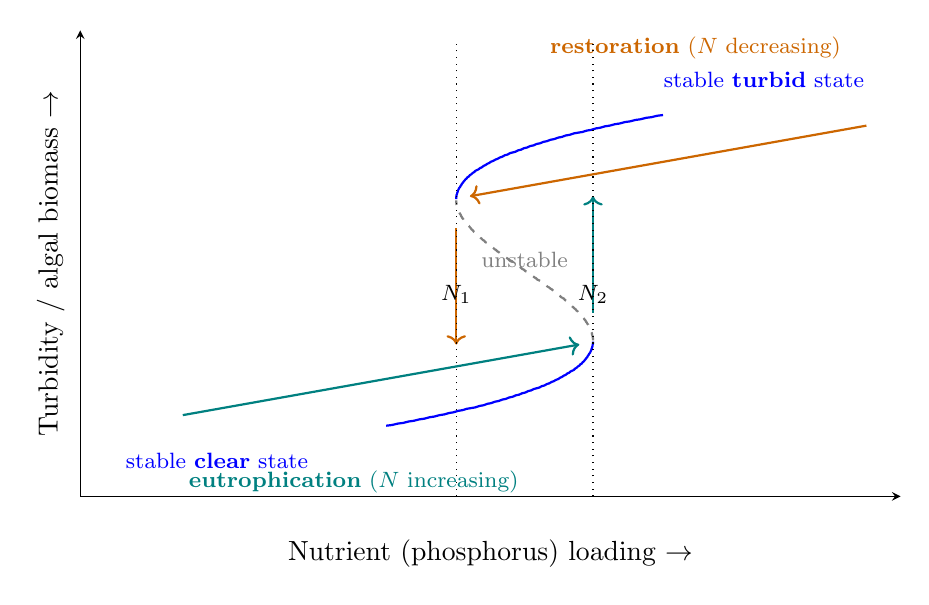
\begin{tikzpicture}
\begin{axis}[
  width=12cm, height=7.5cm,
  xlabel={Nutrient (phosphorus) loading $\to$}, ylabel={Turbidity / algal biomass $\to$}, xlabel style={yshift=-10pt},
  xmin=-8, xmax=16, ymin=-3.2, ymax=3.4,
  axis lines=left, enlargelimits=false,
  xtick=\empty, ytick=\empty,
  grid=none, clip=false
]
\addplot[thick, blue, mark=none] coordinates {(0.95,-2.20)(1.12,-2.19)(1.29,-2.17)(1.45,-2.16)(1.61,-2.14)(1.76,-2.13)(1.92,-2.11)(2.07,-2.10)(2.22,-2.08)(2.36,-2.07)(2.51,-2.05)(2.65,-2.04)(2.79,-2.02)(2.92,-2.01)(3.05,-1.99)(3.18,-1.98)(3.31,-1.96)(3.44,-1.95)(3.56,-1.94)(3.68,-1.92)(3.80,-1.91)(3.91,-1.89)(4.02,-1.88)(4.13,-1.86)(4.24,-1.85)(4.35,-1.83)(4.45,-1.82)(4.55,-1.80)(4.65,-1.79)(4.74,-1.77)(4.84,-1.76)(4.93,-1.74)(5.02,-1.73)(5.10,-1.71)(5.19,-1.70)(5.27,-1.68)(5.35,-1.67)(5.43,-1.66)(5.50,-1.64)(5.58,-1.63)(5.65,-1.61)(5.72,-1.60)(5.79,-1.58)(5.85,-1.57)(5.92,-1.55)(5.98,-1.54)(6.04,-1.52)(6.09,-1.51)(6.15,-1.49)(6.20,-1.48)(6.25,-1.46)(6.30,-1.45)(6.35,-1.43)(6.40,-1.42)(6.44,-1.41)(6.48,-1.39)(6.52,-1.38)(6.56,-1.36)(6.60,-1.35)(6.63,-1.33)(6.67,-1.32)(6.70,-1.30)(6.73,-1.29)(6.76,-1.27)(6.78,-1.26)(6.81,-1.24)(6.83,-1.23)(6.85,-1.21)(6.87,-1.20)(6.89,-1.18)(6.91,-1.17)(6.92,-1.16)(6.94,-1.14)(6.95,-1.13)(6.96,-1.11)(6.97,-1.10)(6.98,-1.08)(6.99,-1.07)(6.99,-1.05)(7.00,-1.04)(7.00,-1.02)(7.00,-1.01)};
\addplot[thick, blue, mark=none] coordinates {(3.00,1.01)(3.00,1.02)(3.00,1.04)(3.01,1.05)(3.01,1.07)(3.02,1.08)(3.03,1.10)(3.04,1.11)(3.05,1.13)(3.06,1.14)(3.08,1.16)(3.09,1.17)(3.11,1.18)(3.13,1.20)(3.15,1.21)(3.17,1.23)(3.19,1.24)(3.22,1.26)(3.24,1.27)(3.27,1.29)(3.30,1.30)(3.33,1.32)(3.37,1.33)(3.40,1.35)(3.44,1.36)(3.48,1.38)(3.52,1.39)(3.56,1.41)(3.60,1.42)(3.65,1.43)(3.70,1.45)(3.75,1.46)(3.80,1.48)(3.85,1.49)(3.91,1.51)(3.96,1.52)(4.02,1.54)(4.08,1.55)(4.15,1.57)(4.21,1.58)(4.28,1.60)(4.35,1.61)(4.42,1.63)(4.50,1.64)(4.57,1.66)(4.65,1.67)(4.73,1.68)(4.81,1.70)(4.90,1.71)(4.98,1.73)(5.07,1.74)(5.16,1.76)(5.26,1.77)(5.35,1.79)(5.45,1.80)(5.55,1.82)(5.65,1.83)(5.76,1.85)(5.87,1.86)(5.98,1.88)(6.09,1.89)(6.20,1.91)(6.32,1.92)(6.44,1.94)(6.56,1.95)(6.69,1.96)(6.82,1.98)(6.95,1.99)(7.08,2.01)(7.21,2.02)(7.35,2.04)(7.49,2.05)(7.64,2.07)(7.78,2.08)(7.93,2.10)(8.08,2.11)(8.24,2.13)(8.39,2.14)(8.55,2.16)(8.71,2.17)(8.88,2.19)(9.05,2.20)};
\addplot[thick, dashed, gray, mark=none] coordinates {(7.00,-0.99)(7.00,-0.98)(7.00,-0.96)(6.99,-0.95)(6.99,-0.93)(6.98,-0.92)(6.97,-0.91)(6.97,-0.89)(6.96,-0.88)(6.94,-0.86)(6.93,-0.85)(6.92,-0.83)(6.91,-0.82)(6.89,-0.80)(6.87,-0.79)(6.86,-0.77)(6.84,-0.76)(6.82,-0.74)(6.80,-0.73)(6.78,-0.71)(6.76,-0.70)(6.73,-0.68)(6.71,-0.67)(6.68,-0.65)(6.66,-0.64)(6.63,-0.63)(6.60,-0.61)(6.58,-0.60)(6.55,-0.58)(6.52,-0.57)(6.49,-0.55)(6.46,-0.54)(6.42,-0.52)(6.39,-0.51)(6.36,-0.49)(6.33,-0.48)(6.29,-0.46)(6.26,-0.45)(6.22,-0.43)(6.18,-0.42)(6.15,-0.40)(6.11,-0.39)(6.07,-0.38)(6.03,-0.36)(6.00,-0.35)(5.96,-0.33)(5.92,-0.32)(5.88,-0.30)(5.84,-0.29)(5.80,-0.27)(5.76,-0.26)(5.71,-0.24)(5.67,-0.23)(5.63,-0.21)(5.59,-0.20)(5.55,-0.18)(5.50,-0.17)(5.46,-0.15)(5.42,-0.14)(5.37,-0.13)(5.33,-0.11)(5.29,-0.10)(5.24,-0.08)(5.20,-0.07)(5.15,-0.05)(5.11,-0.04)(5.07,-0.02)(5.02,-0.01)(4.98,0.01)(4.93,0.02)(4.89,0.04)(4.85,0.05)(4.80,0.07)(4.76,0.08)(4.71,0.10)(4.67,0.11)(4.63,0.13)(4.58,0.14)(4.54,0.15)(4.50,0.17)(4.45,0.18)(4.41,0.20)(4.37,0.21)(4.33,0.23)(4.29,0.24)(4.24,0.26)(4.20,0.27)(4.16,0.29)(4.12,0.30)(4.08,0.32)(4.04,0.33)(4.00,0.35)(3.97,0.36)(3.93,0.38)(3.89,0.39)(3.85,0.40)(3.82,0.42)(3.78,0.43)(3.74,0.45)(3.71,0.46)(3.67,0.48)(3.64,0.49)(3.61,0.51)(3.58,0.52)(3.54,0.54)(3.51,0.55)(3.48,0.57)(3.45,0.58)(3.42,0.60)(3.40,0.61)(3.37,0.63)(3.34,0.64)(3.32,0.65)(3.29,0.67)(3.27,0.68)(3.24,0.70)(3.22,0.71)(3.20,0.73)(3.18,0.74)(3.16,0.76)(3.14,0.77)(3.13,0.79)(3.11,0.80)(3.09,0.82)(3.08,0.83)(3.07,0.85)(3.06,0.86)(3.04,0.88)(3.03,0.89)(3.03,0.91)(3.02,0.92)(3.01,0.93)(3.01,0.95)(3.00,0.96)(3.00,0.98)(3.00,0.99)};
\node[blue] at (axis cs:-4,-2.7) {\footnotesize stable \textbf{clear} state};
\node[blue] at (axis cs:12,2.7) {\footnotesize stable \textbf{turbid} state};
\node[gray] at (axis cs:5,0.15) {\footnotesize unstable};
\draw[->, thick, teal] (axis cs:-5,-2.05) -- (axis cs:6.6,-1.05);
\draw[->, thick, teal] (axis cs:7,-0.6) -- (axis cs:7,1.05);
\node[teal] at (axis cs:0,-3.0) {\footnotesize \textbf{eutrophication} ($N$ increasing)};
\draw[->, thick, orange!80!black] (axis cs:15,2.05) -- (axis cs:3.4,1.05);
\draw[->, thick, orange!80!black] (axis cs:3,0.6) -- (axis cs:3,-1.05);
\node[orange!80!black] at (axis cs:10,3.15) {\footnotesize \textbf{restoration} ($N$ decreasing)};
\draw[dotted] (axis cs:3,-3.2) -- (axis cs:3,3.2);
\draw[dotted] (axis cs:7,-3.2) -- (axis cs:7,3.2);
\node at (axis cs:3,0) [below=2pt, font=\footnotesize] {$N_1$};
\node at (axis cs:7,0) [below=2pt, font=\footnotesize] {$N_2$};
\end{axis}
\end{tikzpicture}

\vspace{1mm}
\footnotesize Both the clear-water branch (bottom) and the turbid branch (top) are locally \textbf{stable}; the dashed middle branch is \textbf{unstable} (any small perturbation pushes the lake away from it, toward one of the two stable branches -- it marks the boundary between the two states' basins of attraction). Crucially the two branches don't switch at the same nutrient level: increasing nutrients (teal path) keeps the lake clear until it is pushed all the way past the \emph{upper} fold point $N_2$, where it jumps abruptly to turbid; but once turbid, merely restoring nutrients back below $N_2$ is \textbf{not enough} to reverse it -- nutrients must be cut all the way past the \emph{lower} fold point $N_1$ (orange path) before the lake snaps back to clear. This gap between $N_1$ and $N_2$ is the \textbf{hysteresis}: the system's history (which branch it's currently on), not just its current nutrient level, determines its state whenever $N_1 < N < N_2$. This is exactly why simple nutrient reduction back to ``pre-eutrophication'' levels often fails to restore a lake, and why biomanipulation (direct intervention, e.g.\ fish removal) is frequently needed to force the jump back down.
\end{figbox}

\begin{keybox}[title={Diagram: the shallow-lake interaction web (Scheffer, 1998)}]
The slides give a signed causal-loop diagram (after Scheffer, 1998) linking the state variables of a shallow lake, each arrow marked \textbf{+} (same-direction effect) or \textbf{--} (opposite-direction effect). The instructor's own rule for reading it: \textbf{multiply the signs along a chain of arrows} to get the net effect of the first variable on the last.
\begin{itemize}[leftmargin=1.3em,nosep]
\item \textbf{The core antagonism:} Turbidity $\xrightarrow{-}$ Vegetation and (via Algae) Vegetation $\xrightarrow{-}$ Nutrients $\xrightarrow{+}$ Algae $\xrightarrow{+}$ Turbidity -- so vegetation and turbidity suppress each other both directly and via the nutrient-algae route, which is exactly the mutual antagonism that generates \textbf{two} alternative stable states (vegetation-dominated/clear vs.\ algae-dominated/turbid) rather than one smooth intermediate.
\item \textbf{Vegetation also protects clarity by several independent routes}: it depletes Nutrients ($-$) that would otherwise feed Algae; it produces allelopathic substances ($+$) that suppress Algae ($-$, net effect of vegetation on algae via this route is positive $\times$ negative $=$ negative, i.e.\ vegetation lowers algae); and it dampens Waves ($-$), which lowers Resuspended Sediment ($+$) and hence Turbidity ($+$) -- another route by which more vegetation means less turbidity.
\item \textbf{Fish sit at the root of the destabilizing side:} Fish $\xrightarrow{+}$ Resuspended Sed.\ $\xrightarrow{+}$ Turbidity (net positive -- more fish, more turbidity, directly); and separately Fish $\xrightarrow{-}$ Zooplankton $\xrightarrow{-}$ Algae (two negatives multiply to a net \emph{positive} effect of fish on algae) -- i.e.\ fish promote turbidity/algae growth by two independent routes (physical disturbance, and suppressing the \textit{Daphnia} grazers that would otherwise keep algae down). This is precisely the mechanistic justification for \textbf{biomanipulation}: removing fish cuts both of these positive chains at their root.
\end{itemize}
This is the same qualitative story as the papbox above, but the diagram makes the individual \textbf{mechanistic pathways} explicit -- useful for a question asking you to trace ``how does removing fish affect turbidity'' step by step rather than just naming the two end states.
\end{keybox}

\begin{figbox}[title={Causal loop diagram: the internal-loading feedback in eutrophication}]
\centering
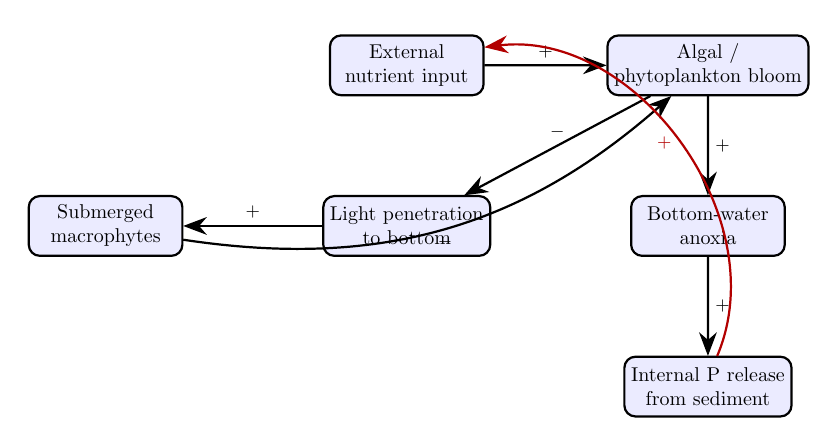
\begin{tikzpicture}[scale=0.85, every node/.style={scale=0.85}, transform shape,
  box/.style={draw, thick, rounded corners, fill=blue!8, align=center, minimum width=2.7cm, minimum height=1.05cm},
  >={Stealth[length=3mm]}
]
\node[box] (nutrients) at (0,4.2) {External\\nutrient input};
\node[box] (algae) at (4.5,4.2) {Algal /\\phytoplankton bloom};
\node[box] (macro) at (-4.5,1.8) {Submerged\\macrophytes};
\node[box] (light) at (0,1.8) {Light penetration\\to bottom};
\node[box] (anoxia) at (4.5,1.8) {Bottom-water\\anoxia};
\node[box] (release) at (4.5,-0.6) {Internal P release\\from sediment};

\draw[->, thick] (nutrients) -- (algae) node[midway, above]{\small $+$};
\draw[->, thick] (algae) -- (light) node[midway, above]{\small $-$};
\draw[->, thick] (light) -- (macro) node[midway, above]{\small $+$};
\draw[->, thick] (macro) to[bend right=25] node[midway, below]{\small $-$} (algae);
\draw[->, thick] (algae) -- (anoxia) node[midway, right]{\small $+$};
\draw[->, thick] (anoxia) -- (release) node[midway, right]{\small $+$};
\draw[->, thick, red!70!black] (release) to[bend right=60] node[midway, left]{\small $+$} (nutrients);
\end{tikzpicture}

\vspace{1mm}
\footnotesize Two nested feedback loops. \textbf{Balancing (self-limiting) loop}: algae $\to$ reduced light $\to$ fewer macrophytes, but macrophytes themselves suppress algae (via nutrient competition, refuge for zooplankton grazers, etc.) -- so losing macrophytes \emph{removes a brake} on algal growth. \textbf{Reinforcing (vicious-cycle) loop} in red: algal blooms $\to$ bottom anoxia (decomposition consumes oxygen) $\to$ anoxic sediments release previously bound phosphorus back into the water column $\to$ \emph{more} nutrients available $\to$ more algae. This second loop is exactly the ``internal loading'' mechanism that explains why cutting external nutrient inputs alone often fails to restore a eutrophic lake quickly: the sediment itself has become an internal nutrient source, sustaining the turbid state independently of external inputs (the mechanistic underpinning of the hysteresis in the figure above).
\end{figbox}

\begin{exambox}
\textbf{Likely conceptual question:} ``Why did reducing phosphorus loading fail to restore lake clarity in many shallow-lake restoration attempts, and what does this imply for management?'' Expected answer: alternative stable states with hysteresis mean the nutrient level required to \emph{cause} the turbid-state collapse is higher than the (much lower) nutrient level required to \emph{reverse} it back to clear -- so restoring pre-collapse nutrient levels lands you in the middle of the hysteresis loop, still within the turbid state's basin of attraction. Effective restoration must either push nutrients further down than the original collapse threshold, or directly intervene in the state variable itself (e.g.\ removing fish/adding vegetation) to help the system escape the turbid basin -- which is exactly the logic behind biomanipulation, below.
\end{exambox}

\subsection{Reversing the trophic state: biomanipulation}
Given that nutrient reduction alone is often insufficient, the slides pose the direct question: \textbf{how do you reverse the trophic state of a shallow lake?} One answer, following directly from the mechanism above (fish suppress \textit{Daphnia}, which otherwise grazes down phytoplankton and helps clear the water): \textbf{reduce the number of fish.}

\begin{keybox}[title={Biomanipulation: Meijer et al.\ (1999)}]
A study of \textbf{18 lakes of varying shape and size in the Netherlands}, monitored over a \textbf{ten-year period} following biomanipulation (fish removal, sometimes combined with predatory-fish stocking). \textbf{Water transparency increased} following biomanipulation across these lakes -- empirical confirmation that directly intervening on the fish/\textit{Daphnia}/turbidity feedback loop (rather than nutrients alone) can help nudge a lake out of the turbid-state basin of attraction, consistent with the alternative-stable-states framework above.
\end{keybox}

\subsection{Scale of the global phosphorus pollution problem}
Per a \textbf{2018 review} (Mekonnen \& Hoekstra, \textit{Water Resources Research}) cited on the slides: globally, human activities dump roughly \textbf{1.5 teragrams} (1.5 billion kg) of phosphorus into freshwater systems \textbf{per year}. By country share of global anthropogenic phosphorus pollution: \textbf{China contributes the most (30\%)}, followed by \textbf{India (8\%)}, the \textbf{USA (7\%)}, and \textbf{Spain and Brazil (6\% each)}. In many regions, either there is not enough water to dilute/assimilate this phosphorus load, or the pollution load is simply too large for the water system to handle -- motivating active restoration methods.

\subsection{Restoration methods (Mandatory reading: S\o{}ndergaard et al.\ 2012)}
S\o{}ndergaard, Jeppesen \& Jensen (2012, \textit{Lake Restoration}, in \textit{Encyclopedia of Lakes and Reservoirs}, pp.\ 455--458) is explicitly listed as \textbf{Mandatory} reading on the slides (unusually, since it is an encyclopedia-chapter source rather than a primary paper -- but the instructor's own classification makes it fully examinable, and its content is directly reproduced as tables on the slides). Restoration methods are grouped into three categories:

\begin{center}
\begin{tabularx}{\textwidth}{@{}l X@{}}
\toprule
\textbf{Physical method} & \textbf{Principle \& possible problems} \\
\midrule
Sediment dredging & Phosphorus-rich sediment is physically removed to reduce \emph{internal} P loading. Relatively expensive; needs disposal sites for the dredged material. \\
Dilution/flushing & The lake is flushed with nutrient-poor water to dilute phosphorus concentration. Depends on having access to large volumes of nutrient-poor water. \\
Water level manipulation & \emph{Increased} water level decreases sediment resuspension risk in shallow lakes; \emph{decreased} water level increases the growth potential of submerged macrophytes (by improving light reach to the bottom). Often difficult to manipulate water level, or to get regulatory permission to do so. \\
Hypolimnetic withdrawal & Lake outflow is redirected through a pipe drawing from the hypolimnion (where P accumulates during summer stratification), increasing P outflow from the lake. The nutrient-rich, possibly anoxic outflow water can create problems for downstream water bodies. \\
\bottomrule
\end{tabularx}
\end{center}

\begin{center}
\begin{tabularx}{\textwidth}{@{}l X@{}}
\toprule
\textbf{Chemical method} & \textbf{Principle \& possible problems} \\
\midrule
Hypolimnetic oxygenation & Oxygen (or air) is delivered to the hypolimnion of deep lakes to raise redox conditions and increase phosphorus sorption (binding) to sediment, reducing internal loading. Long-term treatment ($>$10 years) is often needed, and even then permanent effects are difficult to obtain. \\
Phosphorus inactivation & Salts of aluminium, iron, calcium, or other P-binding agents are added to water/sediment to reduce internal P loading by binding it in an unavailable form. Aluminium is toxic at both low and high pH, limiting its use in soft-water or high-pH lakes. \\
\bottomrule
\end{tabularx}
\end{center}

\begin{center}
\begin{tabularx}{\textwidth}{@{}l X@{}}
\toprule
\textbf{Biological method} & \textbf{Principle \& possible problems} \\
\midrule
Removal of zooplankton-eating fish & Removing zooplankton-/benthic-invertebrate-eating fish increases the number of large zooplankton (e.g.\ \textit{Daphnia}) and hence their grazing pressure on phytoplankton -- the direct biomanipulation mechanism discussed above (Meijer et al.\ 1999). Permanent effects can be difficult to sustain. \\
Stocking of predatory fish & Adding fish-eating (piscivorous) fish reduces the number of zooplankton-eating fish, indirectly boosting zooplankton numbers and their grazing on phytoplankton. Correct \emph{timing} of stocking is crucial for the intervention to take hold. \\
Introduction of mussels & Filter-feeding mussels (often zebra mussels, \textit{Dreissena polymorpha}) are introduced to increase water filtration and clarity. \textbf{Caveat}: zebra mussels are themselves a notorious invasive species (cf.\ the Competition topic) and can reach very high densities with negative biological and physical side-effects of their own. \\
\bottomrule
\end{tabularx}
\end{center}

\begin{exambox}
A recurring structural point worth noting across all three tables: essentially every restoration method has a \textbf{trade-off or limitation}, not just a mechanism -- expense, need for regulatory permission, toxicity at certain pH, difficulty of achieving \emph{permanent} (rather than temporary) effects, or introducing a new invasive-species risk. A good exam answer comparing methods should always pair the mechanism with its practical limitation, not just state how each method works.
\end{exambox}

\subsection{Elaborating the theory further: Scheffer \& van Nes (2007)}
The slides flag \textbf{Scheffer \& van Nes (2007, \textit{Hydrobiologia})} as a somewhat more advanced ``Paper''-tier reading, updating the simple two-state (clear/turbid) picture from Scheffer et al.\ (2001) above with more recent research.

\begin{papbox}[title={Paper Summary: Scheffer \& van Nes (2007), \textit{Hydrobiologia} 584:455--466 -- ``Shallow Lakes Theory Revisited: Various Alternative Regimes Driven by Climate, Nutrients, Depth and Lake Size''}]
\textbf{Scope:} A review updating the original 1993 alternative-stable-states theory for shallow lakes (clear-vegetated vs.\ turbid-phytoplankton states) with subsequent research showing the picture is considerably richer than just two contrasting states.

\textbf{Key elaborations/conclusions:}
\begin{itemize}[leftmargin=1.3em,nosep]
\item \textbf{No single universal critical nutrient threshold exists.} The nutrient level at which a lake flips from clear to turbid (and back) depends on lake-specific factors -- notably \textbf{lake size} and \textbf{depth} -- not a fixed number applicable to all shallow lakes.
\item \textbf{Lake size effect:} smaller lakes have a substantially \textbf{higher chance of remaining in the clear, vegetated state} even at comparatively high nutrient levels, largely because small/isolated lakes are more prone to fish kills and have poor fish-recolonization ability -- so they tend to have naturally suppressed fish populations, which (per the fish-\textit{Daphnia}-turbidity mechanism above) favours the clear state. Empirical support: a study of 215 Dutch floodplain lakes (Van Geest et al.\ 2003) with similar nutrient loading found smaller lakes far more likely to be vegetated/clear than larger ones.
\item \textbf{Climate change is also implicated} as a factor shifting the critical nutrient threshold, adding another axis of complexity beyond nutrients and depth/size alone.
\item \textbf{The ``two states'' picture itself is an oversimplification.} Besides the clear-macrophyte/turbid-phytoplankton contrast, several \emph{other} alternative-stable-state contrasts have since been documented among primary producers: \textbf{free-floating plants} (e.g.\ water hyacinth-type mats) can form their own alternative stable state in tropical/stagnant temperate waters; among submerged plants, \textbf{charophytes} (stoneworts) and vascular pondweeds can represent alternative stable states via a bicarbonate-depletion competitive mechanism; and even within phytoplankton, \textbf{cyanobacteria dominance} vs.\ green-algae dominance can itself be a self-reinforcing alternative state (cyanobacteria tolerate/promote turbidity better once established, but have lower maximum growth rates than green algae in clearer conditions).
\item \textbf{Overall conclusion:} the original alternative-stable-states framework remains valid for explaining the major qualitative pattern, but the eutrophication gradient is better understood as a \textbf{continuum punctuated by multiple possible critical transitions} (not just one clear-vs-turbid switch), with spatial heterogeneity and fluctuating climate/hydrology adding further real-world complexity on top of the core theory.
\end{itemize}
\end{papbox}

\subsection{Summary}
\begin{keybox}
Freshwater is among the most important resources on Earth, and eutrophication (alongside other threats such as poor water-management policy, e.g.\ the Aral Sea) is a major threat to it. The core conceptual arc of this topic: eutrophication is driven by nutrient (especially phosphorus) enrichment $\to$ algal blooms $\to$ oxygen depletion/anoxic P release $\to$ fish kills; but the relationship between nutrient level and lake state is \textbf{not smoothly reversible} -- shallow lakes in particular exhibit \textbf{alternative stable states with hysteresis} (Scheffer et al.\ 2001), so simple nutrient reduction is often insufficient and direct biological intervention (biomanipulation -- fish removal) is frequently also needed. The theory has since been substantially elaborated (Scheffer \& van Nes 2007) to account for lake size, depth, climate, and multiple possible alternative producer-dominated states, not just a single clear/turbid dichotomy. Restoration in practice draws on a toolkit of physical, chemical, and biological methods (S\o{}ndergaard et al.\ 2012), each with its own mechanism and practical trade-offs. As the slides' own summary states: tackling eutrophication is a complex activity requiring inputs from scientists, politicians, and, above all, the local people.
\end{keybox}

\newpage

% =====================================================================
\section{Conservation Biology: Ethics, Vulnerability, and the Passenger Pigeon \& Project Tiger Case Studies}
% =====================================================================

\subsection{Motivation}
The module opens with a stark framing statistic: \textbf{contemporary extinction rates are 100--1000 times higher than typical background (geological-past) rates}, and are projected to worsen. This motivates the central question of the topic -- not just \emph{what} is the impact of human beings on nature, but \emph{why should we bother about it}, which is really an ethical question before it is a scientific one. The slides therefore open with the history of conservation \emph{ethics} before turning to the science of \emph{how} populations become vulnerable to extinction and \emph{what} can be done about it.

\subsection{Three historical conservation ethics}
\begin{longtable}{@{}>{\raggedright\arraybackslash}p{3.1cm} >{\raggedright\arraybackslash}p{3.4cm} >{\raggedright\arraybackslash}p{8.2cm}@{}}
\toprule
\textbf{Ethic} & \textbf{Key figure(s)} & \textbf{Core idea \& conclusion} \\
\midrule
\endhead
Romantic-Transcendental Preservation Ethic & John Muir (1838--1914) & ``Communion with nature'' brings people closer to God, so it is \emph{morally superior} to preserve wilderness than destroy it. Muir petitioned the US Congress and was instrumental in passing the National Parks bill of 1899 (Yosemite, Sequoia National Parks). \textbf{Conclusion: Preserve.} \\[4pt]
Resource Conservation Ethic & Gifford Pinchot (1865--1946), first chief of the US Forest Service, prot\'eg\'e of Dietrich Brandis (first Inspector General of Forests in India) & Conservation is ``the art of producing from the forest whatever it can yield for the service of man.'' Calls for wise, judicious, \emph{sustainable} use of natural resources so future generations are not shortchanged -- nature exists to provide the greatest good for the greatest number of people for the longest time (\emph{Bahujan Hitay, Bahujan Sukhai}). \textbf{Conclusion: Economic management.} \\[4pt]
Evolutionary-Ecological Land Ethic & Aldo Leopold (1887--1948) & ``A thing is right when it tends to preserve the integrity, stability, and beauty of the biotic community. It is wrong when it tends otherwise.'' A land ethic changes the role of \emph{Homo sapiens} from conqueror of the land-community to plain member and citizen of it, implying respect for fellow-members and for the community as such. People have the right to use/manage nature \emph{and} the responsibility to do so recognizing the intrinsic value of other species and whole ecosystems. \textbf{Conclusion: Conserve.} \\
\bottomrule
\end{longtable}

\begin{exambox}
The three-ethic table above is a classic compare-and-contrast exam target: note the progression from a purely \emph{spiritual/moral} justification (Muir) $\to$ a purely \emph{utilitarian/economic} justification (Pinchot) $\to$ a \emph{systems-level, intrinsic-value} justification that tries to synthesize both (Leopold). Each yields a genuinely different practical conclusion (preserve untouched / manage for yield / conserve with ecological respect), so they are not just rhetorical variations on the same idea.
\end{exambox}

Conservation biology itself is defined on the slides as the study of the properties of small and/or declining populations and their environment, with the applied goal of suggesting measures to protect them in nature. It is explicitly \textbf{interdisciplinary}, drawing on population ecology, economics, public policy, anthropology, and more.

\subsection{What determines a species' vulnerability to extinction? Rabinowitz's rarity classification}
A central organizing question of the topic: given that not all species are equally at risk, \textbf{what determines vulnerability to extinction}? The slides answer this using \textbf{Rabinowitz's classification of rarity}, which crosses three independent binary axes describing a species:
\begin{itemize}[leftmargin=1.5em]
\item \textbf{Range of distribution}: Extensive vs.\ Restricted.
\item \textbf{Habitat tolerance}: Broad vs.\ Narrow.
\item \textbf{Local population size}: Large vs.\ Small.
\end{itemize}
Crossing these three binary axes gives $2^3=8$ combinations. The single combination Extensive range $\times$ Broad tolerance $\times$ Large population is the ``most common'' baseline (not itself a form of rarity) -- exemplified by generalist, widespread species like the house sparrow (\emph{Passer domesticus}) or the dandelion. The remaining \textbf{seven combinations are the ``seven forms of rarity''}, running from ``most common''-adjacent down to the single rarest combination (Restricted range $\times$ Narrow tolerance $\times$ Small population -- exemplified by the mountain gorilla, or \emph{Pritchardia monroi}, a critically endangered Hawaiian palm).

\begin{keybox}[title={Diagram: locating the passenger pigeon and the tiger on the rarity grid}]
The slides illustrate the classification with a worked comparison. The \textbf{passenger pigeon} (\emph{Ectopistes migratorius}) is placed in the cell \textbf{Extensive range $\times$ Narrow habitat tolerance $\times$ Large local population} -- historically it ranged across essentially the whole of eastern North America and existed in flocks numbering in the billions, but it depended narrowly on the patchy, boom-bust availability of hardwood mast (acorns, beechnuts) for food, i.e.\ its habitat/resource tolerance was narrow even though its geographic range and numbers were enormous. The \textbf{tiger} (\emph{Panthera tigris}) is placed in a different cell, \textbf{Extensive range $\times$ Broad habitat tolerance $\times$ Small local population} -- tigers historically ranged across a huge swathe of Asia and tolerate a wide variety of habitat types (tropical rainforest, mangrove swamp, dry deciduous forest, grassland, taiga), but as large obligate carnivores they naturally occur at \emph{low population density} even in prime habitat. The pedagogical point: \textbf{the same underlying vulnerability (rarity) can arise from structurally different combinations of range, tolerance, and abundance}, and effective conservation strategy has to be tailored to which axis (or axes) is actually driving the risk in a given species, not applied as a one-size-fits-all recipe.
\end{keybox}

\subsection{Case study 1: The Passenger Pigeon -- ``the complicated story''}
The passenger pigeon is introduced first as ``the emotional story'' -- a species that went from being, by some accounts, the \textbf{most numerous bird on Earth} (flocks described as darkening the sky for days) to \textbf{fully extinct} (the last individual, Martha, died in captivity in 1914) within a few human generations, driven substantially by market hunting.

\begin{keybox}[title={The puzzle that makes it ``complicated,'' not just emotional}]
\textbf{1878 was the last year commercial hunting of passenger pigeons remained economically viable}; hunting pressure then dropped sharply, yet the population \textbf{did not rebound} over the following decades before going fully extinct in 1914. Other pigeon/dove species, when released from heavy hunting pressure, routinely do recover. This asymmetry -- reduced hunting without recovery -- is the central puzzle the topic poses: hunting alone cannot be the whole explanation, even though it was clearly a major contributor to the initial decline.
\end{keybox}

The slides (following Bucher 1992, summarized in the papbox below) lay out \textbf{six candidate explanations}, evaluated against the available evidence:
\begin{enumerate}[leftmargin=1.5em]
\item \textbf{Climatic changes and catastrophic events} -- no supporting records.
\item \textbf{Hunting by humans} -- definitely part of the story, but explicitly \emph{not the whole of it} (given the 1878--1914 puzzle above).
\item \textbf{Diseases and parasites} -- no supporting records.
\item \textbf{Competition with domesticated species} -- does not appear to have been the case.
\item \textbf{Habitat alteration coupled with social facilitation in food-finding} -- cutting of forests reduced mast (food) availability, and this may have been compounded by the species' behavioural \emph{dependence on flock size} to locate patchy food resources (large flocks are more effective at finding scattered mast crops) -- but the slides are explicit that ``we do not know'' the magnitude of this effect with certainty.
\item \textbf{Genetic issues} -- addressed separately below.
\end{enumerate}

\begin{keybox}[title={The genetics angle: Murray et al.\ (2017), \textit{Science}}]
A modern genomic study (Murray, Soares, Novak, Schaefer, Cahill, Baker et al.\ 2017, \textit{Science} 358(6365):951--954, ``Natural selection shaped the rise and fall of passenger pigeon genomic diversity'') is cited to address the genetics candidate explanation. The slides are candid about the limits of this evidence: even though the study documents that the passenger pigeon's genomic diversity itself had a dynamic history shaped by natural selection, \textbf{exactly how reduced genetic diversity might have mechanistically contributed to the actual extinction in this particular case remains unknown} -- the slides state plainly, ``we have no idea.'' This is a useful example of genuine, stated scientific uncertainty rather than a tidy textbook answer.
\end{keybox}

\begin{papbox}[title={Paper Summary: Bucher, E.H.\ (1992), ``The Causes of Extinction of the Passenger Pigeon,'' \textit{Current Ornithology}, Vol.\ 9 (Springer US), pp.\ 1--36}]
\textbf{Scope:} A detailed critical review evaluating competing hypotheses for the passenger pigeon's extinction, going well beyond the popular ``they were simply hunted to death'' narrative to ask why the population failed to recover even after commercial hunting pressure collapsed after 1878.

\textbf{Core argument:} Bucher argues the extinction is best explained not by hunting in isolation, but by a combination of factors culminating in a \textbf{positive feedback (Allee-type) collapse}: passenger pigeons were specialist exploiters of the naturally patchy, unpredictable ``mast'' crops (acorns and beechnuts) of eastern North American hardwood forests, and depended on \textbf{very large flock/colony sizes} both to locate these scattered food patches efficiently (social facilitation in food-finding) and to overwhelm local nest predators through sheer breeding-colony size (predator satiation). Large-scale \textbf{deforestation} across the 19th century steadily eroded the total mast base available to the species. As hunting (compounded by continued disturbance of nesting colonies, which the birds were unusually sensitive to) drove numbers down, the population fell below the threshold flock/colony size needed to (i) reliably locate the now-scarcer, more fragmented remaining mast patches and (ii) successfully swamp nest predators -- so each successive generation's reproductive success and food-finding efficiency \textbf{declined disproportionately as numbers fell}, rather than the population simply following the same trajectory in miniature. This is precisely why reduced hunting pressure after 1878 did \emph{not} allow recovery: by then the species had already crossed into a regime where its own social/ecological biology (built around exploiting huge, patchy food resources via huge, synchronized flocks) actively worked against it at low numbers -- essentially a real-world illustration of what population ecology would later formalize as an \textbf{Allee effect / extinction vortex} operating through a behavioural (social-facilitation) mechanism rather than a purely genetic one.

\textbf{Conclusion:} No single cause suffices; Bucher's synthesis is that \textbf{habitat loss (reducing and fragmenting the mast resource base) interacting with the species' own social/behavioural ecology (dependence on large group size for foraging efficiency and predator swamping) converted ordinary population decline into an irreversible collapse}, with market hunting as the proximate trigger that pushed numbers below this critical threshold. This is exactly the nuance the lecture slides are gesturing at with ``but this is a more complicated story'' -- hunting explains the decline, but the \emph{failure to recover} needs the ecological/behavioural mechanism Bucher develops.
\end{papbox}

\subsubsection{Why small populations are inherently more vulnerable: three stochasticities and MVP}
The passenger pigeon case motivates a general population-ecology question: \textbf{why are small populations disproportionately vulnerable to extinction?} The slides identify three distinct sources of stochasticity (chance variation) that hit small populations harder than large ones:

\begin{center}
\begin{tabularx}{\textwidth}{@{}l X@{}}
\toprule
\textbf{Type of stochasticity} & \textbf{Mechanism} \\
\midrule
Demographic stochasticity & Random variation in individual birth and death events, sex ratios, etc. In a large population these individual-level chance fluctuations average out (law of large numbers); in a small population they can swing the whole population's trajectory. \\
Genetic stochasticity & Genetic drift, leading to inbreeding depression and loss of heterozygosity -- small populations lose genetic variation faster by chance alone, reducing their ability to adapt and increasing expression of deleterious recessive alleles. \\
Environmental stochasticity and natural catastrophes & Random year-to-year variation in environmental conditions (weather, resource availability), and rare catastrophic events (fires, storms, disease outbreaks) -- a single bad event can eliminate a small population outright, while a large population has more of a buffer. \\
\bottomrule
\end{tabularx}
\end{center}

\begin{keybox}[title={Minimum Viable Population (MVP)}]
\textbf{Minimum Viable Population} is defined as the minimum population size that will ensure, at some acceptable level of risk, that the population will persist for a specified time. It is the practical, applied concept that operationalizes the three-stochasticities logic above: conservation targets are set not just to stop a population from being literally zero, but to keep it \textbf{safely above the size at which these stochastic risks become individually or jointly capable of driving it extinct}.
\end{keybox}

\begin{exambox}
A frequently tested distinction: \textbf{demographic and environmental stochasticity} act on \emph{ecological} (short) timescales and can cause extinction even in genetically healthy populations; \textbf{genetic stochasticity} acts more slowly (via drift/inbreeding depression accumulating over generations) but degrades a population's long-term adaptive capacity and resilience to the other two. All three are more dangerous the smaller the population -- which is precisely why MVP, rather than a simple ``is the population currently zero'' criterion, is the relevant conservation benchmark.
\end{exambox}

\subsection{What does a conservation effort actually require?}
The slides make an explicit, memorable claim: \textbf{four things need to converge for any conservation effort to succeed} -- \textbf{Science}, \textbf{Common sense} (flagged as self-study via Ch.\ 11 of Hunter \& Gibbs, \textit{Fundamentals of Conservation Biology}, on management of reserve areas -- a background textbook chapter, not reproduced in depth here per this document's own conventions), \textbf{Economics} (flagged by the instructor as a fascinating subject that unfortunately falls outside the course's scope), and \textbf{Politics}. Project Tiger is then presented as the course's detailed case study of what happens when (and when not) these four elements actually converge.

\subsection{Case study 2: Project Tiger}
\subsubsection{Background and the reasons for decline}
\begin{center}
\begin{tabularx}{\textwidth}{@{}l X@{}}
\toprule
\textbf{Time point} & \textbf{Estimated tiger numbers in India} \\
\midrule
Early 20th century & 40,000--45,000 \\
1972 (just before Project Tiger) & 1,827 \\
\bottomrule
\end{tabularx}
\end{center}
This collapse over roughly 70 years was attributed on the slides to five interacting reasons: \textbf{hunting}, \textbf{habitat destruction}, \textbf{loss of prey}, \textbf{poaching}, and \textbf{competition with local villagers and domestic animals} (i.e.\ human--wildlife conflict over land and livestock, not just direct killing of tigers).

\subsubsection{Launch, aims, and site-selection criteria}
\textbf{Project Tiger was launched on 1 April 1973}, with two stated aims: (i) to ensure maintenance of a viable population of tigers in India for scientific, economic, aesthetic, cultural, and ecological values; and (ii) to preserve, for all time, areas of such biological importance as a national heritage for the benefit, education, and enjoyment of the people.

Candidate reserve areas had to satisfy several criteria before inclusion: little prior disturbance; high development potential (already-high numbers of both prey and predator animals); no drilling, mining, or timber-harvesting ventures; and reserves spread across \textbf{different States} so that management responsibility would be evenly distributed. The \textbf{first nine tiger reserves}, covering roughly \textbf{13{,}017 km\textsuperscript{2}}, were: Bandipur, Corbett, Kanha, Manas, Melghat, Palamau, Ranthambhore, Similipal, and Sundarbans.

Core activities under the scheme: establishing core/buffer area zoning; connecting habitats through wildlife corridors; halting cattle grazing and forest harvesting within reserves; and regular patrolling to discourage poachers.

\subsubsection{Early success, then reversal}
\textbf{Numbers rose to over 4{,}000 within just 11 years} of launch -- a figure the slides note has since been questioned methodologically, but which nonetheless reflected a genuine, substantial increase in tiger (and other species') numbers at the time. However, this success did not hold: \textbf{major reversals} followed, attributed to a lack of government resolve in the face of pressure from farmers; encroachment into buffer zones and access routes; reduction in prey animals from habitat loss and local hunting; accelerated poaching; and a chronic lack of funds. Although the \emph{number} of designated reserves kept rising over time, the underlying on-the-ground problems persisted.

\subsubsection{Post-Project Tiger: institutional reform and the numbers since}
\begin{keybox}[title={Timeline of institutional and population changes}]
\begin{itemize}[leftmargin=*]
\item Under the \textbf{Wild Life (Protection) Amendment Act, 2006}, Project Tiger was replaced/supplemented by the \textbf{National Tiger Conservation Authority (NTCA)} and the \textbf{Tiger and Other Endangered Species Crime Control Bureau} (Wildlife Crime Control Bureau).
\item Surveys shifted to more rigorous methods using \textbf{camera traps} (the statistical/methodological basis for this shift is the subject of the Karanth \& Nichols papbox below).
\item \textbf{2007}: more than 40 Project Tiger reserves, covering $\sim$37,761 km\textsuperscript{2}.
\item Estimated tiger numbers: \textbf{2008 -- $\sim$1,411}; \textbf{2011 -- $\sim$1,706}.
\item By 2011, \textbf{Madhya Pradesh had lost $\sim$65\% of its tigers}; \textbf{Chhattisgarh, Maharashtra, and Rajasthan each had fewer than 100 tigers}; and \textbf{Sariska (Alwar) had no tigers left at all}. The primary reason attributed: \textbf{poaching}.
\item \textbf{July 2012}: the Supreme Court of India banned tourists from the \textbf{core areas} of Tiger Reserves.
\item \textbf{2018}: the total number of tigers ($>$1 year of age) estimated in India was \textbf{2,967} (95\% CI: 2,603--3,346), based on \textbf{2,461 unique tiger photographs} captured during the survey -- reflecting a substantial recovery from the 2006--2011 low point.
\end{itemize}
\end{keybox}

\begin{figbox}[title={Estimated tiger numbers in India, 1972--2018}]
\centering
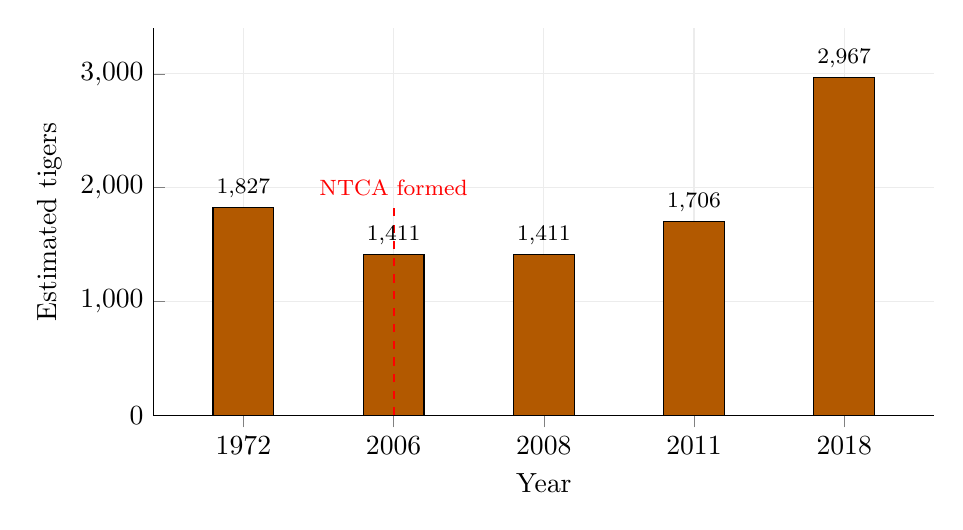
\begin{tikzpicture}
\begin{axis}[
  ybar, width=11.5cm, height=6.5cm,
  xlabel={Year}, ylabel={Estimated tigers},
  symbolic x coords={1972,2006,2008,2011,2018},
  xtick=data,
  ymin=0, ymax=3400,
  nodes near coords, nodes near coords style={font=\footnotesize},
  bar width=22pt,
  axis lines*=left,
  enlarge x limits=0.15,
  grid=major, grid style={gray!15}
]
\addplot[fill=orange!70!black] coordinates {
  (1972,1827) (2006,1411) (2008,1411) (2011,1706) (2018,2967)
};
\draw[dashed, red, thick] (axis cs:2006,0) -- (axis cs:2006,1850);
\node[red, font=\footnotesize] at (axis cs:2006,2000) {NTCA formed};
\end{axis}
\end{tikzpicture}

\vspace{1mm}
\footnotesize The 1972 pre-Project-Tiger baseline is shown for reference (Project Tiger launched 1973). Numbers fell to their lowest documented point around 2006 (the low point that triggered the Wild Life (Protection) Amendment Act, 2006 and creation of the NTCA), then recovered steadily through 2008, 2011, and 2018 once camera-trap-based, statistically corrected monitoring (Karanth \& Nichols methodology) was adopted alongside the institutional reforms.
\end{figbox}

A consequence flagged directly on the slides as ``the result'' of recovering tiger (and more broadly wildlife) populations pressing against shrinking, fragmented habitat: rising \textbf{human--animal conflict}, illustrated with both tiger and elephant examples (e.g.\ trials of Indian Railways interventions to reduce elephant deaths from train collisions, and the use of lemon/chilli-based deterrent plantings in Assam to keep elephants from raiding crops).

\subsubsection{Taking a global view}
The slides note that \textbf{roughly 70\% of the world's wild tigers are found in India} -- making India's conservation performance disproportionately important to the species' global survival prospects -- and situate this within the broader international legal framework of \textbf{CITES (the Convention on International Trade in Endangered Species of Wild Fauna and Flora), established in 1973}, a global treaty regulating trade in endangered plants and animals (directly relevant to controlling the illegal trade in tiger parts that drives poaching).

\begin{papbox}[title={Paper Summary: Karanth, K.U.\ \& Nichols, J.D.\ (2010), ``Non-invasive Survey Methods for Assessing Tiger Populations,'' in Tilson, R.\ \& Nyhus, P.J.\ (eds), \textit{Tigers of the World: The Science, Politics, and Conservation of Panthera tigris}, Elsevier}]
\textbf{Scope and motivation:} A methodological review chapter addressing a problem directly relevant to the Project Tiger numbers above: how do you actually \emph{count} a secretive, low-density, wide-ranging carnivore reliably enough to detect real population trends (rather than survey-method noise)? The authors are highly critical of India's traditional \textbf{pugmark census} method (identifying individual tigers from footprint/track impressions), used for decades in official government tiger counts, arguing it is fundamentally an uncorrected \emph{index} of abundance -- it assumes, without justification, that detectability of tigers (and of their tracks, under varying substrate and observer conditions) is constant across space, time, and observers, and its individual-identification claims from pugmark shape have never been rigorously validated. This critique is precisely why some of the headline Project Tiger figures above (e.g.\ the post-launch ``over 4,000'' figure) are explicitly flagged on the lecture slides as ``questioned.''

\textbf{The general statistical framework the authors advocate:} almost any wildlife count $C$ obtained from a survey is related to the true population size $N$ by $C = N \times p$, where $p$ is the (typically $<1$ and variable) probability of detecting an individual during the survey. Rearranging, $N = C/p$ -- so a valid abundance estimate \emph{requires} an explicit, empirically estimated detection probability $p$, not just a raw count or index, which is exactly what pugmark-based ``censuses'' fail to provide.

\textbf{Method 1 -- camera-trap capture--recapture (site-level abundance and density):} Tigers have individually distinctive stripe patterns, allowing camera-trap photographs to serve as ``captures'' in a formal \textbf{capture--recapture} framework, directly analogous to physically marking and recapturing animals but fully non-invasive. Paired camera stations are systematically placed across a grid spanning the study area (spacing chosen relative to tiger home-range size, so that no individual's home range can fall entirely between stations), and run over a short trapping session (on the order of a few weeks to ~2 months) chosen to be short enough that the population can reasonably be treated as \textbf{demographically and geographically closed} (no births/deaths/immigration/emigration during sampling). The resulting individual capture histories are analyzed with \textbf{closed-population capture--recapture models} (in the tradition of Otis et al.\ 1978's model set $M_0, M_t, M_b, M_h$), with the authors emphasizing that the \textbf{heterogeneity model $M_h$} (allowing capture probability to vary by individual -- e.g.\ dominant, wide-ranging males are typically easier to photograph than shy females with small home ranges) is usually the most biologically realistic choice for tigers, since assuming equal, constant capture probability across individuals ($M_0$) would bias abundance estimates. To convert the abundance estimate for the trapped area into a \textbf{density} estimate (individuals per unit area, the quantity actually needed to compare sites or extrapolate to unsurveyed habitat), the authors discuss the difficulty of defining the true ``effectively sampled area'' -- since some photographed tigers' home ranges only partly overlap the trapping grid -- typically handled by adding a buffer strip around the trapping grid based on estimates of tiger movement distances (e.g.\ mean maximum distance moved between capture locations).

\textbf{Method 2 -- occupancy modelling (landscape-level distribution):} For questions at larger, landscape-to-regional scales (where exhaustive camera-trapping everywhere is infeasible), the authors advocate \textbf{sign-based occupancy surveys}: repeated searches of many spatial sampling units (grid cells) for indirect tiger signs (tracks, scat, scrape marks), generating detection/non-detection histories per cell. These are analyzed with \textbf{occupancy models} (following MacKenzie et al.) that, analogously to the capture--recapture logic above, explicitly estimate and correct for an imperfect per-visit \textbf{detection probability}, yielding an estimate of the true proportion of the landscape occupied ($\psi$), rather than the naive (downward-biased) proportion of cells where a sign happened to be found.

\textbf{Conclusion / the paper's central message:} the authors argue strongly for \textbf{replacing ad hoc, uncorrected index-based methods (like the traditional pugmark census) with model-based estimators that explicitly account for imperfect detection}, at two complementary spatial scales -- camera-trap capture--recapture for rigorous abundance/density estimates at specific well-resourced sites, and sign-based occupancy modelling for broader landscape-level distribution and habitat-use monitoring where intensive camera-trapping is impractical. Adopting this statistically defensible, standardized toolkit (rather than methodologically inconsistent historical counts) is presented as essential infrastructure for actually being able to tell whether tiger conservation interventions -- like Project Tiger itself -- are working.
\end{papbox}

\begin{exambox}
A good synthesis question linking the two papboxes of this topic: \textbf{both the passenger pigeon and the tiger case studies show that ``the number looked fine until suddenly it wasn't''-type surprises trace back to methodological or mechanistic gaps in how the population was actually being tracked or was behaving at low density.} For the passenger pigeon, naive expectation (hunting stopped $\Rightarrow$ population should recover) failed because of an unmodelled Allee-type social/ecological mechanism (Bucher 1992). For the tiger, naive counts (pugmark-based indices) failed because they lacked a statistically valid detection-probability correction (Karanth \& Nichols 2010), which is precisely why some official Project Tiger figures are questioned and why the shift to camera-trap capture--recapture and occupancy modelling was such a significant methodological advance.
\end{exambox}

\subsection{Summary}
\begin{keybox}
This topic connected \textbf{conservation ethics} (Preservation vs.\ Resource Conservation vs.\ Land Ethic -- why we should conserve at all, and what ``success'' even means) to the \textbf{population-ecology science of vulnerability} (Rabinowitz's rarity classification; demographic, genetic, and environmental stochasticity; Minimum Viable Population) and then to \textbf{two detailed case studies} illustrating both sides of the coin. The \textbf{passenger pigeon} shows how a species that was, by simple numbers, about as ``un-rare'' as imaginable could nonetheless collapse to extinction once hunting pushed it below a threshold at which its own social/ecological biology (large-flock dependence for food-finding and predator-swamping) turned against it -- and how genuinely uncertain science can remain even for a thoroughly studied historical extinction (the unresolved role of genetics). \textbf{Project Tiger} shows the flip side: a large-scale, politically-backed conservation intervention that produced real early gains, suffered serious reversals when the ``four things'' (science, common sense, economics, politics) stopped converging, and was ultimately only properly evaluable once the \emph{survey science itself} was put on rigorous statistical footing (capture--recapture and occupancy modelling replacing index-based pugmark counts). The unifying lesson the course draws: effective conservation needs sound ethics/politics to motivate action, sound ecological theory to know what to protect against, and sound \emph{statistical} methodology to actually know whether the intervention is working -- Project Tiger's own history shows what happens when any one of these pieces is missing or comes under strain.
\end{keybox}

\end{document}
